% !TEX TS-program = LuaLaTeX
\documentclass[oneside]{book}

\usepackage[T1]{fontenc}
\usepackage{lmodern}
\usepackage{xcolor}
    \definecolor{gray} {HTML}{363636}
    \definecolor{red}  {HTML}{950009}
    \definecolor{green}{HTML}{0E610A}
    \definecolor{blue} {HTML}{020069}
\usepackage{fontspec}
    \setsansfont{Arial}
\usepackage{amsmath}
\usepackage{geometry}
    \geometry{scale={0.75,0.85}}
\usepackage{siunitx}
    \sisetup{locale=FR}
    \sisetup{math-micro=\text{µ},text-micro=µ} % fix
\usepackage{graphicx}
\usepackage{caption}
    \captionsetup{labelfont={bf,sf,color=gray}}
\usepackage{pdfpages}
\usepackage{caption}
\usepackage[titletoc]{appendix}
\usepackage{appendix}
\usepackage{chngcntr}
% Glossaire
\usepackage{glossaries}
\newglossaryentry{<mot à utiliser pour appeler le terme du glossaire>}
{%
	name={<terme>}, % le terme à référencer (l'entrée qui apparaitra dans le glossaire)
	description={<description>} % la description du terme (sans retour à la ligne)
}
\makeglossaries

\usepackage{mwe} % For dummy images
\usepackage{subcaption}

\usepackage{fancyhdr}
\pagestyle{fancy}
\fancyhead[R]{}
\fancyfoot[C]{}
\fancyfoot[C]{}

\usepackage{rotating}
\usepackage{tikz}
\usepackage{enumitem}

\makeatletter
\let\original@addcontentsline\addcontentsline
\newcommand{\dummy@addcontentsline}[3]{}
\newcommand{\DeactivateToc}{\let\addcontentsline\dummy@addcontentsline}
\newcommand{\ActivateToc}{\let\addcontentsline\original@addcontentsline}
\makeatother

\usepackage{listings}             % Include the listings-package

\usepackage{amsthm}
\newtheorem{definition}{Définition}[section]

% Keep lasts
\usepackage[french]{babel}
    \frenchsetup{SmallCapsFigTabCaptions=false}
\usepackage[expansion]{microtype}
\usepackage[luatex, backref]{hyperref}
    \hypersetup{unicode, colorlinks, breaklinks, urlcolor=red,
                bookmarksopen, bookmarksnumbered}

\renewcommand{\UrlFont}{\small}
\renewcommand{\arraystretch}{1.1}
\setlength{\parskip}{2mm}

% Chapters & sections
\usepackage[Lenny]{fncychap}



\begin{document}

%%%%%%%%%%%%%%%%%%%%%%%%%%%%%%%%%%%%%%%%%%%%%%%%%%%%%%%%%%%%%%
%                                                                           Page de couverture                     								 %
%%%%%%%%%%%%%%%%%%%%%%%%%%%%%%%%%%%%%%%%%%%%%%%%%%%%%%%%%%%%%%
\thispagestyle{empty}

\vspace{2cm}
\begin{center}
	\centerline{\textbf{Haute École Léonard De Vinci}}
	
\includegraphics[scale=0.15]{logos/logo-ecam.png}\\
	\centerline{\textbf{A.S.B.L.}}
	\vspace{3cm}

	\rule[0.5ex]{\linewidth}{2pt}\vspace*{-\baselineskip}\vspace*{3.2pt}
	\rule[0.5ex]{\linewidth}{1pt}\\[\baselineskip]
	{\Large \textit{Implémentation d'une contre-mesure face à une attaque par analyse de la consommation de puissance d'un circuit intégré de chiffrement AES}}\\
	\vspace{4mm}
	\rule[0.5ex]{\linewidth}{1pt}\vspace*{-\baselineskip}\vspace*{4pt}
	\rule[0.5ex]{\linewidth}{2pt}\\[\baselineskip]

\end{center}

\vspace{5cm}
      \begin{flushright} \large
        Travail de fin d'étude présenté par 

        Thomas ANIZET
        
        En vue de l'obtention du diplôme de
        
        Master en Sciences de l’Ingénieur Industriel orientation Electronique
      \end{flushright}
\vspace{9mm}

\vfill 
\centerline{\textbf{Année académique 2018-2019}}

% Laisser une page vierge
\newpage
\strut
\thispagestyle{empty}
\newpage
\fancyfoot[C]{\thepage}

%%%%%%%%%%%%%%%%%%%%%%%% Abstract %%%%%%%%%%%%%%%%%%%%
\pagenumbering{Roman}
\phantomsection
\addcontentsline{toc}{chapter}{Abstract} %Pour l'ajout dans la table des matières au même rang que chapitre
\pdfbookmark{bookmark}{hyperrefuid}
\null\vfil
\section*{\centering Abstract}

Imaginez que de simples analyses de paramètres physiques (température, consommation de puissance, rayonnement électromagnétique) permettent de révéler les secrets de votre carte d'identité ou de votre carte bancaire ?  
Ceci est aujourd'hui possible depuis la découverte fin des années 1990 d'un nouveau type d'attaque ciblant les algorithmes de chiffrement : les attaques par canaux auxiliaires. À ce jour, il existe une multitude d’algorithmes de chiffrement. L’algorithme \textit{AES} (\textit{Advanced Ecryption Standard}) est sans nul doute le plus réputé et le plus répandu, de nos jours, dans la majeure partie des systèmes embarqués comportant des applications en sécurité. L'attaque par \textit{l'analyse de la consommation de puissance} est un exemple parmi d'autres d'attaques par canaux auxiliaires d'un système implémentant l'algorithme AES. Cette attaque analyse la consommation de puissance du device cryptographique lorsque celui-ci chiffre les données. En effet, la puissance consommée par le circuit intégré reflète directement ses activités internes (instructions exécutées et données manipulées). Depuis ces découvertes, la sécurité matérielle a pris une tournure particulière. C’est désormais sur un nouvel axe de recherche, s’écartant des sentiers traditionnels, que se porte la problématique de protection des données sensibles.

Étant un acteur majeur dans le domaine de la Défense, Thales collabore étroitement avec de nombreux gouvernements. La cybersécurité est au centre des préoccupations actuelles. Le besoin en implémentations sécurisées se fait de plus en plus ressentir. Il est nécessaire de se prémunir contre les attaques classiques mais également contre les attaques de plus bas niveau exploitant des caractéristiques physiques. L'attaque ciblée dans ce \textit{Travail de Fin d'Étude} (TFE) concerne l'analyse de la consommation de puissance. Mon objectif est le suivant : dans un premier temps, réaliser une série de démonstrateurs permettant de mettre en évidence l'impact des failles non traitées. Dans un second temps, développer une contre-mesure et justifier son gain en sécurité.


\newpage
\strut
\thispagestyle{empty}
\newpage


%%%%%%%%%%%%%%%%%%%%%%%% Remerciements %%%%%%%%%%

\phantomsection
\chapter*{Remerciements}
\addcontentsline{toc}{chapter}{Remerciements}

Encore à compléter...

Je tiens à remercier toutes les personnes qui ont permis à ce travail de voir le jour, mais qui m’ont également soutenu tout au long de ces 5 années d’étude à l’ECAM.

Je remercie \textit{Thales Belgium Communications \& Security} de m’avoir permis de réaliser mon stage et mon TFE.

Je remercie tout particulièrement Monsieur Liran Lerman, mon promoteur, de m’avoir proposé ce projet très intéressant et qui fut très enrichissant. Je le remercie pour son support précieux, sa disponibilité mais également pour ses conseils et ses encouragements quotidiens.

Je remercie Monsieur François Durvaux, pour ses précieux conseils et ses connaissances avancées dans le domaine des attaques par canaux auxiliaires. Il m'a permis d'avancer rapidement dans mon travail.

Je remercie Monsieur Arnaud, pour son temps précieux consacré à m'apprendre de nouveaux concepts sur la programmation orientée hardware. 

Je remercie également mademoiselle Clémence Flémal, ma tutrice, qui m’a accompagné dans la réalisation de ce travail et qui m’a consacré son temps et son attention durant la période de stage et de TFE.

\newpage

%%%%%%%%%%%%%%%%%%%%%%%% Cahier des charges %%%%%%%%%%

\phantomsection
\addcontentsline{toc}{chapter}{Cahier des charges} %Pour l'ajout dans la table des matières au même rang que chapitre

\begin{center}
	
\includegraphics[scale=0.1]{logos/logo-ecam.png}\\
\end{center}
\hspace{-0.5 cm}\fbox{
\begin{minipage}{\textwidth}
\centering
\textbf{\Large{Cahier des charges relatif au travail de fin d'études de}} \\
\vspace{0.5cm}\Large{Thomas ANIZET, inscrit en 2\up{ème} Master, orientation électronique}
\end{minipage}
}

\vspace{1cm}
\begin{itemize}[label=$\bullet$]
\item \underline{Année académique} : 2018-2019 \\ \\
\item \underline{Titre provisoire} : Contre-mesure pour les attaques par canaux cachés \\ \\
\item \underline{Objectifs à atteindre} : Étant un acteur majeur dans le domaine de la Défense, Thales collabore étroitement avec de nombreux gouvernements. La cybersécurité est au centre des préoccupations actuelles. Le besoin en implémentations sécurisées se fait donc de plus en plus ressentir. L’objectif est de se prémunir contre des attaques classiques et des attaques plus bas niveau exploitant des caractéristiques physiques. Afin de se familiariser avec ce domaine, l’étudiant devra réaliser une recherche bibliographique de règles de bonnes pratiques pour de la programmation sécurisée hardware. Après en avoir étudié les tenants et aboutissants, l’étudiant réalisera (\textit{i}) une série de démonstrateurs permettant de mettre en évidence l’impact des failles non traitées et (\textit{ii}) le gain en sécurité dû aux contre-mesures. \\ \\
\item \underline{Principales étapes} : \begin{itemize}
\item  Recherches bibliographiques de règles de bonnes pratiques.
\item Implémentation de l’algorithme AES sur FPGA.
\item Réalisation d’une attaque CPA (Correlation Power Analysis).
\item Étude et choix de métrique(s) pour l’analyse de contre-mesures.
\item Développement d’une contre-mesure.
\item Analyse et conclusion sur la contre-mesure développée. \\ \\ \\ \\ \\ \\ \\ \\
\end{itemize}

\hfill Fait en trois exemplaires à Tubize, le 22 Novembre 2018.
\end{itemize}


\newpage

%%%%%%%%%%%%%%%%%%%%%%%%%%%%%%%%%%%%%%%%%%%%%%%%%%%%%%%%%%%%%%
%                                                                           Table des matières                     								 %
%%%%%%%%%%%%%%%%%%%%%%%%%%%%%%%%%%%%%%%%%%%%%%%%%%%%%%%%%%%%%%

\tableofcontents
\newpage

%%%%%%%%%%%%%%%%%%%%%%%%%%%%%%%%%%%%%%%%%%%%%%%%%%%%%%%%%%%%%%
%                                                                           Liste des figures                      								 %
%%%%%%%%%%%%%%%%%%%%%%%%%%%%%%%%%%%%%%%%%%%%%%%%%%%%%%%%%%%%%%

\listoffigures
\newpage

%%%%%%%%%%%%%%%%%%%%%%%%%%%%%%%%%%%%%%%%%%%%%%%%%%%%%%%%%%%%%%
%                                                                           Liste des tableaux                       								 %
%%%%%%%%%%%%%%%%%%%%%%%%%%%%%%%%%%%%%%%%%%%%%%%%%%%%%%%%%%%%%%

\listoftables
\newpage

%%%%%%%%%%%%%%%%%%%%%%%%%%%%%%%%%%%%%%%%%%%%%%%%%%%%%%%%%%%%%%
%                                                                        Liste des acronymes                       								 %
%%%%%%%%%%%%%%%%%%%%%%%%%%%%%%%%%%%%%%%%%%%%%%%%%%%%%%%%%%%%%%

\phantomsection
\chapter*{Liste des acronymes}
\addcontentsline{toc}{chapter}{Liste des acronymes}

\hspace{-0.5 cm}Encore à compléter ... \\ \\
\hspace{-0.5cm}\textbf{AES} \hfill Advanced Encryption Standard \\ \\
\textbf{CMOS} \hfill Complementary Metal Oxyde Semiconductor \\ \\
\textbf{CPA} \hfill Correlation Power Analysis \\ \\
\textbf{DPA} \hfill Differential Power Analysis \\ \\
\textbf{FPGA} \hfill Field Programmable Gate Array \\ \\
\textbf{NIST} \hfill National Institute of Standard and Technology \\ \\
\textbf{RSA} \hfill Rivest Shamir Adleman \\ \\
\textbf{SPA} \hfill Simple Power Analysis \\ \\
\textbf{SNR} \hfill Signal-to-Noise Ratio \\ \\
\textbf{VHDL} \hfill VHSIC Hardware Description Language \\ \\
\textbf{XOR} \hfill Exclusive OR \\ \\

% Laisser une page vierge
\newpage
\strut
\thispagestyle{empty}
\newpage
\pagenumbering{arabic}

%%%%%%%%%%%%%%%%%%%%%%%%%%%%%%%%%%%%%%%%%%%%%%%%%%%%%%%%%%%%%%
%                                                                           Introduction générale                     								 %
%%%%%%%%%%%%%%%%%%%%%%%%%%%%%%%%%%%%%%%%%%%%%%%%%%%%%%%%%%%%%%

%%%%%%%%%%%%% Chapitre 1 %%%%%%%%%%%%%

\chapter{Introduction}

\section{Présentation du problème}

Le monde dans lequel nous vivons aujourd’hui est un monde où tout doit être connecté. Notre smartphone, notre montre, notre TV, notre frigo, notre tondeuse, … Tout système d’électronique embarquée est potentiellement connectable ! Les transferts d’informations sont par conséquent de plus en plus gourmands. Les technologies ne cessent d’évoluer. Le meilleur exemple est le développement de l'IoT (\textit{Internet of Things}) ou encore le développement du réseau 5G, prévu entre-autres pour augmenter les débits de données. Cependant, nous sommes en droit de nous poser plusieurs questions : toutes ces données qui voyagent de système en système sont-elles protégées ? Toutes ces données qui transitent entre les différents appareils connectés de ma maison peuvent-ils être captées par des pirates informatiques ? La réponse à ces deux questions reste bien souvent assez vague. Tentons de cerner le sujet.

Depuis toujours, l’homme cherche à dissimuler des informations à ses tiers mais depuis toujours, l’homme cherche également à accéder à des informations auxquelles il n’a pas droit. Cette lutte symbolise le combat entre la \textbf{cryptographie} et la \textbf{cryptanalyse}. Rappelons brièvement que la cryptographie a pour objectif de crypter de l’information, c’est-à-dire qu’elle vise à élaborer des procédés assurant la confidentialité de données sensibles. La cryptanalyse quant à elle vise à décrypter des informations sensibles auxquelles elle n'a normalement pas accès. Ainsi, lorsqu'il s'agit de manipuler des informations secrètes, la question d'intégrité et de confidentialité des informations manipulées se pose inévitablement. C'est pour cette raison que des \textbf{algorithmes de chiffrement} sont développés et par la suite, la cryptanalyse tente d'y déceler des failles. À ce jour, il existe une multitude d'algorithmes de chiffrement, chacun possédant ses avantages et ses inconvénients. Celui étudié dans ce travail est \textbf{l'algorithme \textit{AES}} (\textit{Advanced Ecryption Standard}).

Initialement, la cryptanalyse se basait essentiellement sur la compréhension des procédés mathématiques utilisés dans les algorithmes en vue d'y déceler des failles. Devant ces attaques, les ingénieurs renforcèrent la complexité des algorithmes. Par ailleurs, fin du millénaire précédent, le \textit{NIST} (\textit{National Institute of Standards and Technology}) a encouragé le développement d’un nouveau standard d’algorithme de chiffrement difficilement envisageable à casser : l’algorithme \textit{AES}. Sa robustesse aux attaques classiques lui permet d'être considéré aujourd’hui comme l'algorithme le plus connu au monde et implémenté dans la majeure partie des systèmes embarqués comportant des applications en sécurité. Cependant, fin des années 1990, de nouvelles recherches dans le domaine de la cryptanalyse ont été réalisées. Ces recherches ont abouti sur un nouveau type d'attaque : les \textbf{attaques par canaux auxiliaires}. Une attaque par canal auxiliaire désigne une attaque informatique qui, sans remettre en cause la robustesse théorique des méthodes et procédures de sécurité, recherche et exploite des failles dans leur implémentation logicielle ou matérielle. 

\newpage
Il existe différents types d'attaques par canaux auxiliaires cependant ce travail se concentre sur un type d'attaque en particulier : les \textbf{attaques par analyse de la consommation de puissance}. Comme son nom l'indique, cette attaque analyse la consommation de puissance d'un \textbf{\textit{système cryptographique}} en cours de chiffrement. En effet, la puissance consommée par le circuit intégré reflète directement ses activités internes (instructions exécutées et données manipulées). Cette puissance consommée peut être capturée à l'aide d'un instrument de mesure tel que l'oscilloscope. Les mesures prélevées à l'oscilloscope portent le nom de \textit{traces de puissance}. Lorsque la clé d'un algorithme de chiffrement est révélée, le contenu censé rester confidentiel devient accessible à quiconque le souhaite. Ainsi, comme nous le verrons au chapitre X, dès que des traces de puissance sont acquises, il est possible pour un attaquant, via divers calculs, de retrouver la clé utilisée pour le chiffrement des données. Attirons l'attention sur le fait que l'attaque exploite les faiblesses du système cryptographique, c'est-à-dire du système implémentant l'algorithme de chiffrement (l'AES en l'occurence). En aucun cas, l'attaque exploite les failles des principes mathématiques mis en place.

\begin{figure}[h]
    \hspace{-1.55cm}
    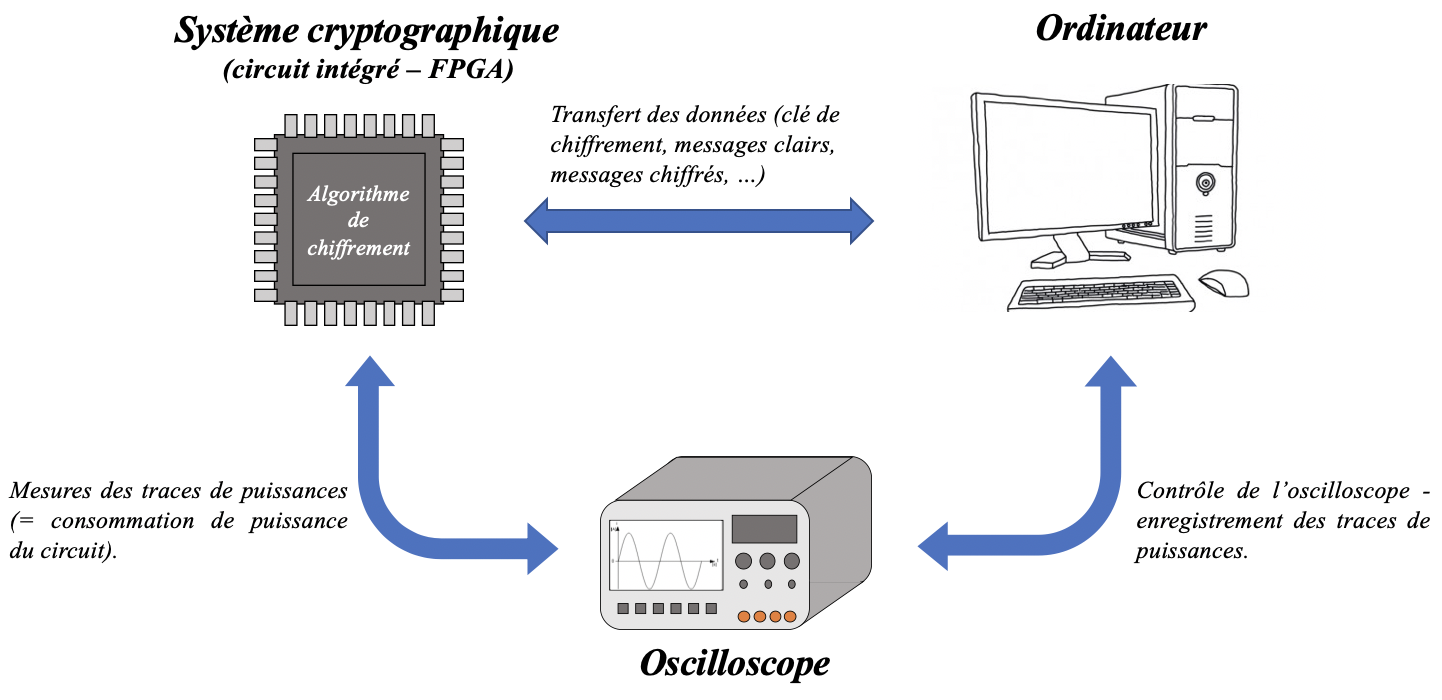
\includegraphics[scale=0.72]{image/intro.png}
    \caption{Matériel nécessaire pour réaliser une attaque par analyse de la consommation de puissance.}
    \label{fig:intro}
\end{figure}

Dès que ces attaques se sont manifestées, une série de contre-mesures a été développée. Pour obtenir une contre-mesure efficace contre ces attaques par analyse de la consommation de puissance, il est nécessaire de bien appréhender le fonctionnement de l'attaque. Ainsi, retenons que lors de l’exécution d’un algorithme de chiffrement, différentes opérations sont exécutées conduisant à différentes \textbf{valeurs intermédiaires calculées}. Si aucune protection n’est mise en place, la consommation de puissance du device cryptographique dépend des données intermédiaires manipulées par ce dernier (par l’algorithme précisément). Par conséquent, l’attaquant peut potentiellement retrouver la clé secrète en analysant la consommation de puissance du système. Dès lors, l'objectif général d'une contre-mesure est de rendre la consommation de puissance du device cryptographique indépendante des valeurs intermédiaires calculées par l'algorithme de chiffrement. 

Deux grands types de contre-mesures sont à distinguer : les contre-mesures de type \textbf{\textit{Masking}} et les contre-mesures de type \textbf{\textit{Hiding}}. Brièvement, le principe d'une contre-mesure de type \textit{Masking} est de modifier les caractéristiques de l'algorithme de chiffrement alors que le principe d'une contre-mesure de type \textit{Hiding} est de modifier les caractéristiques physiques du système cryptographique. La contre-mesure développée dans ce travail est une contre-mesure apparue assez récemment : la contre-mesure de type \textit{Faking}. Le principe de fonctionnement de cette contre-mesure se rapproche de celui de contre-mesure de type \textit{Masking}. Cependant, comme nous le verrons au chapitre X, il existe quelques subtilités. Le tableau \ref{fig:intro2} résume les constats qui peuvent être tirés selon qu'une contre-mesure soit implémentée ou non. Ces contre-mesures seront détaillées plus en profondeur au chapitre y faisant référence (chapitre X).

\begin{table}
	\centering
	\begin{tabular}{|l|m{9cm}|l|m{3cm}|}
    		\hline
   		 Avec/Sans contre-mesure & Conséquences \\ \hline
    		Sans contre-mesure & La consommation de puissance dépend directement des valeurs intermédiaires calculées par l’algorithme de chiffrement. \\ \hline
		Avec contre-mesure type Hiding & Modification des caractéristiques de consommation : La consommation de puissance du device cryptographique est identique (ou aléatoire) pour chaque instruction exécutée et chaque donnée manipulée. \\ \hline
    		Avec contre-mesure type Masking & Modification de l’algorithme : Les valeurs intermédiaires calculées par l’algorithme de chiffrement sont masquées par des valeurs aléatoires. La consommation de puissance est alors modifiée (les traces capturées à l’oscilloscope sont insensées). \\ \hline
		Avec contre-mesure type Faking & Modification de l’algorithme : La consommation de puissance du device cryptographique permet de trouver une valeur de clé secrète. Cependant, la clé obtenue est volontairement faussée en appliquant un masque sur la vraie clé. \\ \hline
 	\end{tabular}
 	\caption{Conséquences de l'implémentation d'une contre-mesure.}
 	\label{fig:intro2}
\end{table}

\newpage
Enfin, pour juger de \textbf{l'efficacité de la contre-mesure implémentée}, différentes analyses peuvent être réalisées. Ainsi, des métriques telles que le \textit{SNR} (\textit{Signal-Noise to Ratio}) peuvent être utilisées afin de savoir si les traces capturées à l'oscilloscope laissent fuiter de l'information ou non. Outre les métriques, une analyse des performances du système sera également établie. Les principales performances étudiées sont : le temps d'exécution de l'algorithme, la consommation de puissance du device cryptographique, la place mémoire de l'implémentation protégée de l'algorithme sur le device crytpographique, ...

\section{Structure du travail}

\hspace{-0.5cm}Ce travail est scindé en deux parties : 
\begin{enumerate}
\item La première partie aborde tous les concepts théoriques nécessaires afin de comprendre le fondement des attaques par canaux auxiliaires. Un premier chapitre expose les concepts et définitions de la cryptologie et définit en particulier le fonctionnement de l'algorithme AES. Le second chapitre est consacré à la consommation de puissance des circuits en technologie CMOS. Cette analyse de la consommation de puissance pour ce type de circuit en particulier permet de comprendre le principe de fonctionnement des attaques par analyse de la consommation de puissance. Le troisième chapitre définit le sujet principal de ce travail, à savoir les attaques par canaux auxiliaires. Enfin, le dernier chapitre étudie les différentes contre-mesures existantes afin d'assurer une meilleure protection des données sensibles. 
\item La seconde partie aborde les notions et compétences acquises durant la période de TFE. Un premier chapitre définit la configuration du matériel nécessaire pour implémenter l'attaque par analyse de la consommation de puissance. Un descriptif succinct des langages et matériels utilisés est ainsi détaillé. Le second chapitre reprend les résultats obtenus et leurs conclusions pour la mise en application d'une attaque CPA (\textit{Correlation Power Analysis}). Le troisième chapitre détaille l'implémentation de la contre-mesure de type \textit{faking}. Le quatrième chapitre discute de l'efficacité de la contre-mesure implémentée. Enfin, un cinquième chapitre est consacré à la conclusion de ce rapport.
\end{enumerate}


\newpage

%%%%%%%%%%%%%%%%%%%%%%%%%%%%%%%%%%%%%%%%%%%%%%%%%%%%%%%%%%%%%%
%                                                                            Partie 1 - Théorie                     								 %
%%%%%%%%%%%%%%%%%%%%%%%%%%%%%%%%%%%%%%%%%%%%%%%%%%%%%%%%%%%%%%

\part{Contexte théorique}

%%%%%%%%%%%%% Chapitre 2 %%%%%%%%%%%%%

\chapter{Cryptologie}
\label{chap:crypto}

Ce chapitre introduit au lecteur les fondamentaux en matière de cryptologie. Les différents concepts et définitions abordés ont pour but d'apporter au lecteur les connaissances nécessaires et suffisantes pour la bonne compréhension des chapitres suivants. Ce chapitre est scindé en deux parties. Dans un premier temps, il abordera les définitions importantes en matière de cryptologie et plus spécifiquement en matière de cryptographie. La cryptographie symétrique sera ainsi distinguée de la cryptographie asymétrique. Dans un second temps, ce chapitre détaillera le principe de fonctionnement général d'un algorithme de chiffrement. Une attention particulière sera finalement consacrée à la compréhension de l'algorithme AES.

\section{Concepts et définitions}
\label{sec:Concepts}

Il y a plus de 2000 ans naissait le concept de \textbf{cryptologie} avec la montée au pouvoir de Jules César. Général romain très puissant, César marqua le monde et l'histoire universelle au travers de ses nombreuses conquêtes. Tant adulé par son peuple, César s'était néanmoins fait plus d'un ennemi durant ses conquêtes. Le 15 mars 44 avant J-C, il fut tragiquement assassiné par une conspiration de sénateurs romains dont son fils, Marcus Junius Brutus. Jules César avait pris pour habitude de se méfier de ses ennemis. Arrivé à un stade de méfiance extrême, il n'avait plus confiance en ses propres messagers. C'est pour cette raison qu'il envoyait des messages chiffrés dans lesquels il décalait chaque lettre d'un mot de 3 lettres dans l'alphabet. Seul le destinataire, au courant de la règle de chiffrement, pouvait alors déchiffrer les messages. Ce fut le premier procédé de chiffrement de l'histoire, appelé \textit{Chiffre de César} (voir annexe \ref{ann:CESAR}). \\
C'est ainsi que tout commença...

Étymologiquement, le mot \textit{"cryptologie"} vient du grec et signifie littéralement la \textit{science du secret} (\textit{kryptos}  pour caché et \textit{logos} pour science). La cryptologie regroupe deux champs d'études diamétralement opposés : la cryptographie et la cryptanalyse.

\theoremstyle{definition}
\begin{definition}{\textbf{Cryptographie : }}
La cryptographie est la science qui utilise les mathématiques en vue de chiffrer et déchiffrer de l'information secrète.
\end{definition}

\begin{definition}{\textbf{Cryptanalyse : }}
La cryptanalyse est la science qui analyse les procédés mathématiques mis en place par la cryptographie en vue de retrouver de l'information secrète. 
\end{definition}

\hspace{-0.5cm}Six termes couramment employés en cryptologie doivent également être définis : 
\begin{description}
\item[Texte clair :] Il s'agit de données brutes, considérées comme confidentielles, compréhensibles sans intervention spécifique.
\item[Texte chiffré :] Il s'agit de données modifiées, considérées comme confidentielles et devant le rester. Ces données sont incompréhensibles, inintelligibles pour quiconque qui tenterait de les comprendre. 
\item[Chiffrement (cryptage) :] Procédé utilisé pour dissimuler le texte clair. Le chiffrement transforme donc le texte clair en texte chiffré.
\item[Déchiffrement (décryptage) :] Procédé inverse au chiffrement. Le déchiffrement transforme donc le texte chiffré en texte clair, c'est-à-dire en texte d'origine.
\item[Algorithme de chiffrement :] Fonctions mathématiques utilisées lors du processus de chiffrement. Les fonctions mathématiques inverses sont également définies pour le processus de déchiffrement.
\item[Clé de chiffrement :] Paramètre associé à l'algorithme de chiffrement pour le cryptage des textes clairs ou pour le décryptage des textes chiffrés. \\
\end{description}

\hspace{-0.5cm}La figure \ref{fig:fondamentaux_crypto} illustre cinq des six termes fondamentaux énoncés. Le sixième, l'algorithme de chiffrement, pourrait être confondu avec les étapes de \textit{chiffrement} et \textit{déchiffrement}. Cependant, une explication plus détaillée est donnée à la section \ref{sec:algo}.

\begin{figure}[htbp]
    \centering
    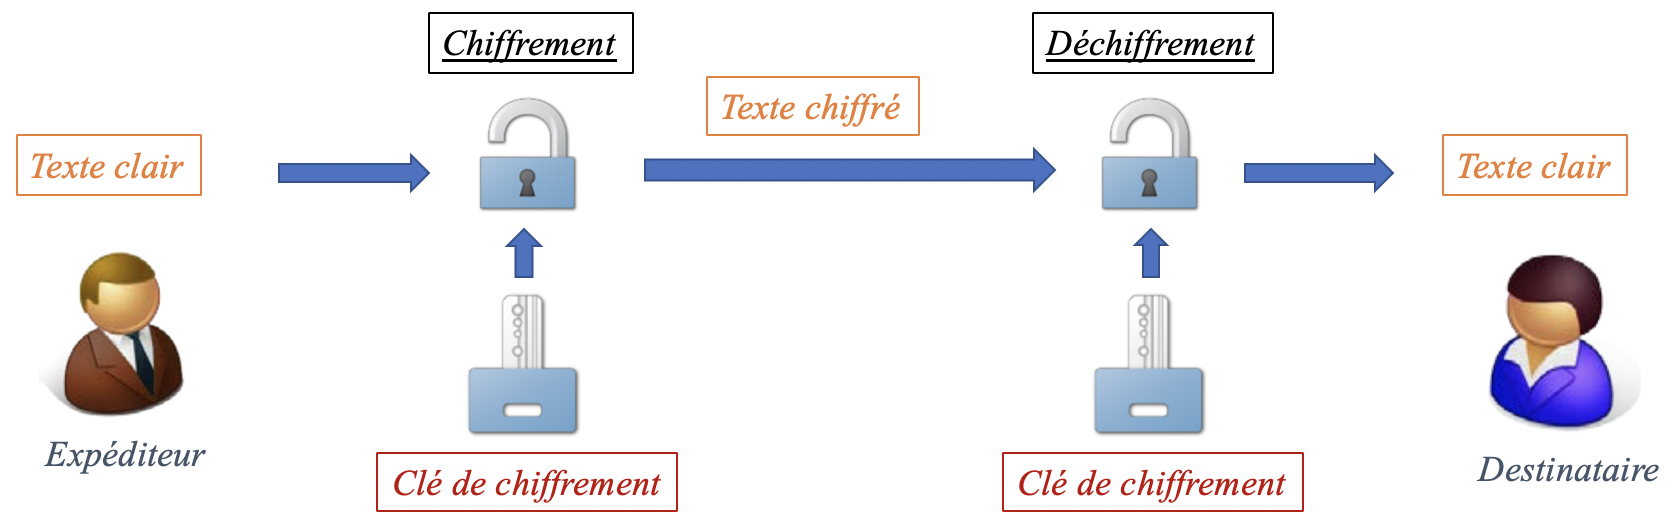
\includegraphics[width=0.85\textwidth]{image/fondamentaux_crypto}
    \caption{Concepts de chiffrement et de déchiffrement.}
    \label{fig:fondamentaux_crypto}
\end{figure}


\hspace{-0.5cm}Revenons sur la notion de cryptographie. La cryptographie doit remplir trois conditions majeures qui sont :
\begin{itemize}
\item \textbf{Confidentialité} : La confidentialité spécifie que seules les personnes autorisées à accéder à une certaine information ont la possibilité de l'atteindre.
\item \textbf{Intégrité} : L'intégrité spécifie que l'information, lors de son traitement ou de sa transmission, ne subit aucun modification volontaire ou accidentelle. Autrement dit, il s'agit d'une garantie que l'information conserve son état d'origine.
\item \textbf{Disponibilité} : La disponibilité spécifie que l'information est en tout temps disponible pour une personne autorisée à y accéder et en demandant l'accès. \\
\end{itemize}

Ainsi, la cryptographie a pour objectif de chiffrer des informations tout en assurant la confidentialité, l'intégrité et la disponibilité de ces informations. La cryptographie se divise en deux catégories distinctes : la cryptographie symétrique et la cryptographie asymétrique. 

\subsection{Chiffrement symétrique}
\label{subsec:Chiffrement_symétrique}

\theoremstyle{definition}
\begin{definition}{\textbf{Chiffrement symétrique :}}
Le chiffrement est dit symétrique lorsque la clé utilisée pour le chiffrement et le déchiffrement des données est la même. La clé est alors appelée \textit{clé secrète}. 
\end{definition}

\hspace{-0.5cm}Par convention, ce type de chiffrement permet à la fois de chiffrer et de déchiffrer des messages à partir d'une seule et unique clé : la clé secrète. Le désavantage de ce type de chiffrement est que si une personne parvient à subtiliser la clé, elle sera en mesure de déchiffrer tout message qu'elle intercepte. 

\hspace{-0.5cm}\textit{Exemple} : L'algorithme AES. Une explication plus détaillée de cet algorithme est reprise à la section \ref{subsec:AES}.


\hspace{-0.5cm}La figure \ref{fig:symétrique} (page suivante) présente le principe de fonctionnement du chiffrement symétrique. Comme le présente la figure, si un attaquant intercepte un message, ce dernier sera chiffré. Il doit donc être en possession de la clé secrète s'il souhaite comprendre le message envoyé par l'expéditeur.

\begin{figure}[htbp]
    \centering
    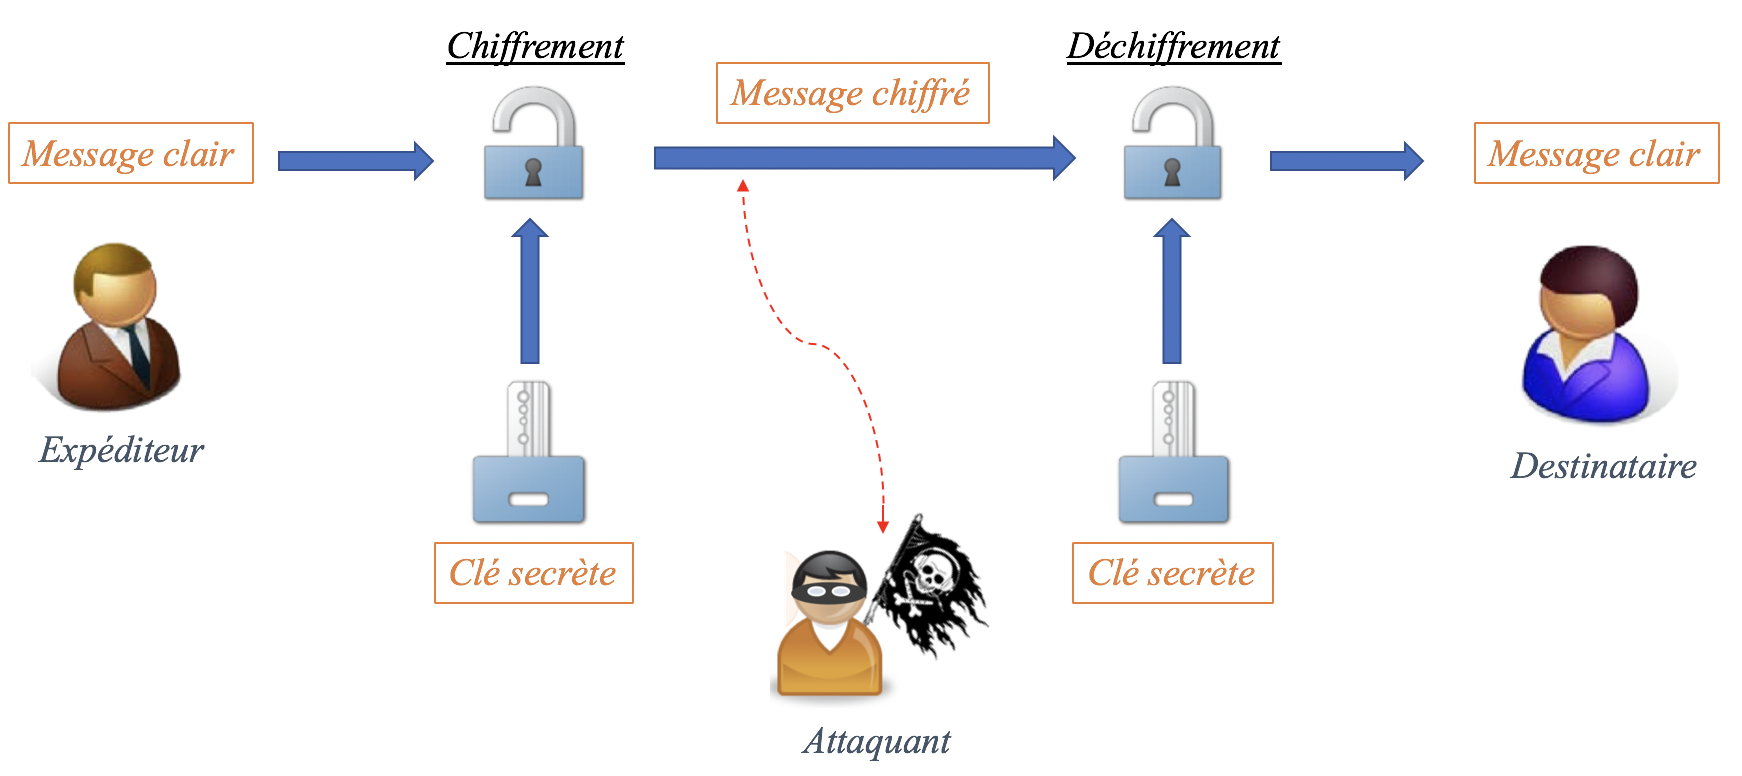
\includegraphics[width=0.75\textwidth]{image/symetrique}
    \caption{Chiffrement symétrique : Une seule clé est utilisée pour chiffrer et déchiffrer les messages.}
    \label{fig:symétrique}
\end{figure}


\newpage
\subsection{Chiffrement asymétrique}
\label{subsec:Chiffrement_asymétrique}

\theoremstyle{definition}
\begin{definition}{\textbf{Chiffrement asymétrique :}}
Le chiffrement est dit asymétrique lorsqu'il existe une clé publique utilisée pour le chiffrement des textes clairs et une clé privée utilisée pour le déchiffrement des textes chiffrés. 
\end{definition}

\hspace{-0.5cm}Par convention, la clé publique est la clé de chiffrement du message clair, elle peut être communiquée sans aucune restriction tandis que la clé privée est la clé de déchiffrement du message chiffré, elle ne doit être communiquée sous aucun prétexte. Le fonctionnement est le suivant : Avec une clé publique, l'expéditeur envoie un message chiffré selon un algorithme de chiffrement préalablement défini. Ce message, une fois transmis, ne pourra être déchiffré que par le destinataire, détenteur de la clé privée. \\
\textit{Exemple} : L'algorithme RSA (\textit{Rivest Shamir Adleman}).

\hspace{-0.5cm}La figure \ref{fig:asymétrique} ci-dessous présente le principe de fonctionnement du chiffrement asymétrique.

\begin{figure}[htbp]
    \centering
    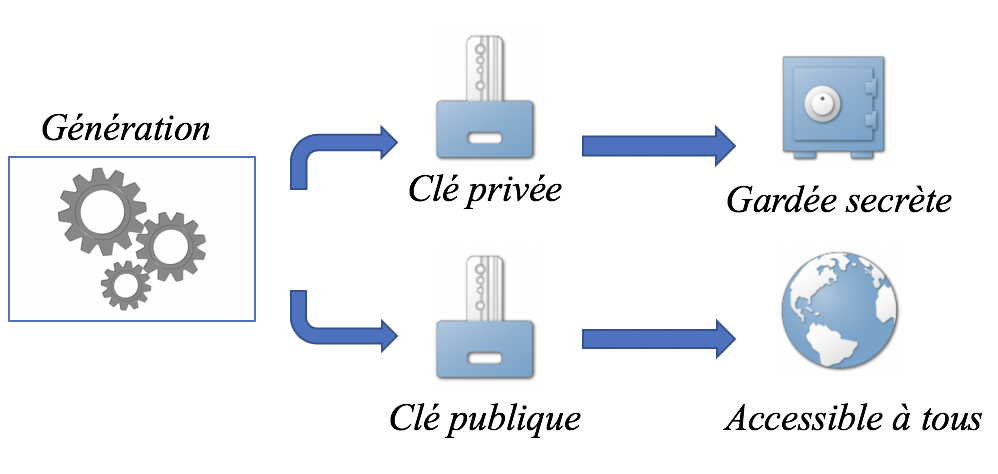
\includegraphics[width=0.5\textwidth]{image/cle_asymetrique}
    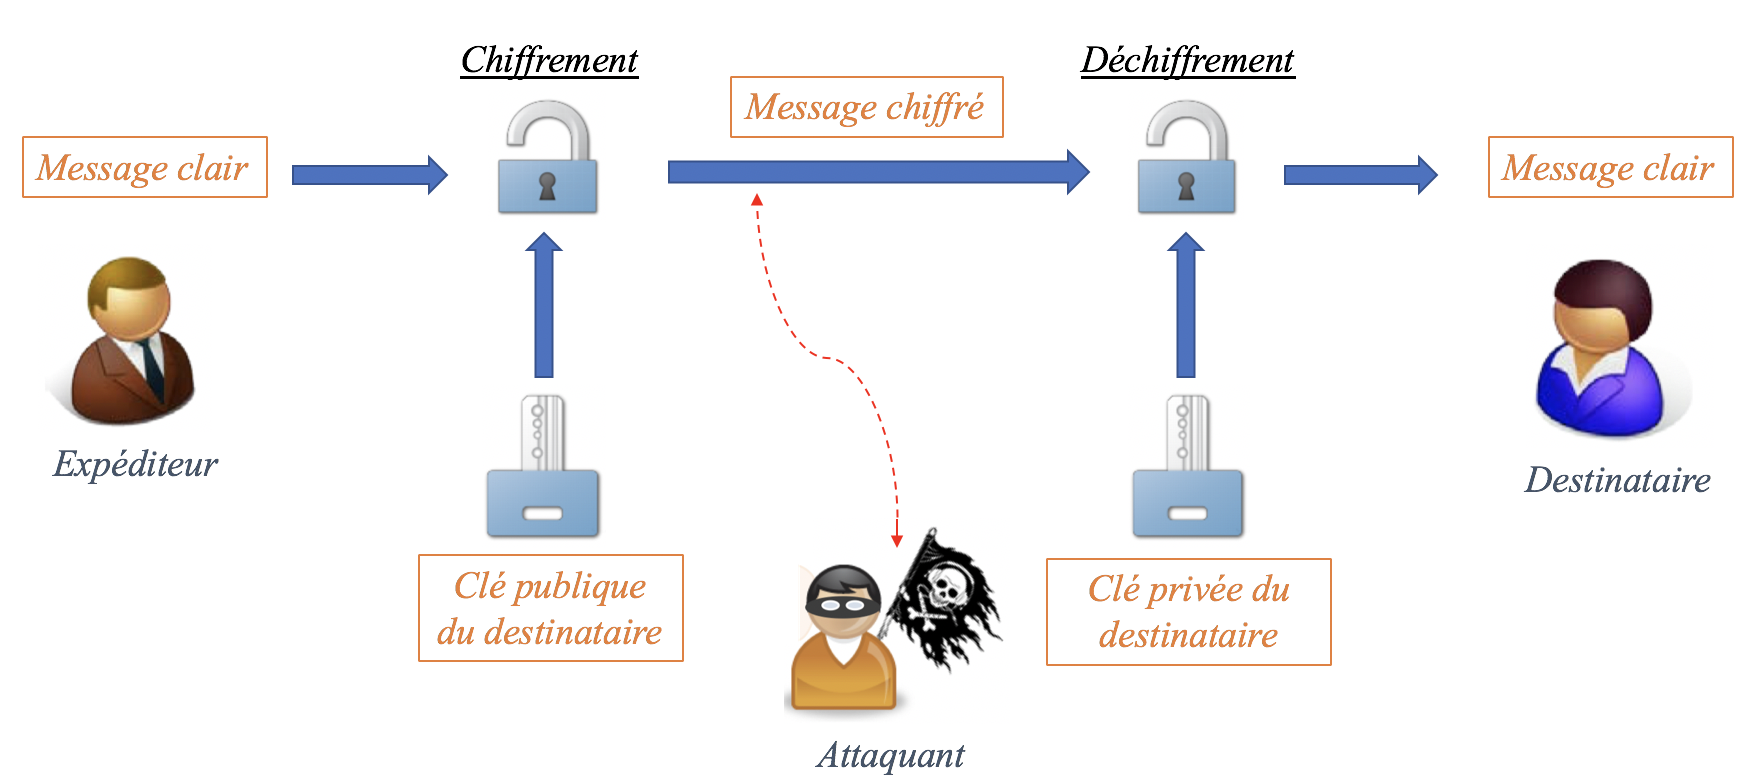
\includegraphics[width=0.75\textwidth]{image/asymetrique}
    \caption{Chiffrement asymétrique : Un clé publique est utilisée pour chiffrer le message et une clé privée est utilisée pour le déchiffrer.}
    \label{fig:asymétrique}
\end{figure}

\newpage
\section{Algorithme de chiffrement}
\label{sec:algo}

\subsection{Principe}
\label{sec:Introduction}

\theoremstyle{definition}
\begin{definition}{\textbf{Algorithme de chiffrement :}}
Un algorithme de chiffrement est un ensemble de fonctions mathématiques utilisé lors du processus de chiffrement et de déchiffrement de données sensibles. Une clé publique ou privée est associée à l'algorithme de chiffrement selon qu'il s'agisse d'un chiffrement symétrique ou asymétrique.
\end{definition}

\hspace{-0.5cm}Les systèmes de sécurité modernes utilisent des algorithmes de chiffrement pour assurer la confidentialité et l'intégrité de données sensibles. Ces algorithmes prennent typiquement : 
\begin{itemize}
\item  2 paramètres en entrée : un \textbf{\textit{message clair}} et une \textbf{\textit{clé de chiffrement}}.
\item 1 paramètre en sortie : le \textbf{\textit{message chiffré}}. \\
\end{itemize}
Comme décrit précédemment, le procédé transformant les données claires en entrée en données chiffrées en sortie est appelé \textit{chiffrement}. Ce procédé est réalisé grâce à un algorithme de chiffrement manipulant une clé de chiffrement, un message clair et diverses opérations mathématiques. Avec des clés différentes, le résultat du cryptage variera également. La figure \ref{fig:chiffrement} ci-dessous présente le principe de fonctionnement d'un algorithme de chiffrement.

\begin{figure}[htbp]
    \centering
    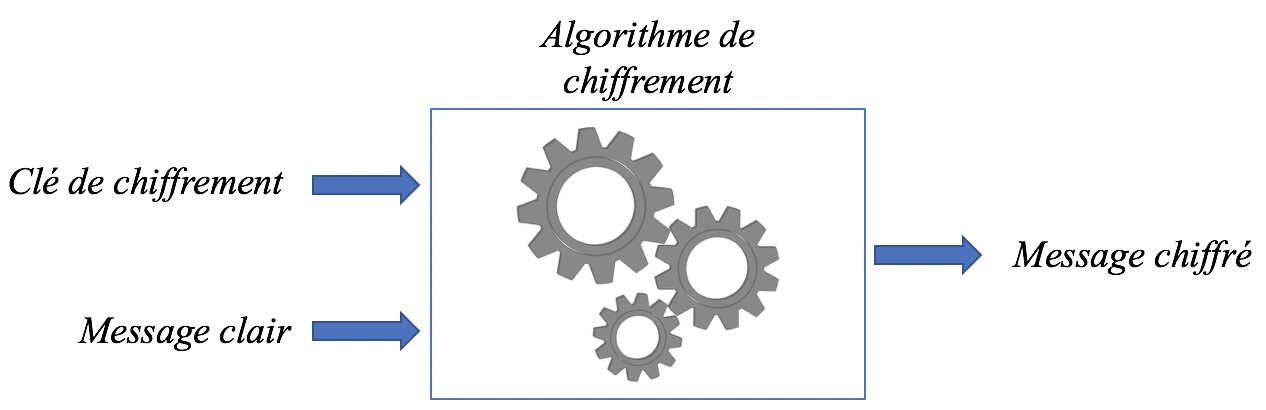
\includegraphics[width=0.8\textwidth]{image/chiffrement}
    \caption{Concept d'un algorithme de chiffrement.}
    \label{fig:chiffrement}
\end{figure}

Il est important de préciser que tous les détails décrivant le fonctionnement d'un algorithme cryptographique sont disponibles publiquement, seule la clé de chiffrement doit rester secrète. En effet, un principe fondamental de la cryptographie est le principe de Kerckhoffs. Ce principe stipule que la sécurité de tout algorithme de chiffrement ne doit pas reposer sur la connaissance du fonctionnement de ce dernier. Autrement dit, la sécurité offerte par un algorithme de chiffrement ne doit pas dépendre du secret de son implémentation mais doit uniquement reposer sur la protection de la clé, ou plus généralement d'un secret. Par conséquent, un bon algorithme est un algorithme dont on ne parviendra pas à déchiffrer les données chiffrées, même en connaissant son fonctionnement interne. Lorsque la clé d'un algorithme est trouvée, le déchiffrement des données confidentielles devient possible. On dit que l'algorithme de chiffrement est \textbf{\textit{cassé}}.

\subsection{\textit{Device} cryptographique}
\label{sec:Introduction}

Que ce soit pour un algorithme de chiffrement symétrique ou asymétrique, la clé de chiffrement tout comme l'algorithme en lui-même doivent être stockés sur un support physique. Ce support, appelé \textit{device cryptographique}, doit être suffisamment sécurisé que pour contenir la clé de manière protégée. Par la suite, les messages clairs seront envoyés au device cryptographique qui se chargera de les chiffrer selon l'algorithme implémenté et la clé utilisée. Un exemple de device cryptographique utilisé est le \textit{FPGA} (\textit{Field-Programmable Gate Array}).

\theoremstyle{definition}
\begin{definition}{\textbf{Device cryptographique :}}
Un device cryptographique est un device qui implémente des algorithmes de chiffrement et qui stocke des clés de chiffrement.
\end{definition}

\newpage

\subsection{Algorithme \textit{AES} (\textit{Advanced Encryption Standard})}
\label{subsec:AES}

En 1997, le NIST (\textit{National Institute of Standards and Technology}) décida qu'il était temps de développer un nouveau standard d'algorithme de chiffrement. Ce nouveau standard, nommé \textbf{AES} (pour \textit{Advanced Encryption Standard}), était appelé à remplacer l'ancien standard de chiffrement, l'algorithme DES (pour \textit{Data Encryption Standard}). Pour ce faire, le NIST organisa un concours cryptographique. Les chercheurs du monde entier furent invités à soumettre leurs propositions. En Octobre 2000, le NIST annonça le vainqueur du concours : l'algorithme de Rijndael, du nom de ses concepteurs Joan Daemen et Vincent Rijmen, tous deux de nationalité belge.

L'algorithme de Rijndael, désormais plus connu sous le nom d'algorithme AES, est un \textbf{algorithme de chiffrement symétrique par blocs}. Par \textit{blocs} signifie que les données sont traitées par blocs de 128 bits. La clé secrète peut posséder différentes tailles : 128 bits (AES-128), 192 bits (AES-192) ou encore 256 bits (AES-256). À noter qu'en théorie, plus la taille de la clé est élevée, moins il y a de chance de casser l'algorithme. Cela est dû au fait que, plus la taille de la clé est grande, plus il existe un nombre important de possibilités de clé à tester avant de retrouver celle qui correspond à la valeur exacte. L'algorithme AES n'a ainsi, à ce jour, jamais été cassé par des méthodes d'attaques classiques. Cependant, comme nous le verrons par la suite avec les attaques par canal auxiliaire (section \ref{sec:att}), le problème peut vite être contourné. Pour ce travail, il m'a été demandé d'attaquer une implémentation de l'algorithme AES-256. La description qui suit est, dans un premier temps basée sur l'algorithme AES-128. Dans un second temps, une adaptation sera insérée afin de comprendre le fonctionnement de l'algorithme AES-256.

Avant de détailler le fonctionnement de l'algorithme AES-128, précisons-en quelques caractéristiques principales. L'algorithme AES est caractérisé par une série de tours (\textit{rounds} en anglais) dépendant de la taille de la clé. Pour une clé dont la taille est 128 bits, on dénombre 10 tours. Pour une clé de taille 192 bits, on dénombre 12 tours et pour une clé de taille 256 bits, on dénombre 14 tours. Un \textit{round} est défini par 4 opérations appliquées succinctement sur une matrice de données. Ces 4 opérations sont : \textit{AddRoundKey}, \textit{SubBytes}, \textit{ShiftRows} et \textit{MixColumns}. Elles sont appliquées à divers instants dans l'exécution de l'algorithme AES. Le tableau \ref{tab:AES} présente un récapitulatif des principales caractéristiques des trois variantes de l'algorithme AES. La figure \ref{fig:AES_General} permet de visualiser l'ordre d'exécution chronologique des 4 opérations opérées par l'algorithme. Les annexes \ref{ann:AES128} et \ref{ann:AES256} reprennent respectivement le code réalisé pour l'exécution de l'algorithme AES-128 et l'algorithme AES-256.

\vspace{0.5cm}

\begin{table}[htbp]
	\centering
	\begin{tabular}{|c|c|c|c|}
    		\hline
   		  & Taille de la clé (bits) & Taille du bloc de données (bits) & Nombre de \textit{rounds} \\ \hline
   		  AES-128 & 128 & 128 & 10 \\ \hline
   		  AES-192 & 192 & 128 & 12 \\ \hline
   		  AES-256 & 256 & 128 & 14 \\ \hline    		
	\end{tabular}
 	\caption{Les trois variantes de l'algorithmes AES.}
 	\label{tab:AES}
\end{table}

\vspace{0.5cm}

\begin{figure}[htbp]
    \hspace{-2.1cm}
    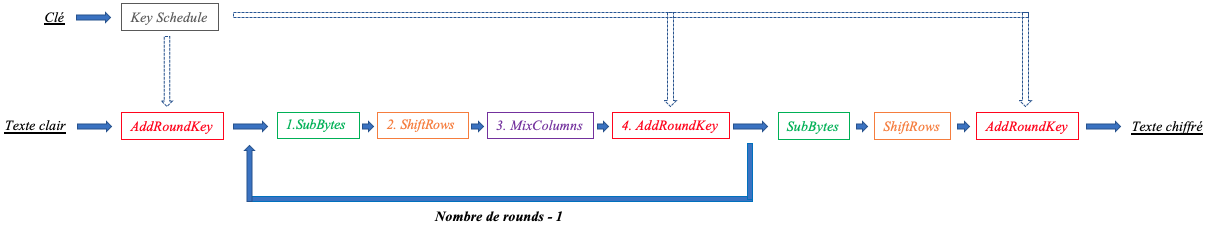
\includegraphics[scale=0.48]{image/AES_General}
    \caption{Fonctionnement général de l'algorithme AES.}
    \label{fig:AES_General}
\end{figure}

\newpage

L'AES-128 a donc pour rôle de chiffrer des blocs de données de 128 bits avec une clé de 128 bits. Les données et la clé sont représentées par une matrice où chaque élément de la matrice correspond à un byte (un octet, i.e 8 bits). Étant donné que 128 bits correspondent à 16 bytes, la matrice de données, au même titre que la matrice de clé, correspond à une matrice de 4 lignes et 4 colonnes (formant ainsi les 4x4 soit 16 bytes). Une matrice particulière (de taille 4x4 également) appelée STATE contient l'ensemble des résultats intermédiaires résultant des diverses opérations que subissent les données (depuis leur état initial). La figure \ref{fig:matrix} présente les 3 matrices qui viennent d'être citées : la matrice de données (message clair initial de 128 bits), la matrice STATE (qui va contenir les résultats intermédiaires des données suite aux différentes opérations) et la matrice clé (clé de 128 bits).
\begin{figure}[htbp]
    \centering
    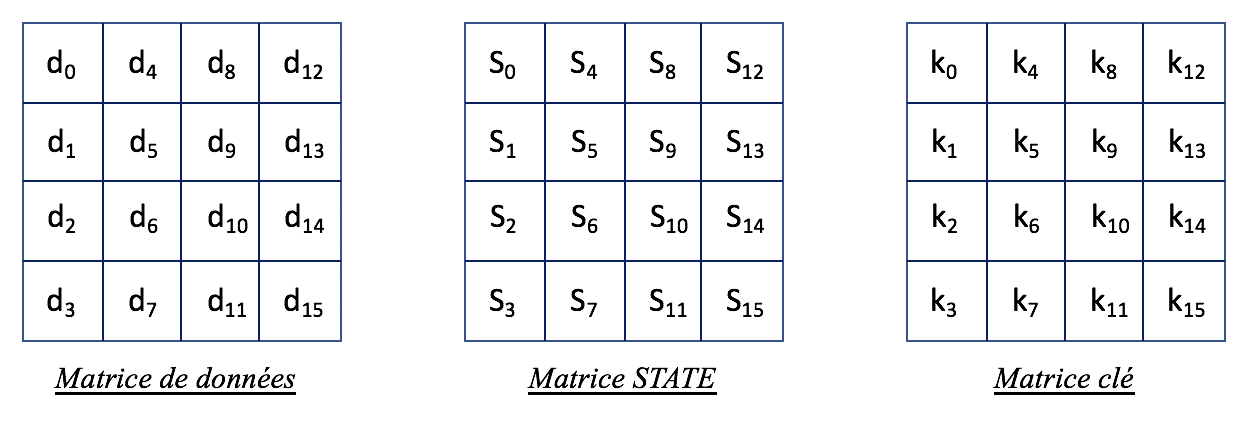
\includegraphics[scale=0.6]{image/matrix}
    \caption{Les 3 matrices utilisées par l'algorithme AES.}
    \label{fig:matrix}
\end{figure}

\hspace{-0.5cm}\textit{Remarque} : En pratique, la matrice de données est directement confondue avec la matrice STATE. Autrement dit, les premiers éléments à être placés dans la matrice STATE représentent les bytes de données. Ainsi, on n'utilise que deux matrices durant le fonctionnement de l'algorithme AES : la matrice STATE et la matrice clé.

\vspace{0.5cm}
\underline{\textbf{Fonctionnement AES-128 :}} 

\hspace{-0.5cm}Initialement, deux matrices vont être utilisées : la matrice STATE, contenant les données claires, et la matrice clé, contenant la clé secrète initiale. Comme on peut le voir sur la figure \ref{fig:AES_General}, la première opération à être appliquée sur ces deux matrices est l'opération \textit{AddRoundKey}. Cette opération réalise un XOR (symbole \oplus) entre chaque élément de la matrice STATE et chaque élément respectif de la matrice clé. Le résultat est ré-écrit dans la matrice STATE. La figure \ref{fig:XOR} ci-dessous présente le principe de fonctionnement de cette première opération :
\begin{figure}[htbp]
    \centering
    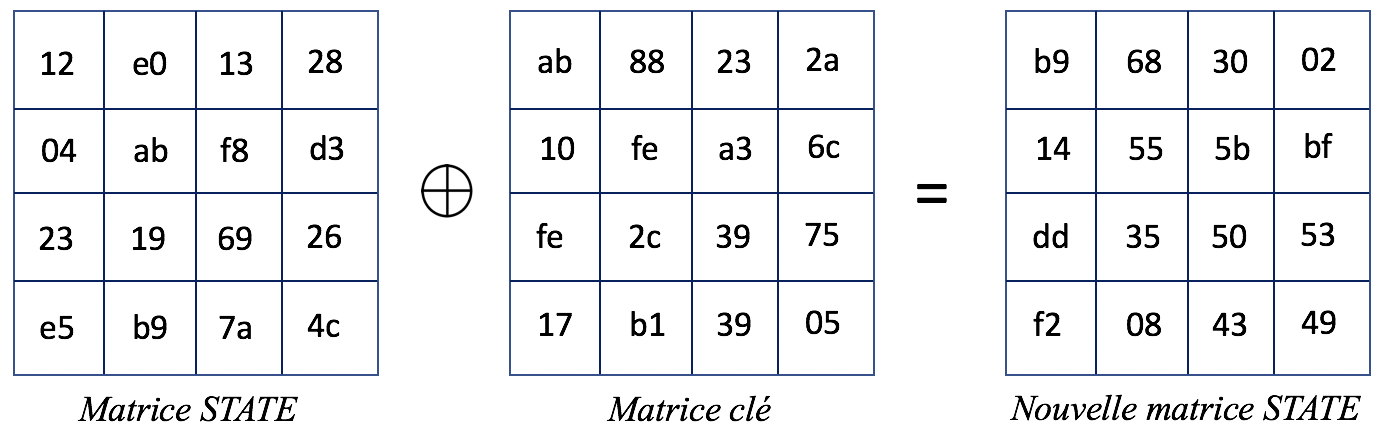
\includegraphics[scale=0.52]{image/XOR}
    \caption{Opération \textit{AddRoundKey} entre la matrice STATE et la matrice clé.}
    \label{fig:XOR}
\end{figure}

\hspace{-0.5 cm}Ensuite, toujours selon la figure \ref{fig:AES_General}, une série de quatre opérations se répétant neuf fois (car AES-128) est exécutée. Ces quatres opérations sont appliquées dans l'ordre chronologique suivant : \textit{SubBytes}, \textit{ShiftRows}, \textit{MixColumns}, \textit{AddRoundKey}. \\
Enfin, une fois les neufs rounds exécutés, trois opérations terminent le chiffrement : \textit{SubBytes}, \textit{ShiftRows} et \textit{AddRoundKey}. À la fin de ces trois dernières opérations, une matrice de taille 4x4 (la matrice STATE) présente le message chiffré de 128 bits.


\newpage
\underline{\textbf{Description des 4 opérations :}} \\
\begin{description}
\item[1. SubBytes]: La figure \ref{fig:SubBytes} ci-dessous présente le principe de fonctionnement de l'opération \textit{SubBytes}. Le principe de fonctionnement présenté dans ce cas-ci est simple : il repose sur une table de substitution, appelée Sbox et présentée en annexe \ref{ann:Sbox}. La matrice STATE avant l'exécution de l'opération contient 16 bytes. Chacun de ses 16 bytes (notés $S_{i,j}$) va fournir une nouvelle valeur de byte (noté $S'_{i,j}$) en fonction de la table de substitution. Un exemple est donné afin de comprendre le principe : Si le byte $S_{1,2}$ vaut $53$ (en hexadécimal) alors, selon la table Sbox, la valeur du byte résultant $S'_{1,2}$ vaut $ed$ (en hexadécimal).

\begin{figure}[htbp]
    \centering
    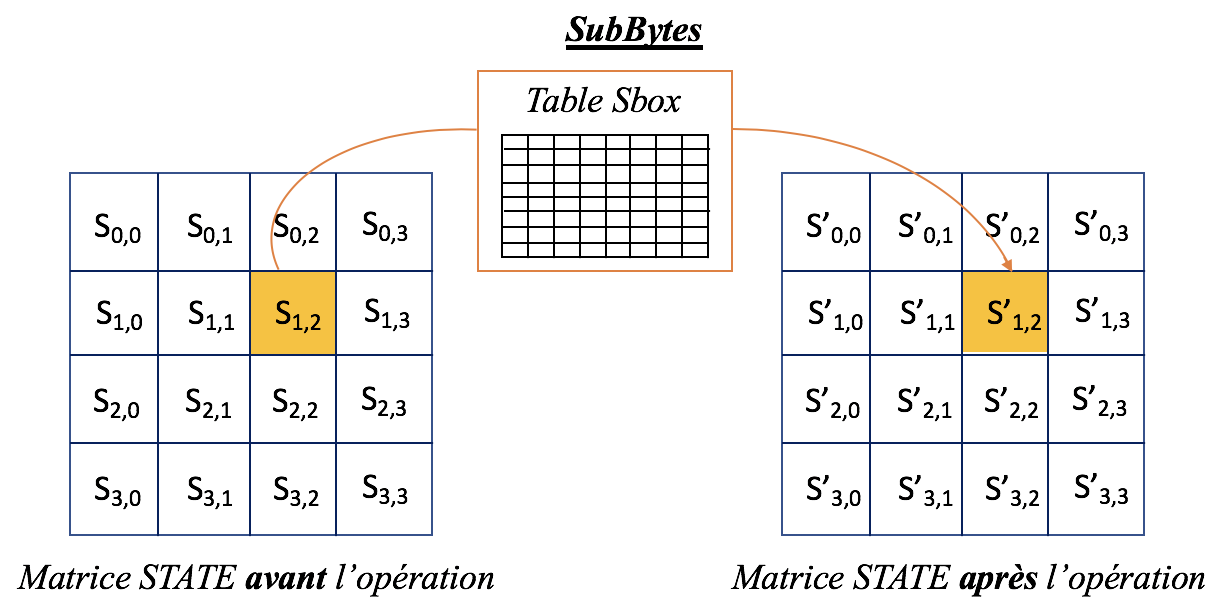
\includegraphics[scale=0.58]{image/SubBytes}
    \caption{Opération \textit{SubBytes} exécutée sur la matrice STATE.}
    \label{fig:SubBytes}
\end{figure}
\vspace{1cm}

\item[2. ShiftRows]: Comme son nom l'indique, cette opération concerne les lignes de la matrice STATE. Cette opération réalise une permutation cyclique des octets sur les lignes de la matrice STATE. Plus précisément, \textbf{pour la \textit{i-ième} ligne, on décalera chaque élément de la matrice STATE de \textit{i} positions vers la gauche}, en considérant que la première ligne a pour indice 0.
La figure \ref{fig:ligne} ci-dessous présente le principe de fonctionnement de l'opération \textit{ShiftRows} :
\begin{figure}[htbp]
    \centering
    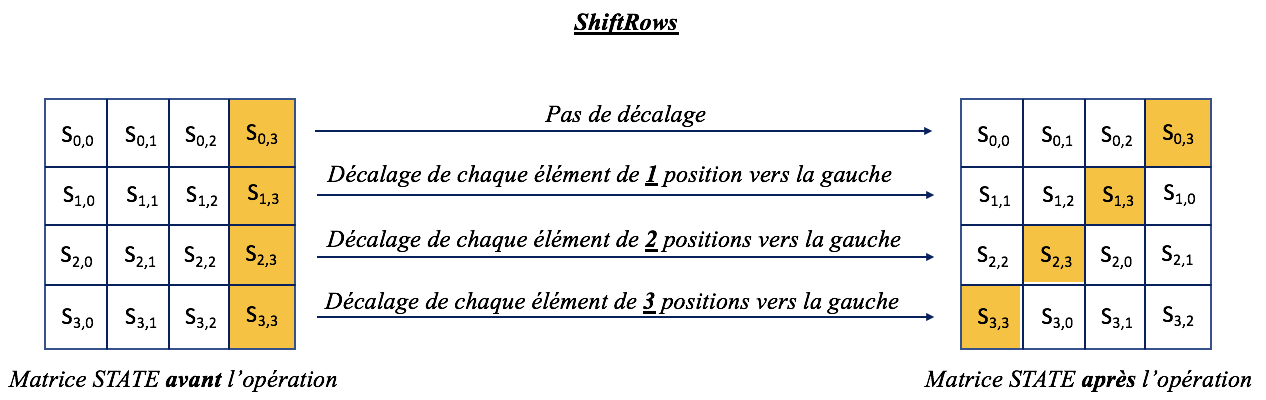
\includegraphics[scale=0.8]{image/ligne}
    \caption{Opération \textit{ShiftRows} exécutée sur la matrice STATE.}
    \label{fig:ligne}
\end{figure}

\newpage
\item[3. MixColumns] : Comme son nom nom l'indique, cette opération concerne les colonnes de la matrice STATE. \textbf{Cette opération réalise un produit matriciel entre une matrice fixée (taille 4x4) définie ci-dessous} (figure \ref{fig:colonnebis}) \textbf{et un vecteur colonne (taille 4x1) de la matrice STATE}. Il en résulte un nouveau vecteur colonne (taille 4x1) permettant de définir la nouvelle matrice STATE.
La figure \ref{fig:colonne} ci-dessous présente le principe de fonctionnement de l'opération \textit{MixColumns}. Un exemple est ensuite donné à la figure \ref{fig:colonnebis}.

\begin{figure}[htbp]
    \centering
    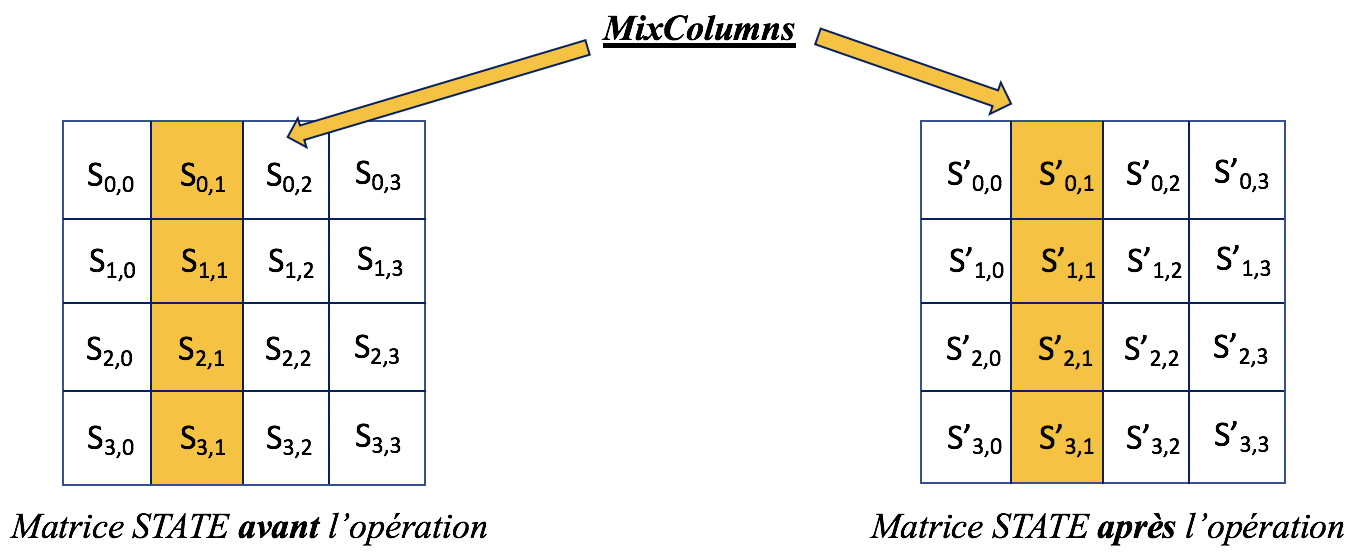
\includegraphics[scale=0.55]{image/colonne}
    \caption{Opération \textit{MixColumns} exécutée sur la matrice STATE.}
    \label{fig:colonne}
\end{figure}
\begin{figure}[htbp]
    \centering
    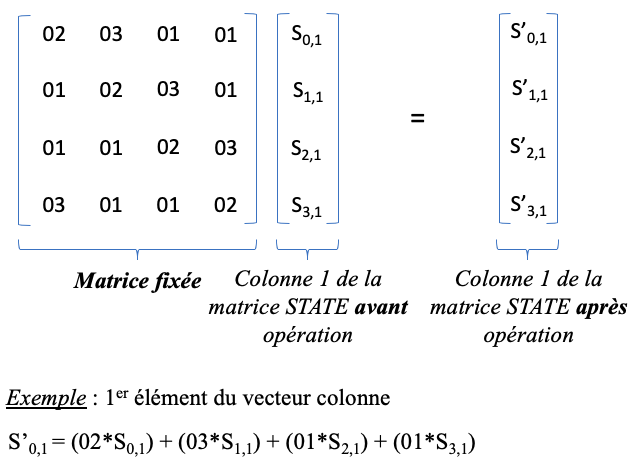
\includegraphics[scale=0.42]{image/colonnebis}
    \caption{Exemple de l'opération \textit{MixColumns} exécutée sur la deuxième colonne (i.e colonne 1) de la matrice STATE.}
    \label{fig:colonnebis}
\end{figure}
\vspace{1cm}

\item[4. AddRoundKey] : Comme précisé précédemment dans le fonctionnement initial, l'opération \textit{AddRoundKey} réalise un XOR entre la matrice STATE et la matrice de clé. Le résultat de ce XOR est placé dans la nouvelle matrice STATE (voir figure \ref{fig:XOR}).\\ 
\end{description}

\newpage
\underline{\textbf{L'opération \textit{KeySchedule} :}}

\vspace{0.1cm}Il persiste une opération qui n'a pas encore été expliquée : l'opération \textit{KeySchedule}. Cette opération s'exécute uniquement sur la matrice clé. Par conséquent, la gestion des clés se fait au travers des deux fonctions qui sont les fonctions \textit{AddRoundKey} et \textit{KeySchedule}. Nous connaissons le principe de fonctionnement de l'opération \textit{AddRoundKey}, reste à comprendre l'utilité de l'opération \textit{KeySchedule}.

\hspace{-0.5cm}Jusqu'à présent, nous avons vu que la matrice STATE était modifiée après chaque opération exécutée. Ce qu'on ne sait pas encore, c'est que la matrice clé est également modifiée à chaque round afin d'éviter d'utiliser toujours la même valeur de clé. Cela permet ainsi de complexifier le chiffrement des données. On l'aura deviné, l'opération qui modifie la matrice clé initiale en une nouvelle matrice clé est appelée \textbf{\textit{KeySchedule}}. Cette opération génère une nouvelle clé sur base de la clé précédemment employée. Ainsi, pour générer la première nouvelle clé, l'opération \textit{KeySchedule} emploiera la clé initialement donnée. Étant donné que pour l'AES-128, nous avons un total de dix rounds à exécuter, cela signifie que l'opération \textit{KeySchedule} s'exécute dix fois afin de générer dix nouvelles clés de 128 bits. En rajoutant la clé initiale, nous avons alors onze clés de chiffrement différentes permettant d'exécuter les onze opérations \textit{AddRoundKey} présentes dans l'algorithme AES-128. Ainsi, comme présenté à l'annexe \ref{ann:AES128}, l'opération \textit{KeySchedule} s'exécute en premier lieu dans le code afin de générer dix nouvelles clés. En comptant la clé initialement donnée, il y a donc onze clés. Chacune de ces onze clés sera utilisée lors de l'appel de la fonction \textit{AddRoundKey}. 

\hspace{-0.5cm}L'annexe \ref{ann:KeySchedule} permet de comprendre le principe de fonctionnement de l'opération \textit{KeySchedule}, utilisée afin de générer les nouvelles clés. Plus précisément, cette annexe présente un exemple pour générer la première nouvelle clé (taille de 128 bits). Le fonctionnement est le suivant : l'opération \textit{KeySchedule} s'exécute colonne par colonne sur la matrice clé de taille 4x4. On va d'abord générer la première colonne de la nouvelle clé, ensuite on générera les colonnes 2, 3 et 4. C'est la première colonne qui est la plus compliquée à générer. Les 3 autres colonnes réalisent simplement un XOR pour générer la nouvelle colonne.
Ainsi, pour obtenir la 1ère colonne de la nouvelle clé (soit les quatre premiers bytes), on va prendre trois vecteurs colonnes (taille 4x1), à savoir : 
\begin{enumerate}
\item Prendre la 4ème colonne de la clé initiale.
\begin{enumerate}
\item Décaler chaque élément de cette colonne d'une position vers le haut.
\item Appliquer l'opération \textit{SubBytes} sur chaque élément de la colonne.
\end{enumerate}
\item Prendre la 1ère colonne de la clé initiale.
\item Prendre la 1ère colonne de la matrice RCON.
\end{enumerate}
Une fois ces trois vecteurs colonnes obtenus, on réalise un XOR entre eux. Le résultat de ce XOR représente la 1ère colonne de la nouvelle matrice clé. Pour les colonnes 2, 3 et 4, le principe est le suivant : la colonne \textit{i} de la nouvelle clé est obtenue en réalisant un XOR entre la colonne \textit{i} de l'ancienne clé et la colonne \textit{i-1} de la nouvelle clé (avec $i$ {\epsilon} \{2 ; 4\}). L'annexe \ref{ann:KeySchedule} donne un exemple concret et didactique de l'opération \textit{KeySchedule}. \\

\underline{\textbf{Adaptation pour l'AES-256 :}} 

\vspace{0.1cm}En se basant sur le tableau \ref{tab:AES} et la figure \ref{fig:AES_General}, nous constatons que les deux différences majeures entre l'algorithme AES-128 et l'algorithme AES-256 sont :
\begin{itemize}
\item La taille de la clé : on passe de 128 bits à 256 bits.
\item Le nombre de rounds : on passe de 10 rounds à 14 rounds. \\
\end{itemize}
Ainsi, l'opération \textit{KeySchedule} s'exécute 14 fois. Cependant, cette opération ne génère pas 14 nouvelles clés de 256 bits mais seulement 7 nouvelles clés de 256 bits. La raison est la suivante : les 256 bits de la clé sont scindés en deux parties égales, c'est-à-dire en 128 bits, afin que les 4 autres opérations décrites précédemment (\textit{SubBytes}, \textit{ShiftRows}, \textit{MixColumns} et \textit{AddRoundKey}) puissent s'exécuter sans problème. En effet, la matrice STATE ayant toujours une taille de 128 bits, la matrice clé doit obligatoirement avoir une taille équivalente (128 bits) afin que les quatre opérations puissent être exécutées comme décrit pour l'algorithme AES-128. Le premier round utilisera donc les seize premiers bytes de la clé initiale ; Le second round utilisera les seize derniers bytes de la clé initiale (les trente-deux bytes de la clé initiale ont ainsi été utilisés) ; Le troisième round utilisera les seize premiers bytes de la seconde clé, générée par l'opération \textit{KeySchedule} ; et ainsi de suite jusqu'au quatorzième et dernier round.



\newpage

%%%%%%%%%%%%% Chapitre 3 %%%%%%%%%%%%%

\chapter{Consommation de puissance}
\label{chap:puissance}

Ce chapitre introduit au lecteur une technologie bien répandue dans les systèmes informatiques modernes : la technologie CMOS. C'est en étudiant le fonctionnement de cette technologie que les attaques par analyse de la consommation de puissance sont rendues praticables. Le principe de fonctionnement de cette technologie constitue donc une étape nécessaire dans l'apprentissage du lecteur. En effet, ce dernier sera ainsi en mesure de comprendre pourquoi une analyse de la consommation de puissance d'un circuit en technologie CMOS permettra plus tard (chapitre \ref{chap:attaques}) de retrouver la clé d'un algorithme de chiffrement. De cette façon, ce chapitre se scinde en deux parties. Dans un premier temps, l'objectif est de comprendre le fonctionnement de la technologie CMOS ainsi que ses répercussions sur les différentes puissances intervenant. Dans un second temps, l'objectif est d'assimiler le concept de \textit{modèle de puissance}. Pour ce faire, deux modèles seront judicieusement développés.

\section{Technologie CMOS}
\label{sec:CMOS}
La \textbf{\textit{technologie CMOS}} (pour \textit{Complementary Metal Oxyde Semiconductor}) est la technologie la plus répandue parmi toutes les technologies de semi-conducteurs. En effet, on la retrouve dans la majorité des systèmes informatiques modernes. En 2001, elle couvrait 86\% de la production mondiale des circuits intégrés. Pour cette raison, nous nous intéressons à leur conception afin de détecter des anomalies qui pourraient se révéler être utiles pour la cryptanalyse. \\
Le nom de cette technologie vient du fait que toutes les fonctions logiques (portes OR, AND, etc.) peuvent être réalisées moyennant l’utilisation d’une paire de transistors MOS complémentaires (N-MOS et P-MOS) associés symétriquement et fonctionnant en régime de commutation. Cela signifie que lorsqu'un des deux transistors MOS conduit, l’autre est par conséquent fermé. Grâce à ce principe, une porte logique CMOS ne consomme de l’énergie qu’au moment de la commutation. Cette caractéristique permet de distinguer le CMOS de toutes les autres technologies.

\hspace{-0.5 cm}Pour expliquer le fonctionnement de cette technologie, on peut prendre un exemple simple : \textbf{\textit{l'inverseur CMOS}}. Un inverseur CMOS est une fonction "\textit{NON}" dont voici la table de vérité (table \ref{tab:verite}):
\begin{table}[htbp]
	\centering
	\begin{tabular}{|c|c|}
    		\hline
   		  \textit{Entrée} & \textit{Sortie} \\ \hline 
   		  0 & 1 \\ 
   		  1 & 0 \\ \hline
	\end{tabular}
    	\caption{Table de vérité pour la fonction NON (inverseur CMOS).}
    	\label{tab:verite} 
\end{table}

\newpage

\hspace{-0.5 cm}La figure \ref{fig:CMOS} ci-dessous (schéma a) présente le schéma de l'inverseur CMOS :
\begin{figure}[htbp]
    \centering
    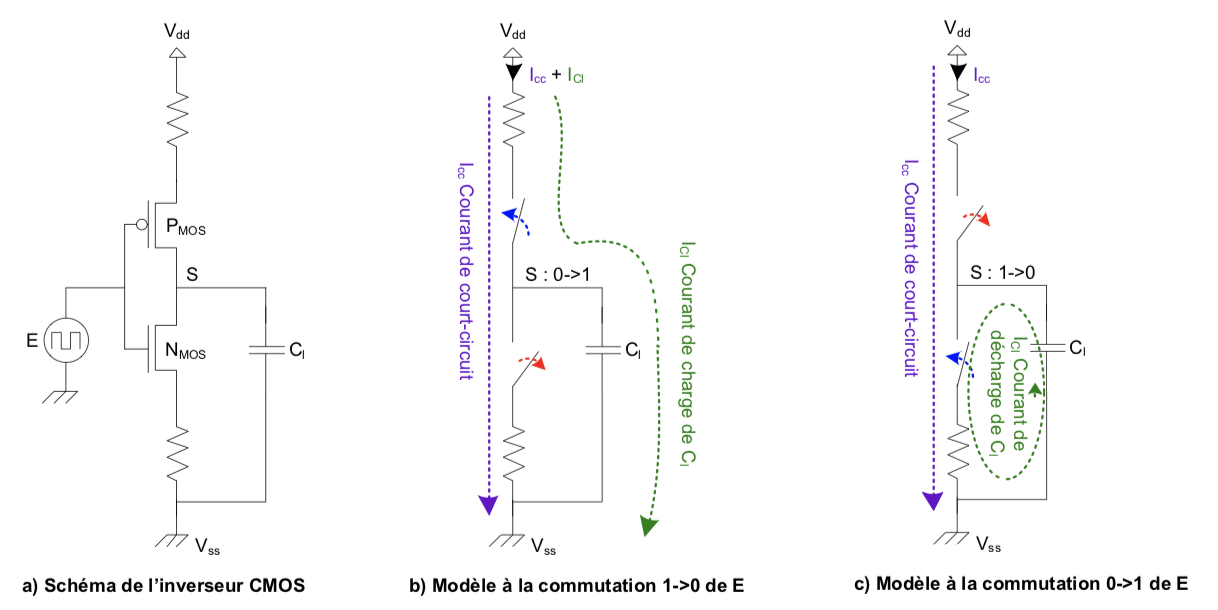
\includegraphics[scale=0.75]{image/CMOS}
    \caption{Schéma de l'inverseur CMOS.}
    \label{fig:CMOS} 
\end{figure}

Si on applique à l'entrée (E) un état bas, le transistor N est bloqué et le P est passant (schéma b). On place ainsi la sortie au potentiel Vdd (la tension d'alimentation), c'est-à-dire à l'état haut. Inversement, quand on met l'entrée à l'état haut, le transistor P est bloqué et le N est passant (schéma c). La sortie est donc à l'état bas. On a donc bien réalisé une fonction inversion. Dans la suite de ce travail, on considérera toujours que les circuits attaqués sont réalisés en technologie CMOS.


\subsection{Consommation de puissance des circuits en technologie CMOS}
\label{sec:puissance}

Il est évident que les circuits digitaux modernes consomment de la puissance lorsqu'ils exécutent des instructions. Dans notre cas, c'est un FPGA sur lequel est implémenté l'algorithme AES qui consomme de la puissance. Dans le domaine de la cryptanalyse, cette puissance va être mesurée et analysée afin de déterminer si le device cryptographique laisse fuiter des informations. Si tel est le cas, nous verrons comment ces informations peuvent être utilisées afin de retrouver la clé de chiffrement de l'algorithme AES (chapitre \ref{chap:attaques}). Pour ce faire, nous devons tout t'abord étudier les différentes puissances intervenant dans les circuits réalisés en technologie CMOS. Pour rappel, cette technologie est très répandue et couvre la plupart des circuits digitaux modernes. 

La consommation totale de puissance d'un circuit CMOS peut être obtenue en sommant les consommations de puissance respectives de chaque cellule logique (cellule conçue pour remplir une certaine fonction logique) du circuit CMOS. De cette façon, la consommation de puissance totale dépend essentiellement du nombre de cellules logiques dans le circuit CMOS. \\
En prenant comme exemple de cellule logique CMOS, l'inverseur CMOS (expliqué à la section \ref{sec:CMOS}), nous allons tenter de comprendre quand et pour quelles raisons ces cellules CMOS dissipent de la puissance. Pour ce faire, il faut savoir que la consommation de puissance est essentiellement divisée en deux parties : 
\begin{itemize}
\item La puissance statique (notée $P_{stat}$): C'est la puissance qui est consommée lorsqu'il n'y a pas de commutation dans une cellule (c'est-à-dire dans l'inverseur). Autrement dit, c'est la puissance qui est consommée lorsque l'inverseur est en fonctionnement normal mais ne commute pas.
\item La puissance dynamique (notée $P_{dyn}$) : C'est la puissance qui est consommée par une cellule si la sortie de celle-ci commute. 
\end{itemize}
Ainsi, la puissance totale consommée par une cellule vaut la somme de ces deux composantes, soit :
\begin{gather}
	P_{total} = P_{stat} + P_{dyn}
\end{gather}

Mais de façon plus précise, que vaut la puissance statique ? De même, comment peut-on exprimer la puissance dynamique ? 

\hspace{-0.5 cm}\underline{\textbf{\textit{Puissance statique :}}} \vspace{0.2 cm} \\
Les cellules CMOS sont toujours construites de façon à ce que les deux transistors complémentaires ne soient jamais passants au même moment. En effet, si on reprend l'exemple de l'inverseur CMOS (\ref{sec:CMOS}), lorsqu'on met le signal d'entrée à \textit{GND} alors le transistor P1 est passant et N1 est bloqué. Par contre, lorsqu'on met le signal d'entrée à \textit{$V_{DD}$}, le transistor P1 devient bloqué tandis que le transistor N1 devient passant. Ainsi, en théorie, un seul transistor fonctionne et laisse passer du courant. Cependant, en pratique, lorsqu'un transistor MOS est bloqué, le courant qui le traverse n'est jamais entièrement nul. En effet, une très petite valeur de courant circule dans le canal du transistor. Ce courant, que l'on appelle \textit{courant de fuite} et que l'on note \textit{$I_{fuite}$}, produit une consommation de puissance \textbf{statique} pouvant être calculée de la façon suivante :
\begin{gather}
	P_{stat} = I_{fuite} . V_{DD}
\end{gather}

\hspace{-0.5 cm}\fbox{
\begin{minipage}{\textwidth}
Ainsi, on peut conclure que la consommation de puissance statique des circuits CMOS correspond à la puissance qui est consommée par le circuit lorsqu'il n'y a pas de commutation dans une cellule. Cette puissance est typiquement très faible et sera, en pratique, négligée.
\end{minipage}
}
\vspace{0.6 cm} \\
\hspace{-0.5 cm}\underline{\textbf{\textit{Puissance dynamique :}}} \vspace{0.2 cm} \\
La consommation de puissance dynamique apparait typiquement lors d'une commutation des transistors. Une commutation est le passage d'un état haut à un état bas ou d'un état bas à un état haut. En réalité, il existe 4 transitions d'état possibles. Ces 4 possibilités sont reprises dans le tableau \ref{fig:dyn} ci-dessous. 
\begin{table}[htbp]
	\centering
	\begin{tabular}{|c|c|}
    		\hline
   		  \textit{Transitions} & \textit{Type de puissance consommée} \\ \hline 
   		  0  \rightarrow 0 & Statique \\ 
   		  0  \rightarrow 1 & Statique + Dynamique \\ 
		  1  \rightarrow 0 & Statique + Dynamique \\ 
   		  1  \rightarrow 1 & Statique \\ \hline
	\end{tabular}
    	\caption{Type de puissance consommée par une cellule CMOS en fonction des 4 transitions d'état de sa sortie.}
    	\label{fig:dyn} 
\end{table}

\hspace{-0.5 cm}On constate que pour chaque transition possible, il y a présence de puissance statique. Cependant, il n'y a présence de puissance dynamique que dans le cas d'une commutation, c'est-à-dire lors des deux transitions : 0\rightarrow1 et 1\rightarrow0.  En toute logique, la consommation de puissance totale dépend du type de cellule et de la technologie employée. Cependant, en général, on constate que : 
\begin{itemize}
\item \textbf{\textit{Lorsqu'il n'y a pas de commutation}} (transitions 0\rightarrow0 et 1\rightarrow1), la puissance totale reste plus ou moins constante. En effet, la puissance dynamique étant nulle, on ne retrouve dans le calcul de puissance totale que la puissance statique. Autrement dit : $P_{total}=P_{stat}$.
\item \textbf{\textit{Lorsqu'il y a une commutation}} (transitions 0\rightarrow1 et 1\rightarrow0), la puissance totale augmente. En effet, en plus de la puissance statique déjà présente, vient s'ajouter la puissance dynamique. Autrement dit : $P_{total}=P_{stat}+P_{dyn}$.
\end{itemize}

\vspace{+0.5 cm}\hspace{-0.5 cm}\fbox{
\begin{minipage}{\textwidth}
Ainsi, on peut conclure que la consommation de puissance dynamique des circuits CMOS correspond à la puissance qui est consommée par le circuit lorsqu'il y a une commutation dans la cellule. Cette puissance constitue un facteur dominant dans la consommation de puissance totale. Il est donc primordial de pouvoir la calculer.
\end{minipage}
}

\newpage
\hspace{-0.5 cm}\underline{\textbf{\textit{Calcul de la puissance dynamique :}}} 
Le calcul de la consommation de puissance dynamique se divise en deux parties. Pour mieux comprendre pourquoi, reprenons l'exemple de l'inverseur CMOS.

\begin{enumerate}
\vspace{-0.2 cm}\item \textbf{\textit{Puissance moyenne de chargement de la capacité}} : La figure \ref{fig:CMOS} présente le schéma de l'inverseur CMOS lorsqu'il y a une commutation de sa sortie de l'état 0 à l'état 1 (schéma b) et lorsqu'il y a une commutation de sa sortie de l'état 1 à l'état 0 (schéma c). Pour rappel, le fonctionnement de l'inverseur est le suivant : Lorsque le signal d'entrée est à 1 (ou 0), le transistor du dessous est passant (ou bloqué) alors que celui du haut est bloqué (ou passant), la sortie est donc à 0 (ou 1). Maintenant, il faut regarder dans le cas d'une commutation à la sortie de l'inverseur CMOS. Si il y a une commutation de l'état 0 à l'état 1 en sortie (schéma b), l'inverseur dessine un courant provenant de l'alimentation ($V_{DD}$) et venant charger le condensateur $C_L$. Ce courant est appelé \textit{courant de charge}. À contrario, lors d'une commutation de l'état 1 à l'état 0, l'inverseur décharge le courant du condensateur $C_L$ vers la masse ($GND$). Ainsi, on constate bien que la commutation à la sortie de l'inverseur génère un courant qui produira une partie de la consommation de puissance dynamique. La consommation de puissance moyenne de chargement de la capacité durant un temps T peut être calculée de la façon suivante (\ref{eqn:charge}) :
\begin{gather}
	P_{chrg} = \frac{1}{T}\int_{0}^{T}p_{chrg}(t)dt=\alpha.f.C_{L}.V_{DD}^{2}\label{eqn:charge}
\end{gather}
Où :
\begin{itemize}
\item $p_{chrg}(t)$ représente la consommation de puissance de chargement instantanée de la cellule.
\item $\alpha$ est le facteur d'activité. Il correspond au nombre moyen de transitions (0-1) en sortie de la cellule à chaque coup de clock.
\item $f$ représente la fréquence de clock.
\item $C_L$ représente la valeur de capacité du condensateur.
\item $V_{DD}$ représente la tension positive de l'alimentation. \\
\end{itemize}


\vspace{-0.2 cm}\item \textbf{\textit{Puissance moyenne causée par les courants de court-circuit}} : En plus de la puissance moyenne de chargement de la capacité, il existe lors d'une commutation un bref instant, durant lequel les deux transistors conduisent le courant. Cela a pour effet de créer un court-circuit entre $V_{DD}$ en $GND$. Ce court-circuit va dissiper, le temps de son passage, de la puissance. La consommation de puissance moyenne qui est causée par les courants de court-circuit dans une cellule durant un temps T peut être calculée de la façon suivante (\ref{eqn:cc}) :
\begin{gather}
	P_{cc} = \frac{1}{T}\int_{0}^{T}p_{cc}(t)dt=\alpha.f.C_{L}.V_{DD}.I_{fuite}.t_{cc}\label{eqn:cc}
\end{gather}

Où : 
\begin{itemize}
\item $p_{cc}(t)$ représente la puissance de court-circuit consommée par la cellule.
\item $\alpha$ est le facteur d'activité. Il correspond au nombre moyen de transitions (0-1) en sortie de la cellule à chaque coup de clock.
\item $f$ représente la fréquence de clock.
\item $V_{DD}$ représente la tension positive de l'alimentation.
\item $I_{fuite}$ représente le courant de fuite causé par le court-circuit.
\item $t_{cc}$ représente le temps durant lequel le court-circuit se produit.
\end{itemize}

\end{enumerate}

\hspace{-0.5 cm}\fbox{
\begin{minipage}{\textwidth}
En conclusion, les devices cryptographiques modernes (comme le FPGA) possèdent deux composantes en puissance : 
\begin{itemize}
\item Une \textbf{\textit{puissance statique}} de faible valeur, requise pour garder le device en fonctionnement continu. Elle dépend du nombre de transistors dans la cellule. Elle est \textbf{négligée}.
\item Une \textbf{\textit{puissance dynamique}} de haute valeur, qui apparait lors d'une commutation. Elle dépend des opérations exécutées et des données manipulées. Elle n'est \textbf{pas négligée}.
\end{itemize}
Ceci nous conduit donc à l'équation suivante (\ref{eqn:puissance}) : 
\begin{gather}
	P_{total}=P_{stat}+P_{dyn}\cong P_{dyn} = P_{chrg} + P_{cc} \label{eqn:puissance}
\end{gather}
\end{minipage}
}

La figure \ref{fig:static_dynamic} ci-dessous présente deux mesures différentes de consommation de puissance prises à l'oscilloscope. Ces mesures ont été réalisées sur un FPGA implémentant l'algorithme AES-256. On y distingue la puissance statique seule (en bleu) de la puissance statique et dynamique (en orange). La courbe bleue a été enregistrée lorsque le FPGA était en attente de textes clairs, autrement dit il ne chiffrait rien (\Rightarrow puissance statique). La courbe orange a été enregistrée lorsque le FPGA chiffrait des données (\Rightarrow puissance statique et dynamique). On constate donc bien que la puissance statique est de très faible valeur comparativement à la puissance dynamique.
\begin{figure}[htbp]
    \hspace{-1cm}
    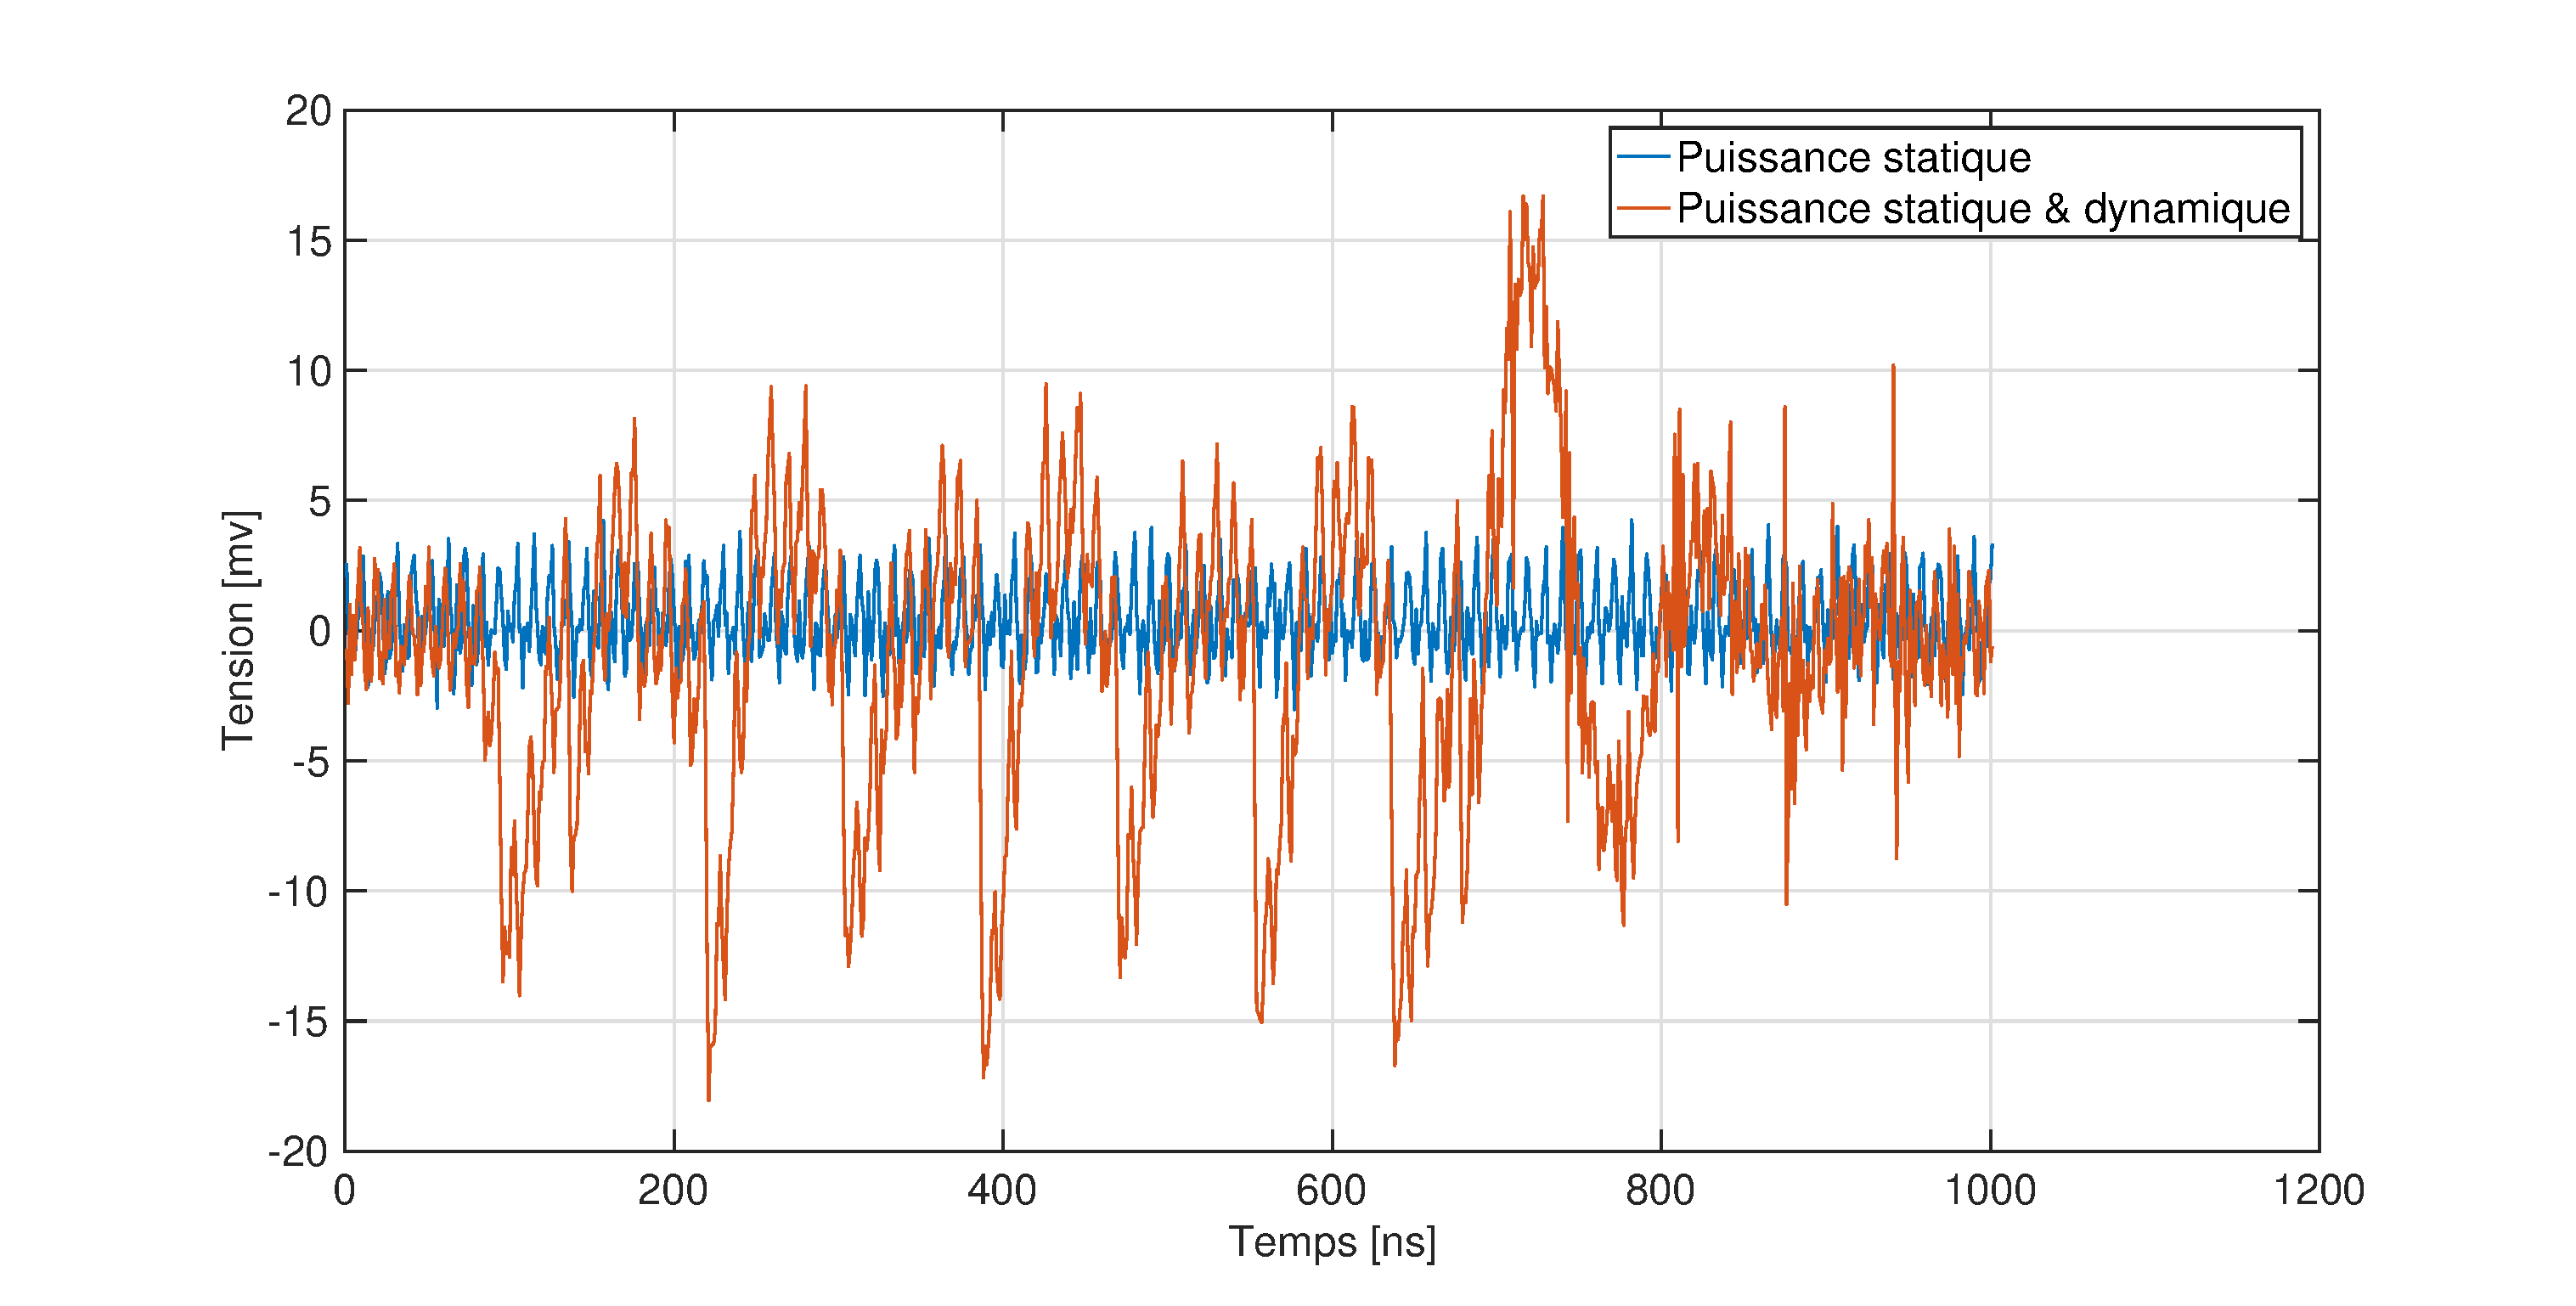
\includegraphics[scale=0.34]{image/static_dynamic}
    \caption{Comparaison de la puissance statique et dynamique.}
    \label{fig:static_dynamic}
\end{figure}



\vspace{-0.3cm}
\subsection{Composition des traces de puissance}
Les attaques basées sur l'analyse de la consommation de puissance exploitent le fait que la consommation de puissance d'un device cryptographique dépend des \textbf{opérations qu'il exécute} et des \textbf{données qu'il manipule}. Ces deux informations vont ainsi permettre de définir différentes propriétés intéressantes. Pour chaque point analysé dans une trace de puissance, on notera :
\begin{itemize}
\item \textbf{$P_{op}$ la composante dépendante de l'opération exécutée} ;
\item \textbf{$P_{data}$ la composante dépendante de la donnée manipulée}. \\
\end{itemize}
De plus, une troisième composante doit également être prise en compte. Cette composante fait référence au \textbf{bruit électrique} (aussi appelé bruit de fond) et sera notée \textbf{$P_{noise}$}. En effet, un signal est toujours affecté de petites fluctuations plus ou moins importantes. Ces fluctuations, dont les origines peuvent être diverses, sont appelées "bruit électrique" (ou simplement bruit). Le bruit est considéré comme un élément parasite aléatoire, c'est-à-dire qu'on ne sait pas le déterminer à l'avance. Au plus cette composante est élevée et au plus l'analyse de la consommation de puissance est difficile.

\hspace{-0.5cm}Ainsi, chaque point d'une trace de puissance peut être modélisé comme la somme des 3 composantes définies ci-dessus, soit : 
$P_{total} = P_{op} + P_{data} + P_{noise}$. Par ailleurs, en reprenant l'équation (\ref{eqn:puissance}) définie dans la section \ref{sec:puissance}, nous pouvons conclure que (équation \ref{eqn:conclusion}) :
\begin{gather}
	P_{total} = P_{op} + P_{data} + P_{noise} = P_{stat} + P_{dyn} \cong  P_{dyn} = P_{chrg} + P_{cc}\label{eqn:conclusion}
\end{gather}

En conclusion, la puissance consommée par un device cryptographique reflète directement ses activités internes. En effet, on remarque que cette puissance dépend aussi bien des opérations exécutées que des données manipulées, auxquelles il faut également ajouter la présence d'un bruit parasite inconnu (aléatoire). 



\section{Modèles de puissance}
\label{sec:modelpuissance}
Dans une attaque par analyse de la consommation de puissance, l'attaquant doit utiliser ce que l'on appelle un \textbf{modèle de puissance} afin de prédire la consommation de puissance du device cryptographique attaqué. Différents modèles de prédictions existent. Chacun de ces modèles se base sur les valeurs de bits dans des \textit{sets} de données. La qualité du modèle employé a un impact important sur l'efficacité de l'attaque. Deux modèles sont généralement définis et utilisés : Il s'agit des modèles de \textbf{Poids de Hamming} (\textit{Hamming Weight} - HW) et de \textbf{Distance de Hamming} (\textit{Hamming Distance} - HD). Il faut noter que ces deux modèles restent généraux, c'est-à-dire qu'ils ne requièrent pratiquement aucune connaissance à propos du design du circuit et sont par conséquent parfois imprécis. Une fois les prédictions obtenues, celles-ci sont comparées selon diverses méthodes (voir chapitre \ref{chap:attaques}) aux mesures réelles de consommation de puissance du device capturées à l'oscilloscope (traces de puissance). 

\subsection{Modèle de poids de Hamming}
\label{sec:modelHW}

Le poids de Hamming est le modèle de consommation de puissance le plus élémentaire. C'est celui le plus utilisé par un attaquant lorsqu'il s'agit d'estimer la consommation de puissance d'un circuit dont on ne connait pas certaines valeurs intermédiaires consécutives calculées durant l'exécution de l'algorithme. Ce modèle considère qu'un 0 ne mène à aucune quantité significative de consommation de puissance tandis qu'un 1 implique une quantité significative de puissance consommée. Ainsi, pour ce modèle, on assume que la consommation de puissance prédite est proportionnelle au nombre de bits à 1 d'une donnée traitée. Dit vulgairement, le poids de Hamming calcule le nombre de bits à 1 présents dans un nombre binaire. Mathématiquement, cela se traduit par l'expression \ref{eqn:HW} : \\
\begin{gather}
	HW(b_{0}) = \sum_{i=0}^{N-1} b_{0,i}\label{eqn:HW}
\end{gather}
Où $b_{0}$ est un mot de N bits. Par conséquent, $b_{0,i}$ est le $i^{ème}$ bit du mot binaire $b_{0}$. \\
\textit{Exemple} : $HW(100110) = 3.$

\subsection{Modèle de distance de Hamming}
\label{sec:modelHD}

La distance de Hamming est un modèle de consommation de puissance proposé par Brier et Al. Il est basé sur la relation entre la consommation de puissance et l'activité de commutation dans les circuits en technologie CMOS. En effet, comme indiqué en conclusion de la section \ref{sec:puissance}, la consommation de puissance d'un device en technologie CMOS est principalement d'ordre dynamique, c'est-à-dire due aux activités de commutation des cellules dans le circuit. Ainsi, ce modèle assume que la puissance totale consommée par un circuit CMOS (définie selon l'équation \ref{eqn:puissance}) est équivalente à la consommation de puissance lors de commutations (transitions 0 \rightarrow 1 et 1 \rightarrow 0). Ce modèle est donc proportionnel au nombre de transitions 0 \rightarrow 1 et 1 \rightarrow 0. La distance de Hamming entre 2 nombres binaires, $b_1$ et $b_2$ se calcule en comptant le nombre de transitions (0 \rightarrow 1 et 1 \rightarrow 0) entre ces 2 nombres, soit l'expression \ref{eqn:HD} : 
\begin{gather}
	HD(b_{1},b_{2}) = HW(b_1 \oplus b_2)\label{eqn:HD}
\end{gather}
\textit{Exemple} : $HD(110110,100100) = HW(110110 \oplus 100100) = HW(010010) = 2.$

\newpage

%%%%%%%%%%%%% Chapitre 4 %%%%%%%%%%%%%

\addtocontents{toc}{\protect\newpage}
\chapter{Attaques par canaux auxiliaires}
\label{chap:attaques}

Ce quatrième chapitre est sans conteste celui le plus attendu par le lecteur. Tout d'abord, une introduction générale est donnée au lecteur afin que ce dernier ait un aperçu des différentes possibilités d'attaques par canaux auxiliaires existantes. Ensuite, l'attention est plus particulièrement portée sur trois types d'attaques par analyse de la consommation de puissance, à savoir : les attaques par analyse simple de la consommation, les attaques par analyse différentielle de la consommation et les attaques par analyse de la consommation par corrélation. Nous noterons que l'attaque mise en oeuvre dans ce travail est celle d'analyse de la consommation par corrélation. Ultérieurement, le but sera ainsi d'attaquer l'implémentation de l'algorithme AES sur un FPGA. Les résultats de cette attaque seront présentés au chapitre X (Partie 2). 

\section{Introduction}
\label{sec:att}

\vspace{-0.1 cm}À la fin des années 1990, une nouvelle contrainte pour la conception de systèmes informatiques a vu le jour : la sécurité matérielle. Bien souvent, la sécurité d'un système informatique s'appuie plus sur les concepts \textit{software} que \textit{hardware}. Cependant, un nouveau mode d'attaque s'est développé. Il s'agit d'attaques physiques, c'est-à-dire d'attaques exploitant différents types d’information physique (consommation de puissance, rayonnement électromagnétique, temps de calcul, ...). Ces attaques posent un véritable problème à la théorie cryptographique. En effet, alors que les algorithmes de chiffrement utilisés dans des systèmes sécurisés sont habituellement considérés comme des éléments de confiance, la \textit{mise en œuvre} (implémentation) de ces algorithmes permet des attaques dévastatrices. En général, le but d'une attaque par canaux auxiliaires est de retrouver la clé de chiffrement utilisée par l'algorithme afin de déchiffrer des données sensibles. On distingue deux grandes familles d'attaques : 
\begin{itemize}
\item \textbf{\textit{Attaques invasives}} : Une attaque est dite invasive lorsque l'environnement interne du device cryptographique est manipulé et observé par l'attaquant. Accéder à l'environnement interne signifie accéder au \textit{silicon}. Ainsi, ce type d'attaque a généralement pour conséquence d'endommager voir de détruire entièrement le device cryptographique. La violation d'informations se fait donc au détriment du device. On distingue deux types d'attaques invasives : 
\begin{itemize}
\item Les attaques invasives \textbf{\textit{irréversibles}} qui conduisent à la destruction totale du device cryptographique. Ce type d'attaque est souvent réalisé pour connaître la conception physique d'un device. \textit{Exemple} : Découpage laser d’un circuit intégré.
\item Les attaques invasives \textbf{\textit{pseudo-réversibles}} qui n’entrainent pas forcément la destruction totale du device cryptographique, mais qui sont souvent tout de même invasives puisqu’elles nécessitent la préparation du circuit (découpe partielle du boitier du circuit intégré par exemple). Un exemple typique de ce type d'attaque est ce qu'on appelle les \textit{attaques en fautes}. Le principe consiste à manipuler les conditions environnementales du système (tension, température, lumière, \textit{clock}, etc.) pour générer volontairement des fautes. Les fautes ainsi créées peuvent entrainer le circuit dans des modes de fonctionnement conduisant à des erreurs et ces erreurs peuvent ensuite être exploitées pour déterminer la clé.
\end{itemize}
\item \textbf{\textit{Attaques non invasives}} : Une attaque est dite non invasive lorsqu'elle ne requière pas que le device cryptographique soit ouvert. Cette attaquant exploite ainsi l'analyse, en fonctionnement normal, d'informations s'échappant d'un device cryptographique. Cela peut être l'analyse de la consommation de puissance, l'analyse temporelle, l'analyse par rayonnement électromagnétique, etc... C'est ce type d'attaque qui sera étudié pour la réalisation de ce travail. \\
\end{itemize}

\hspace{-0.5 cm}La figure \ref{fig:attaques} ci-dessous présente les 3 ensembles d'attaques définis précédemment et donne pour chacun d'entre eux quelques exemples d'applications.
\begin{figure}[htbp]
    \hspace{-1.82 cm}
    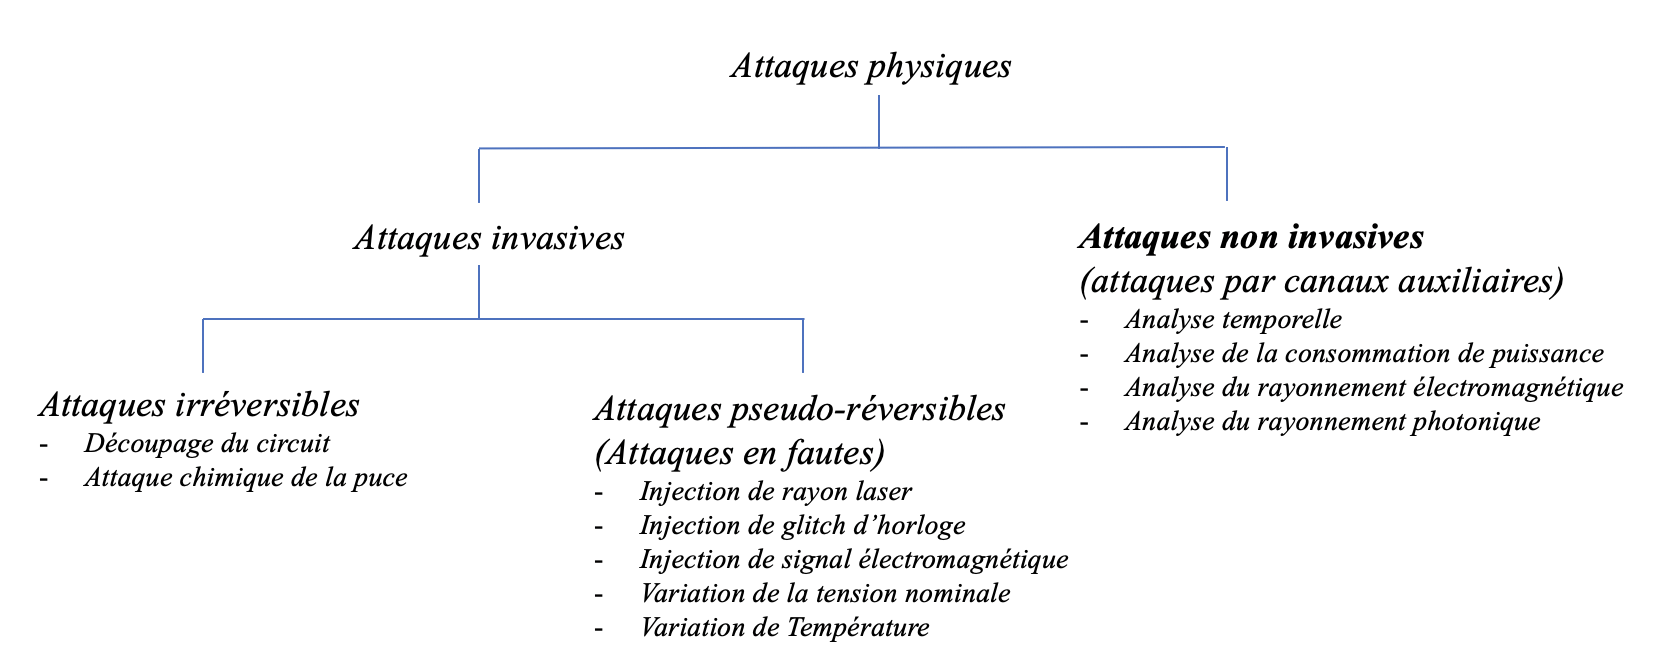
\includegraphics[width=1.19\textwidth]{image/attaques}
    \caption{Classification des attaques physiques.}
    \label{fig:attaques}
\end{figure}

\vspace{0.25 cm}Les attaques non invasives sont globalement beaucoup plus simples à mettre en oeuvre que les attaques invasives. En effet, du fait qu'il faille ouvrir le device cryptographique, les attaques invasives requièrent une méthodologie et une infrastructure relativement plus compliquée et plus chère que les attaques non invasives qui ne nécessitent pas de connaissances préalables du système interne et qui sont donc plus facilement déployées. 

\hspace{-0.5 cm}Les attaques non invasives consistent donc à analyser des données issues de canaux auxiliaires au device cryptographique lorsque ce dernier est en cours de chiffrement. Ces canaux auxiliaires sont des canaux présents physiquement sur le circuit attaqué et le long desquels de l’information s’échappe. Cette information peut se présenter sous différentes formes : rayonnement électromagnétique, rayonnement photonique, consommation de puissance, etc. C'est donc pour cette raison qu'on parle de \textit{side-channel attacks} ou en français \textit{l'attaque par canal auxiliaire}. 
En effet, les fonctions cryptographiques, bien que pouvant être extrêmement robustes théoriquement (c'est-à-dire mathématiquement) sont très sensibles aux fuites d’informations. C'est-à-dire qu'une quantité très faible d’informations peut être exploitée pour retrouver la clé d'un algorithme cryptographique très fort. On insistera à nouveau sur le fait que l'attaque exploite les faiblesses du système cryptographique, c'est-à-dire du système implémentant l'algorithme de chiffrement (l'AES en l'occurence). En aucun cas, l'attaque exploite les failles des principes mathématiques mis en place.

\newpage

\hspace{-0.5 cm}La figure \ref{fig:attackpassive} ci-dessous présente différentes possibilités \textbf{d'attaques non invasives} sur un device cryptographique.
\begin{figure}[htbp]
    \centering
    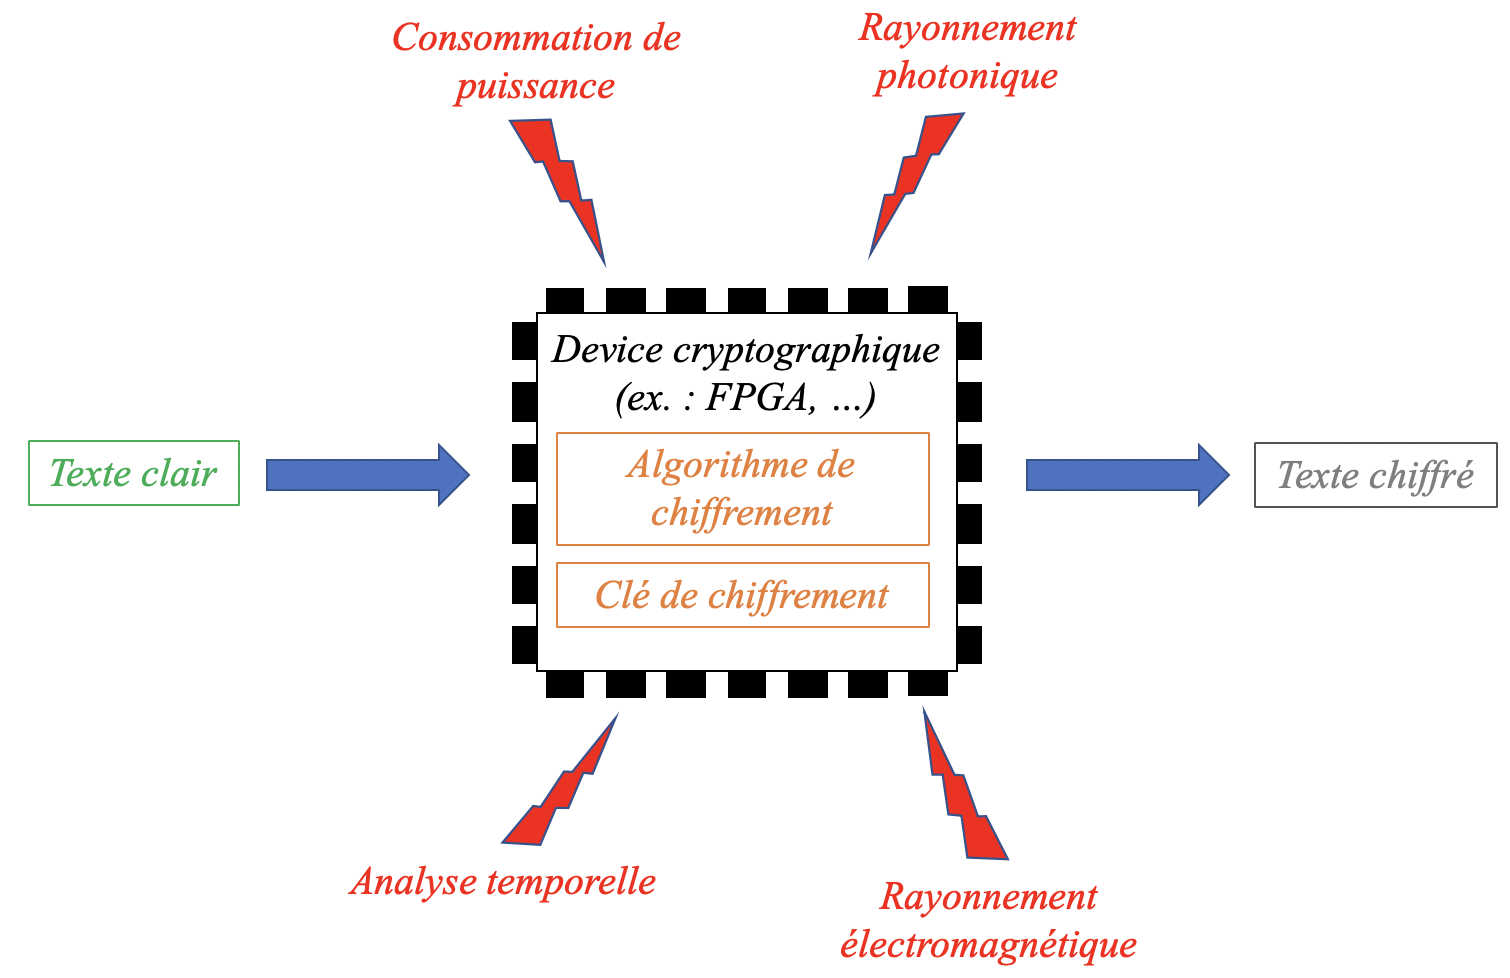
\includegraphics[scale=0.7]{image/attackpassive}
    \caption{Différentes façons d'opérer une attaque non invasive sur un device cryptographique.}
    \label{fig:attackpassive}
\end{figure}

Dans la suite de ce travail, on se concentrera sur un type précis d'attaque non invasive : l'attaque par \textbf{l'analyse de la consommation de puissance}. Les trois sous-sections de la section suivante (\ref{sec:PowerGeneral}) décrivent ainsi chacune un principe de fonctionnement différent d'attaque pour ce type d'analyse (consommation de puissance). L'attaque qu'il m'a été demandé de réaliser pour ce travail porte sur \textbf{l'analyse de la consommation par corrélation}. Pour cette raison, nous ne ferons que parcourir les deux autres possibilités que sont l'analyse simple de la consommation et l'analyse différentielle de la consommation. En effet, ces deux attaques sont apparues avant celle par corrélation et il convient donc de les citer pour que le lecteur comprenne l'ordre chronologique d'apparition et d'amélioration des attaques par analyse de la consommation.

\newpage

\section{Analyse de la consommation de puissance}
\label{sec:PowerGeneral}

La dénomination de l'attaque ne trompe pas : une attaque par analyse de la consommation de puissance a pour objectif d'analyser la consommation de puissance d'un device cryptographique en cours de chiffrement afin de retrouver la clé de l'algorithme implémenté sur ce device.

\subsection{Analyse simple de la consommation}
\label{sec:SPA}

Une analyse simple de la consommation (SPA en anglais pour \textit{Simple Power Analysis}) est une technique qui interprète directement la ou les mesure(s) de consommation capturée(s) sur un device cryptographique en cours de chiffrement. En d'autres mots, l'attaquant enregistre une trace de puissance et tente d'identifier sur celle-ci certaines opérations exécutées ou certaines données manipulées. En général, cela exige des connaissances avancées sur l'implémentation de l'algorithme cryptographique présent sur le device. Pour cette raison, ce type d'attaque est assez compliqué à réaliser en pratique même s'il n'exige qu'un nombre très limité de traces. Ainsi, ce type d'attaque permet en général d'identifier un algorithme cryptographique et dans des cas extrêmes et sous certaines conditions, il est même possible de lire la clé de chiffrement utilisée par l'algorithme.


\subsection{Analyse différentielle de la consommation}
\label{sec:DPA}

Une attaque par analyse différentielle de la consommation (DPA en anglais pour \textit{Differential Power Analysis}) est une attaque beaucoup plus populaire que l'attaque SPA. Ceci est dû au fait que l'attaque DPA ne requiert aucune connaissance approfondie sur le device cryptographique attaqué. De plus, cette attaque permet de retrouver la clé de chiffrement même si les traces capturées sont fortement bruitées. Par contre, en comparaison des attaques SPA qui tirent l'information d'un nombre restreint de traces, les attaques DPA nécessitent un plus grand nombre de traces et ce, afin de trouver des différences de consommation relatives à un bit. En effet, l’attaquant cherche à récupérer la clé de chiffrement en utilisant des informations relatives à un bit et en se basant sur un sous-ensemble de la clé et du texte (chiffré ou clair). Plus précisément, voici les quatre étapes utiles pour mettre en application une attaque DPA : 
\begin{enumerate}
\item \textbf{Mesurer la consommation de puissance} : l'attaquant doit mesurer et enregistrer des traces de puissance capturées sur le device cryptographique lorsque celui-ci est en cours de chiffrement. \textbf{Une trace} représente l'ensemble des opérations exécutées par un algorithme pour \textbf{un texte clair envoyé}. Étant donné qu'il faut un grand nombre ($N$) de traces pour que l'attaque DPA réussisse, il faudra par conséquent envoyer un grand nombre ($N$) de textes clairs.
\item \textbf{Modèle logiciel} : un modèle logiciel reproduit les opérations de l’algorithme implémenté et donne un résultat sur 1 bit pour chaque ensemble de clé testé. Prenons l'exemple de l'algorithme AES-128 pour mieux comprendre. Pour rappel, la clé utilisée par l'AES-128 a une taille de 128 bits. Si l'attaquant tente de retrouver un seul octet de la clé, c'est-à-dire 8 bits, il existe au total $2^{8}$ soit 256 valeurs possibles de clé. L'objectif de l'attaquant consistera à utiliser un modèle logiciel simulant l'algorithme AES-128 et testant les 256 clés possibles. L'attaque DPA fonctionne plus rapidement (moins de traces nécessaires) à la sortie de l'opération \textit{SubBytes} (par rapport aux trois autres opérations). Pour cette raison, le modèle logiciel reproduit les deux premières étapes de l’AES et donne un résultat sur 1 bit pour chacune des 256 sous-clés possibles. Ce résultat est un des bits en sortie de l’étape \textit{SubBytes}, le premier est couramment utilisé.
\item \textbf{Classement} : nous avons d'une part un ensemble de $N$ traces (disons 1000) et d'autre part un ensemble de bits de sélection (disons 256, soit pour 1 octet de la clé). Le but de l'attaquant est de classer les traces mesurées en deux groupes $G_0$ et $G_1$. La prise de décision se fait de la manière suivante : pour un texte clair $T_i$ avec $i \ \epsilon \ (0 \ ;1000)$, si le bit de sélection vaut 0 pour une clé $K_j$ avec $j \ \epsilon \ (0 \ ; 256)$, la trace de puissance $TP_i$ avec $i \ \epsilon \ (0 \ ; 1000)$ correspondant à ce texte clair $T_i$ est mémorisée dans un groupe $G_0$. À l'inverse, si le bit vaut 1, elle est mémorisée dans un groupe $G_1$.
\item \textbf{Mesurer la courbe DPA} : la différence de la moyenne temporelle des traces du groupe $G_1$ avec la moyenne temporelle des traces du groupe $G_0$ pour la sous-clé $K_j$ donne la courbe DPA associée à cette sous-clé. Il existe donc 256 courbes DPA (dans le cas où on souhaite retrouver un byte de la clé). Parmi celles-ci, la courbe dont la valeur moyenne est la plus élevée correspond à la clé de chiffrement.
\end{enumerate}

\hspace{-0.5 cm} La figure \ref{fig:DPA} ci-dessous présente les quatre étapes utiles pour mettre en oeuvre une attaque DPA.
\begin{figure}[htbp]
    \hspace{-1cm}
    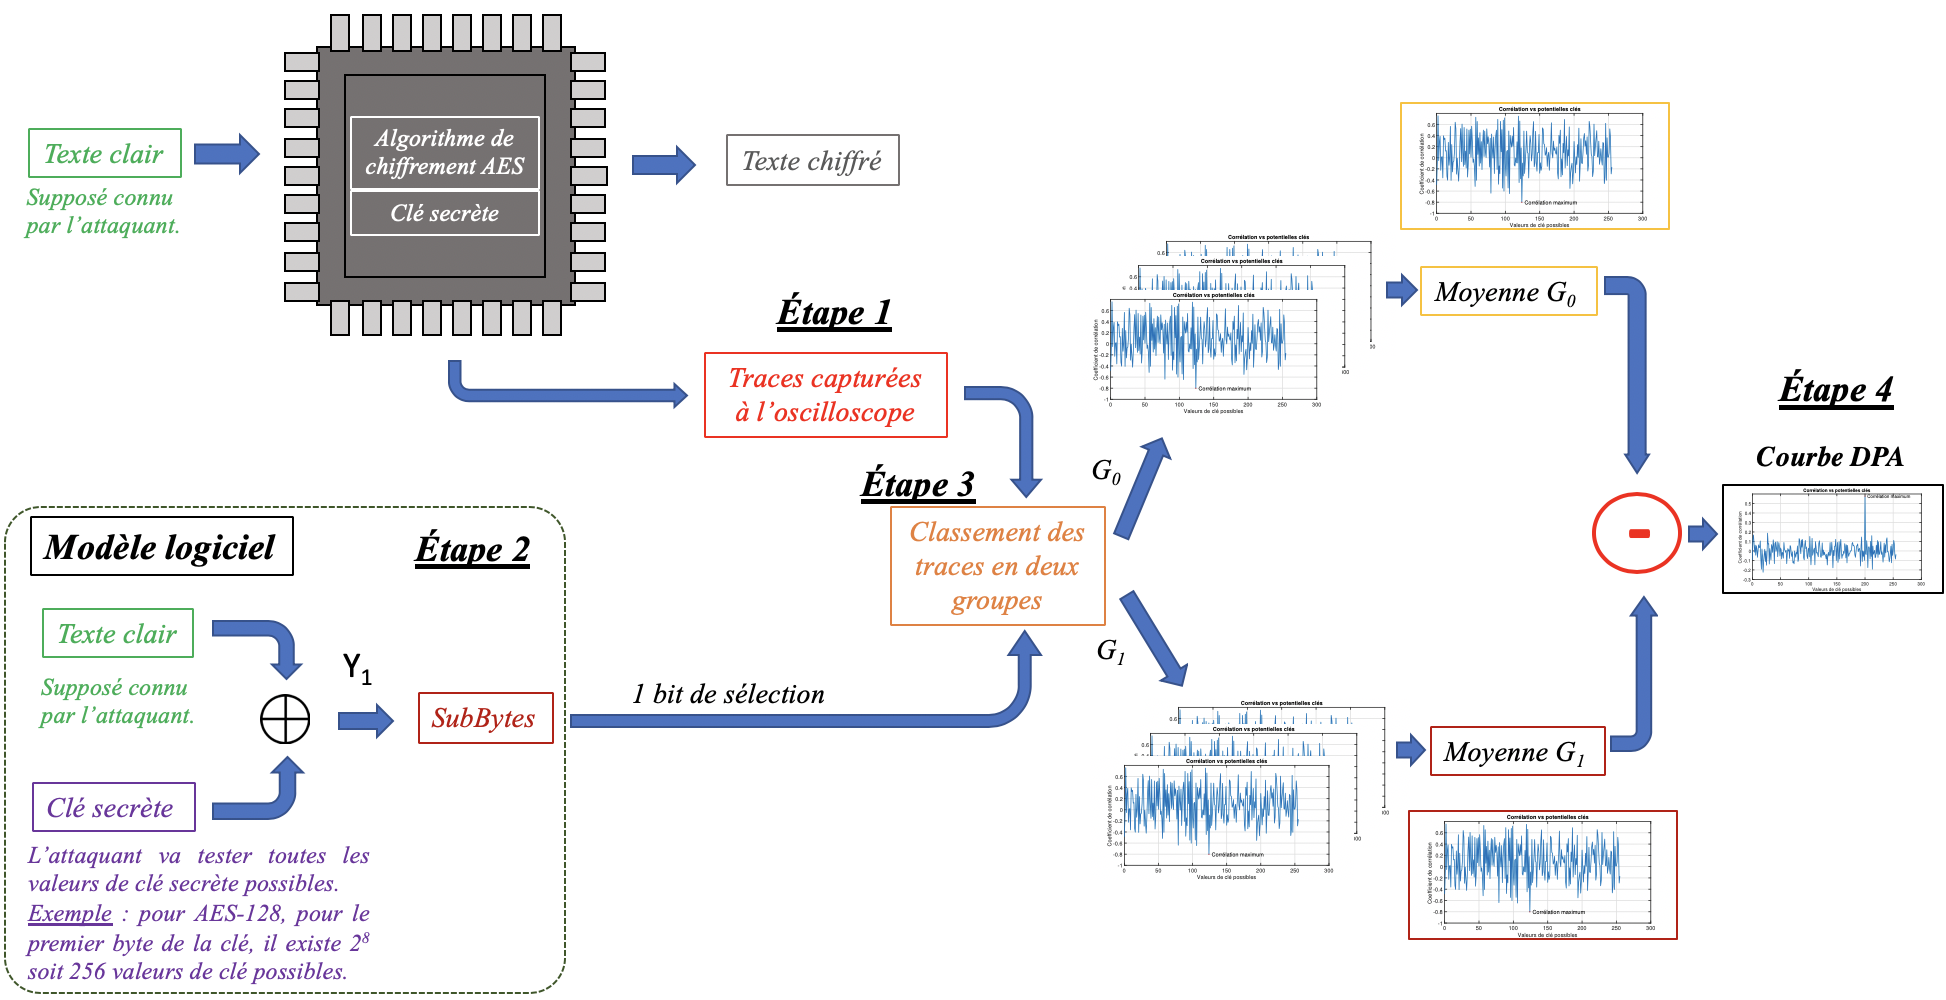
\includegraphics[scale=0.47]{image/DPA}
    \caption{Principe de fonctionnement d'une attaque DPA.}
    \label{fig:DPA}
\end{figure}


\subsection{Analyse de la consommation par corrélation}
\label{sec:CPA}

L'attaque par analyse de la consommation par corrélation (CPA en anglais pour \textit{Correlation Power Analysis}) est une attaque qui dérive de l’attaque DPA. En réalité, il s'agit d'une amélioration de l'attaque DPA. En effet, en 2004, de nouvelles recherches eurent pour objectif de directement calculer la corrélation entre la consommation de puissance du device cryptographique (les traces) et un modèle de prédiction de puissance (décrit à la section \ref{sec:modelpuissance}). La faille utilisée est la corrélation, dans les circuits électroniques de technologie CMOS, entre la consommation de puissance dynamique et le nombre de transistors qui commutent (de 0\rightarrow1 et de 1\rightarrow0) (voir chapitre \ref{chap:puissance}). Pour bien comprendre le fonctionnement de cette attaque, il convient donc de définir le terme \textit{corrélation} et plus précisément le terme \textit{coefficient de corrélation}.

\theoremstyle{definition}
\begin{definition}{\textbf{Coefficient de corrélation :}}
Par définition, le coefficient de corrélation est un coefficient statistique permettant de mettre en évidence une liaison entre deux types de séries de données statistiques. La valeur du coefficient de corrélation est toujours comprise entre -1 et 1. Cette valeur se calcule de la façon suivante (\ref{eqn:formcorrelation}) :
\begin{gather}
	r(X;Y) = \frac{\sum(X-\bar{X}).(Y-\bar{Y}) }{\sqrt{\sum(X-\bar{X})^2}.\sqrt{\sum(Y-\bar{Y})^2}}\label{eqn:formcorrelation}
\end{gather}
Où 
\begin{itemize}
\item $X$ et $Y$ sont deux séries de données statistiques.
\item $\bar{X}$ et $\bar{Y}$ sont les moyennes respectives des variables X et Y.\vspace{0.4 cm}
\end{itemize}
\end{definition}

\vspace{-0.4cm}\hspace{-0.5 cm}Sur base de la valeur du coefficient de corrélation, on peut conclure que :
\begin{itemize}
\item Si la valeur absolue du coefficient de corrélation est élevée (proche de 1), il y a une forte liaison entre les deux séries analysées.
\item Si la valeur absolue du coefficient de corrélation est faible (proche de 0), il y a une très faible liaison, voire aucun lien entre les deux séries analysées.
\end{itemize}

\hspace{-0.5 cm}Pour réaliser une attaque CPA, l'attaquant a principalement besoin de deux outils :
\begin{itemize}
\item \textbf{Un oscilloscope} : L'oscilloscope est utilisé pour enregistrer des traces de puissance sur le device attaqué. C'est-à-dire des mesures de tension en fonction du temps représentant la consommation de puissance du device cryptographique lorsque celui-ci chiffre un texte clair. $N$ textes clairs mènent à $N$ traces.
\item \textbf{Un ordinateur} : L'ordinateur est utilisé pour réaliser toute une série de calculs. Plus précisément, il réalise trois grands types de calculs : calculs d'opérations de l'algorithme de chiffrement (l'AES en l'occurence), calculs de prédiction de puissance (selon le modèle de puissance établi) et calculs des coefficients de corrélation. \\
\end{itemize}

Comme précisé ci-avant, l'oscilloscope est utilisé afin de capturer et d'enregistrer des données, appelées \textit{traces}, mesurées à partir des canaux auxiliaires du circuit électronique (dans notre cas, un FPGA). Pour réaliser la mesure à l'oscilloscope, une résistance est placée en série avec le canal (la PIN) connecté à la tension d'alimentation $V_{DD}$ du device cryptographique. L'oscilloscope est alors en mesure d'enregistrer une différence de potentielle $V(t)$ aux bornes de la résistance. Étant donné que le courant $I_{DD}(t)$ circulant dans le device cryptographique est de très faible valeur (\si{\micro}A), la tension $V(t)$ est également très faible. Ainsi, un amplificateur est généralement utilisé afin d'amplifier cette différence de potentielle. Comme nous le verrons au chapitre \ref{chap:config}, la \textit{board} de test employée (\textit{SAKURA-G}) utilise également un amplificateur pour mesurer une tension raisonnable. La figure \ref{fig:oscillo} ci-dessous présente le principe de mesure à l'oscilloscope.
\begin{figure}[htbp]
    \centering
    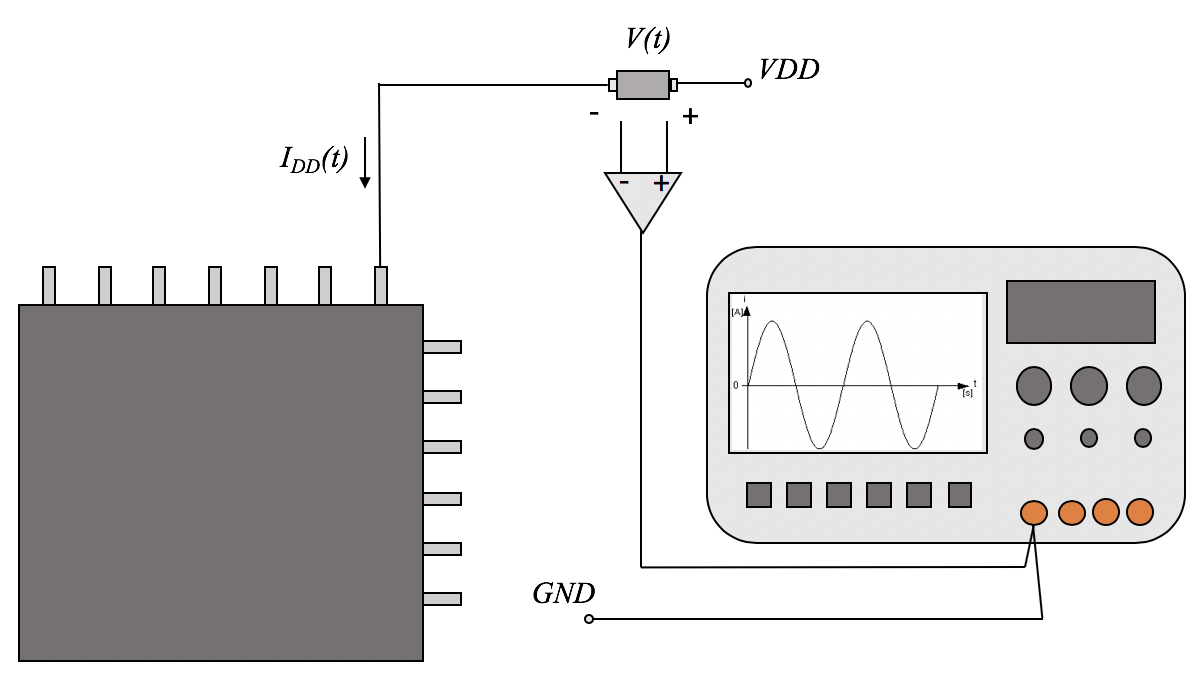
\includegraphics[scale=0.5]{image/oscillo}
    \caption{Principe de mesure à l'oscilloscope.}
    \label{fig:oscillo} 
\end{figure}

On parle d'attaque par analyse de la consommation de puissance or avec un oscilloscope, on mesure une tension et non une puissance. Cependant, comme le démontre l'équation \ref{eqn:oscillo}, la puissance consommée $p(t)$ est proportionnelle à la tension consommée $V(t)$. Il ne s'agit donc pas d'une erreur de parler de consommation de puissance. En effet, en supposant que la tension d'alimentation $V_{DD}$ est constante et par simple application de la loi d'Ohm, on a :
\begin{gather}
	\left\{\begin{matrix}
	u(t) = V_{DD}\\ 
	i(t) = \frac{V(t)}{R}
	\end{matrix}\right.
	\intertext{En reprenant la définition de la puissance consommée et en y remplaçant les termes $u(t)$ et $i(t)$, on a :}
	p(t) = u(t).i(t) = V_{DD}.\frac{V(t)}{R} \label{eqn:oscillo}
\end{gather}

\newpage

\hspace{-0.5 cm}Quatre étapes (similaires à l'attaque DPA) sont nécessaires à l'attaquant pour mettre en place une attaque CPA : 
\begin{enumerate}
\item \textbf{Mesurer la consommation de puissance} : l'attaquant doit mesurer et enregistrer des traces de puissance capturées sur le device cryptographique lorsque celui-ci est en cours de chiffrement. Une trace représente l'ensemble des opérations exécutées par un algorithme pour un texte clair envoyé. Étant donné qu'il faut un grand nombre ($N$) de traces pour que l'attaque CPA réussisse, il faudra par conséquent envoyer un grand nombre ($N$) de textes clairs.
\item \textbf{Calculer les valeurs intermédiaires hypothétiques} : comme nous l'avons vu au chapitre \ref{chap:crypto} section \ref{sec:algo}, lorsque l'algorithme AES chiffre des données, des valeurs intermédiaires sont calculées en fonction des opérations exécutées et des données manipulées. Prenons l'exemple de l'algorithme AES-128 pour bien comprendre. La clé utilisée a une taille de 128 bits. Si on tente de retrouver un seul octet de la clé, c'est-à-dire 8 bits, il existe au total $2^{8}$ soit 256 valeurs de clé possibles. L'objectif de l'attaquant va alors être de simuler l'algorithme AES-128 en testant les 256 clés possibles. Comme pour l'attaque DPA, l'attaque CPA fonctionne plus rapidement (moins de traces nécessaires) à la sortie de l'opération \textit{SubBytes} (par rapport aux trois autres opérations). Pour cette raison, la simulation sur ordinateur reproduit les deux premières étapes de l’AES et donne un résultat sur 8 bits pour chacune des 256 sous-clés possibles. Nous noterons qu'il est envisageable de réaliser l'attaque en sortie d'une des trois autres opérations de l'AES (\textit{AddRoundKey}, \textit{ShiftRows} ou \textit{MixColumns}). Cependant cela nécessiterait d'envoyer plus de messages clairs, d'enregistrer plus de traces et par conséquent, cela prendrait plus de temps. Il s'agirait donc d'une attaque non optimisée.
\item \textbf{Utiliser un modèle de puissance} : Une fois que les valeurs intermédiaires hypothétiques sont calculées, l'attaquant doit utiliser un modèle de puissance pour faire correspondre à ces valeurs intermédiaires hypothétiques des valeurs de consommation de puissance simulées. Les modèles de puissance généralement utilisés sont le poids de Hamming ou la distance de Hamming.
\item \textbf{Mesurer la similarité} : Enfin, la dernière étape consiste à mesurer la similarité entre les vraies traces de puissance et les traces de puissance simulées. Pour ce faire, l'attaquant utilise le coefficient de corrélation. En effet, pour chaque texte clair envoyé, 256 valeurs de clés sont testées (si on ne s'intéresse qu'à un octet de la clé) conduisant ainsi à 256 valeurs simulées de consommation de puissance. Dans ce cas, si $N$ textes clairs sont envoyés, $N*256$ valeurs simulées de puissance sont calculées. Ces $N*256$ valeurs simulées de puissance sont alors corrélées selon l'équation \ref{eqn:formcorrelation} avec les $N$ traces de puissance capturées à l'oscilloscope. Le résultat le plus élevé (en valeur absolue) de cette corrélation permettra de retrouver la valeur du byte de la clé (voir figures \ref{fig:4KeysEx} et \ref{fig:TrueKey} plus loin). En effet, comme décrit précédemment, le coefficient de corrélation met en évidence une liaison entre deux types de séries de données. Dans ce cas-ci, les deux types de séries de données sont d'une part les traces de puissance et d'autre part les valeurs simulées de puissance. Ainsi, si une forte valeur de corrélation est obtenue pour une clé testée, cela signifie qu'il y a une forte liaison entre les deux séries. À l'inverse, si une valeur de corrélation est faible alors cela signifie qu'il n'y a pas de liaison entre les deux séries de données. \\ \\
\end{enumerate}

\hspace{-0.5 cm}\textbf{\textit{Remarque}} : Pour la réalisation de l'attaque CPA, nous avons posé l'hypothèse suivante, à savoir que l'attaquant connait les textes clairs envoyés au device cryptographique. Ceci est envisageable à condition, bien-sûr, que ce dernier soit en possession du device cryptographique. Nous noterons qu'il est aussi possible de réaliser une attaque CPA à partir des textes chiffrés cependant, cette méthode ne sera pas abordée dans ce travail.

\newpage

\hspace{-0.5 cm}La figure \ref{fig:CPA_attacks} présente le principe de fonctionnement d'une attaque CPA selon les quatre étapes définies précédemment. 
\begin{figure}[htbp]
    \hspace{-1.3cm}
    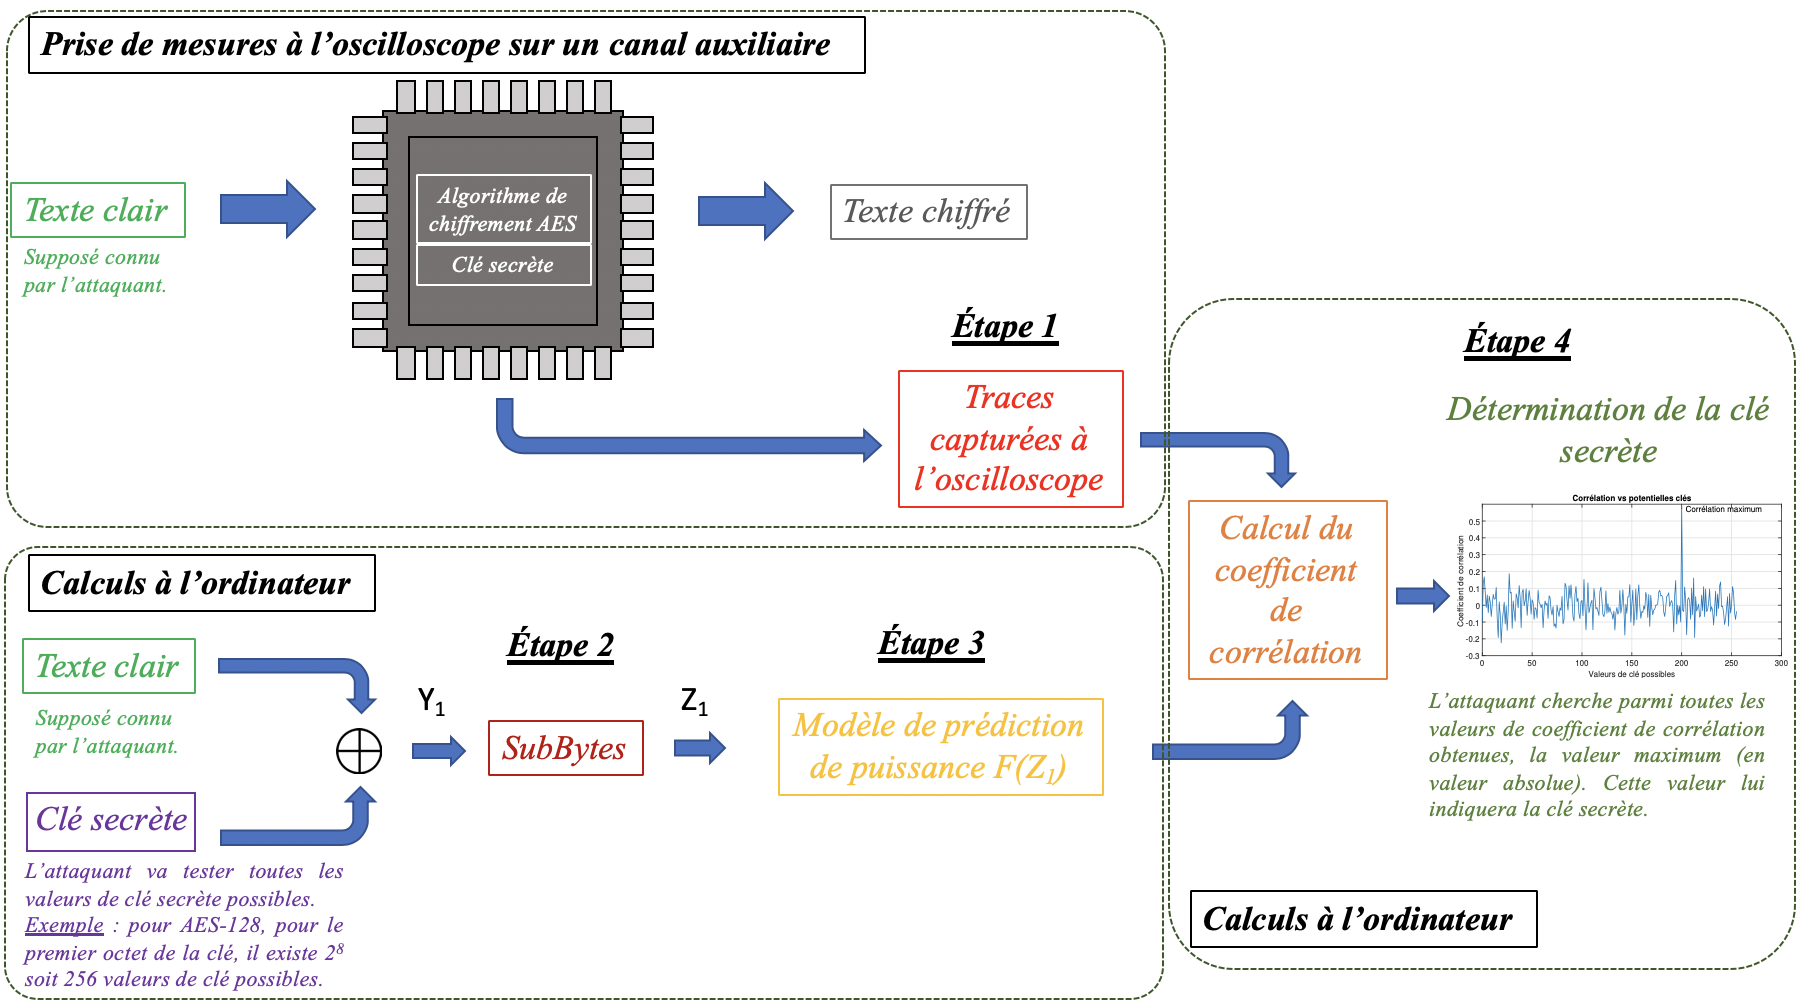
\includegraphics[scale=0.60]{image/CPA_attacks}
    \caption{Principe de fonctionnement d'une attaque CPA.}
    \label{fig:CPA_attacks}
\end{figure}

 \vspace{1cm}\hspace{-0.5 cm}Les figures \ref{fig:4KeysEx} et \ref{fig:TrueKey} présentent de manière générale l'évolution du coefficient de corrélation pour le huitième byte d'une clé de chiffrement. En effet, dans cet exemple, nous considérons que l'attaquant a pour tâche de retrouver le huitième byte d'une clé utilisée par l'AES-256 (pour rappel, une clé utilisée avec l'AES-256 possède une taille totale de trente-deux bytes). La première figure (\ref{fig:4KeysEx}) représente l'évolution du coefficient de corrélation au cours du temps pour quatre valeurs de clés différentes. On remarque un pic de corrélation plus élevé dans le graphe dédié à la clé 40. Il s'agit en effet de la vraie valeur du huitième byte de la clé employée par l'algorithme AES pour cet exemple. Pour encore mieux comprendre le principe de corrélation, la figure \ref{fig:TrueKey} présente la corrélation obtenue en fonction des 256 valeurs de clés testées (toujours pour le huitième byte de la clé). Sur ce graphe encore, on constate qu'il y a un pic de corrélation. Cette valeur maximale du coefficient de corrélation correspond à la clé 40. Ainsi, si l'attaquant souhaite retrouver les trente-deux bytes de la clé employée pour le chiffrement, il lui suffit de retrouver les trente-deux valeurs de clé correspondantes aux trente-deux valeurs maximales du coefficient de corrélation. Les deux figures (\ref{fig:4KeysEx} et \ref{fig:TrueKey}) sont présentées à la page suivante.

 \begin{figure}[htbp]
    \hspace{-2cm}
    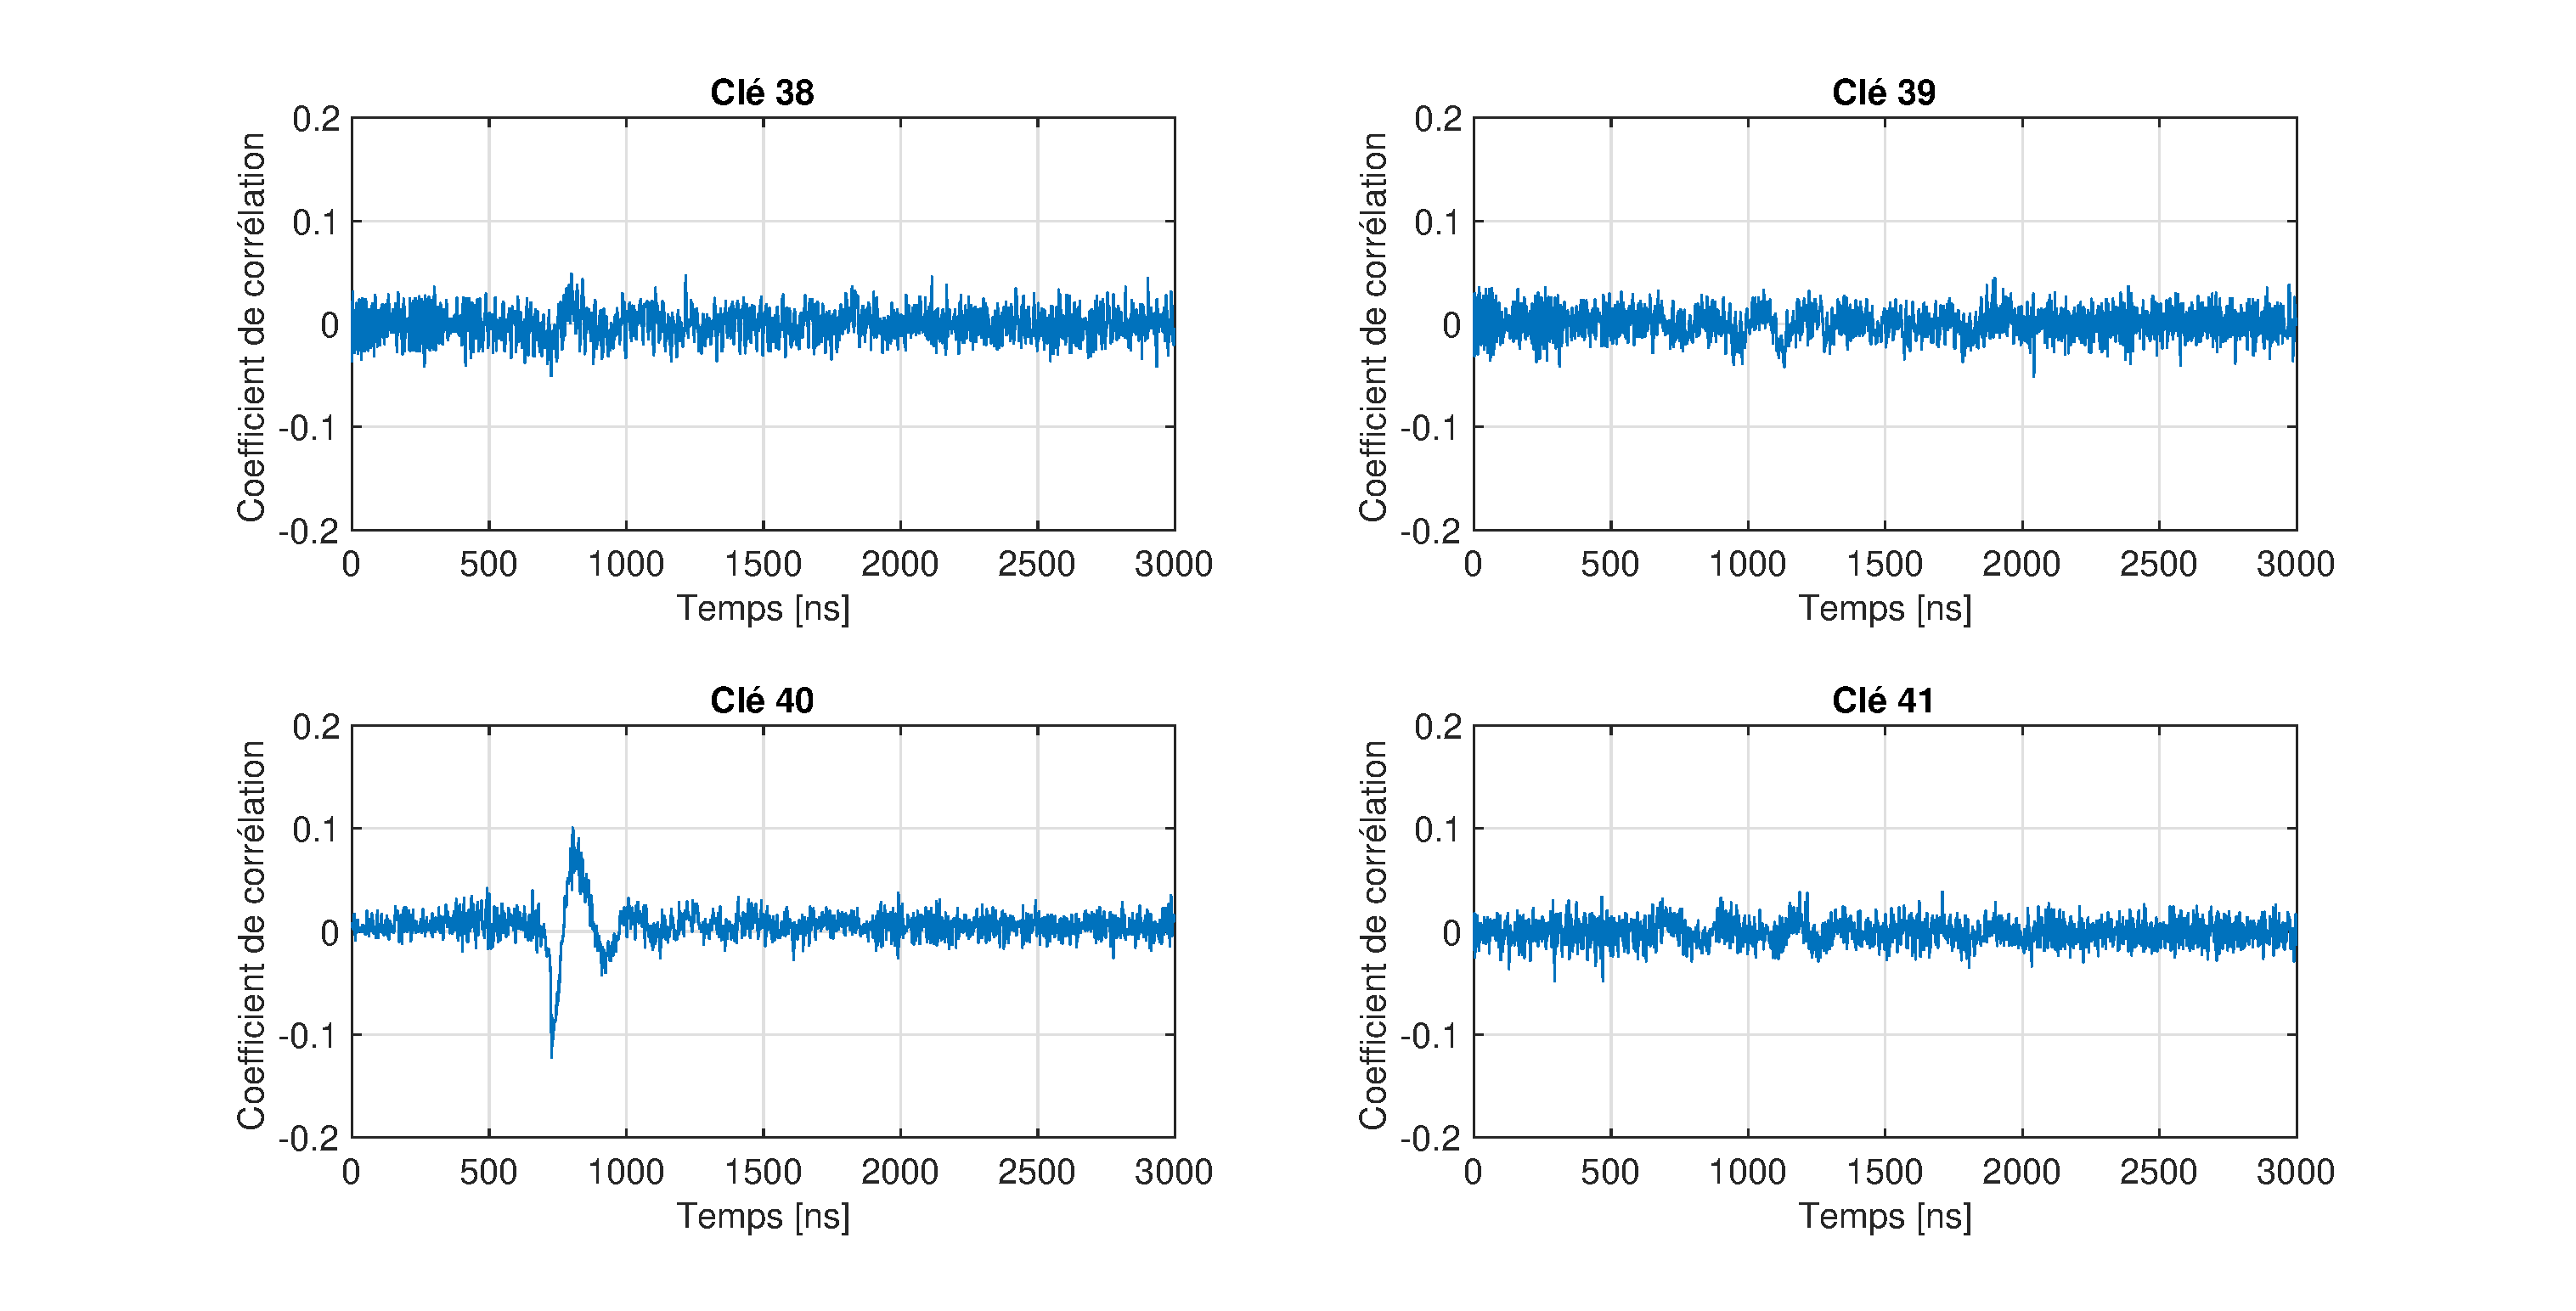
\includegraphics[scale=0.4]{image/4KeysEx}
    \caption{Différents résultats de corrélation en fonction de 4 clés testées.}
    \label{fig:4KeysEx}
\end{figure}

\begin{figure}[htbp]
    \hspace{-2cm}
    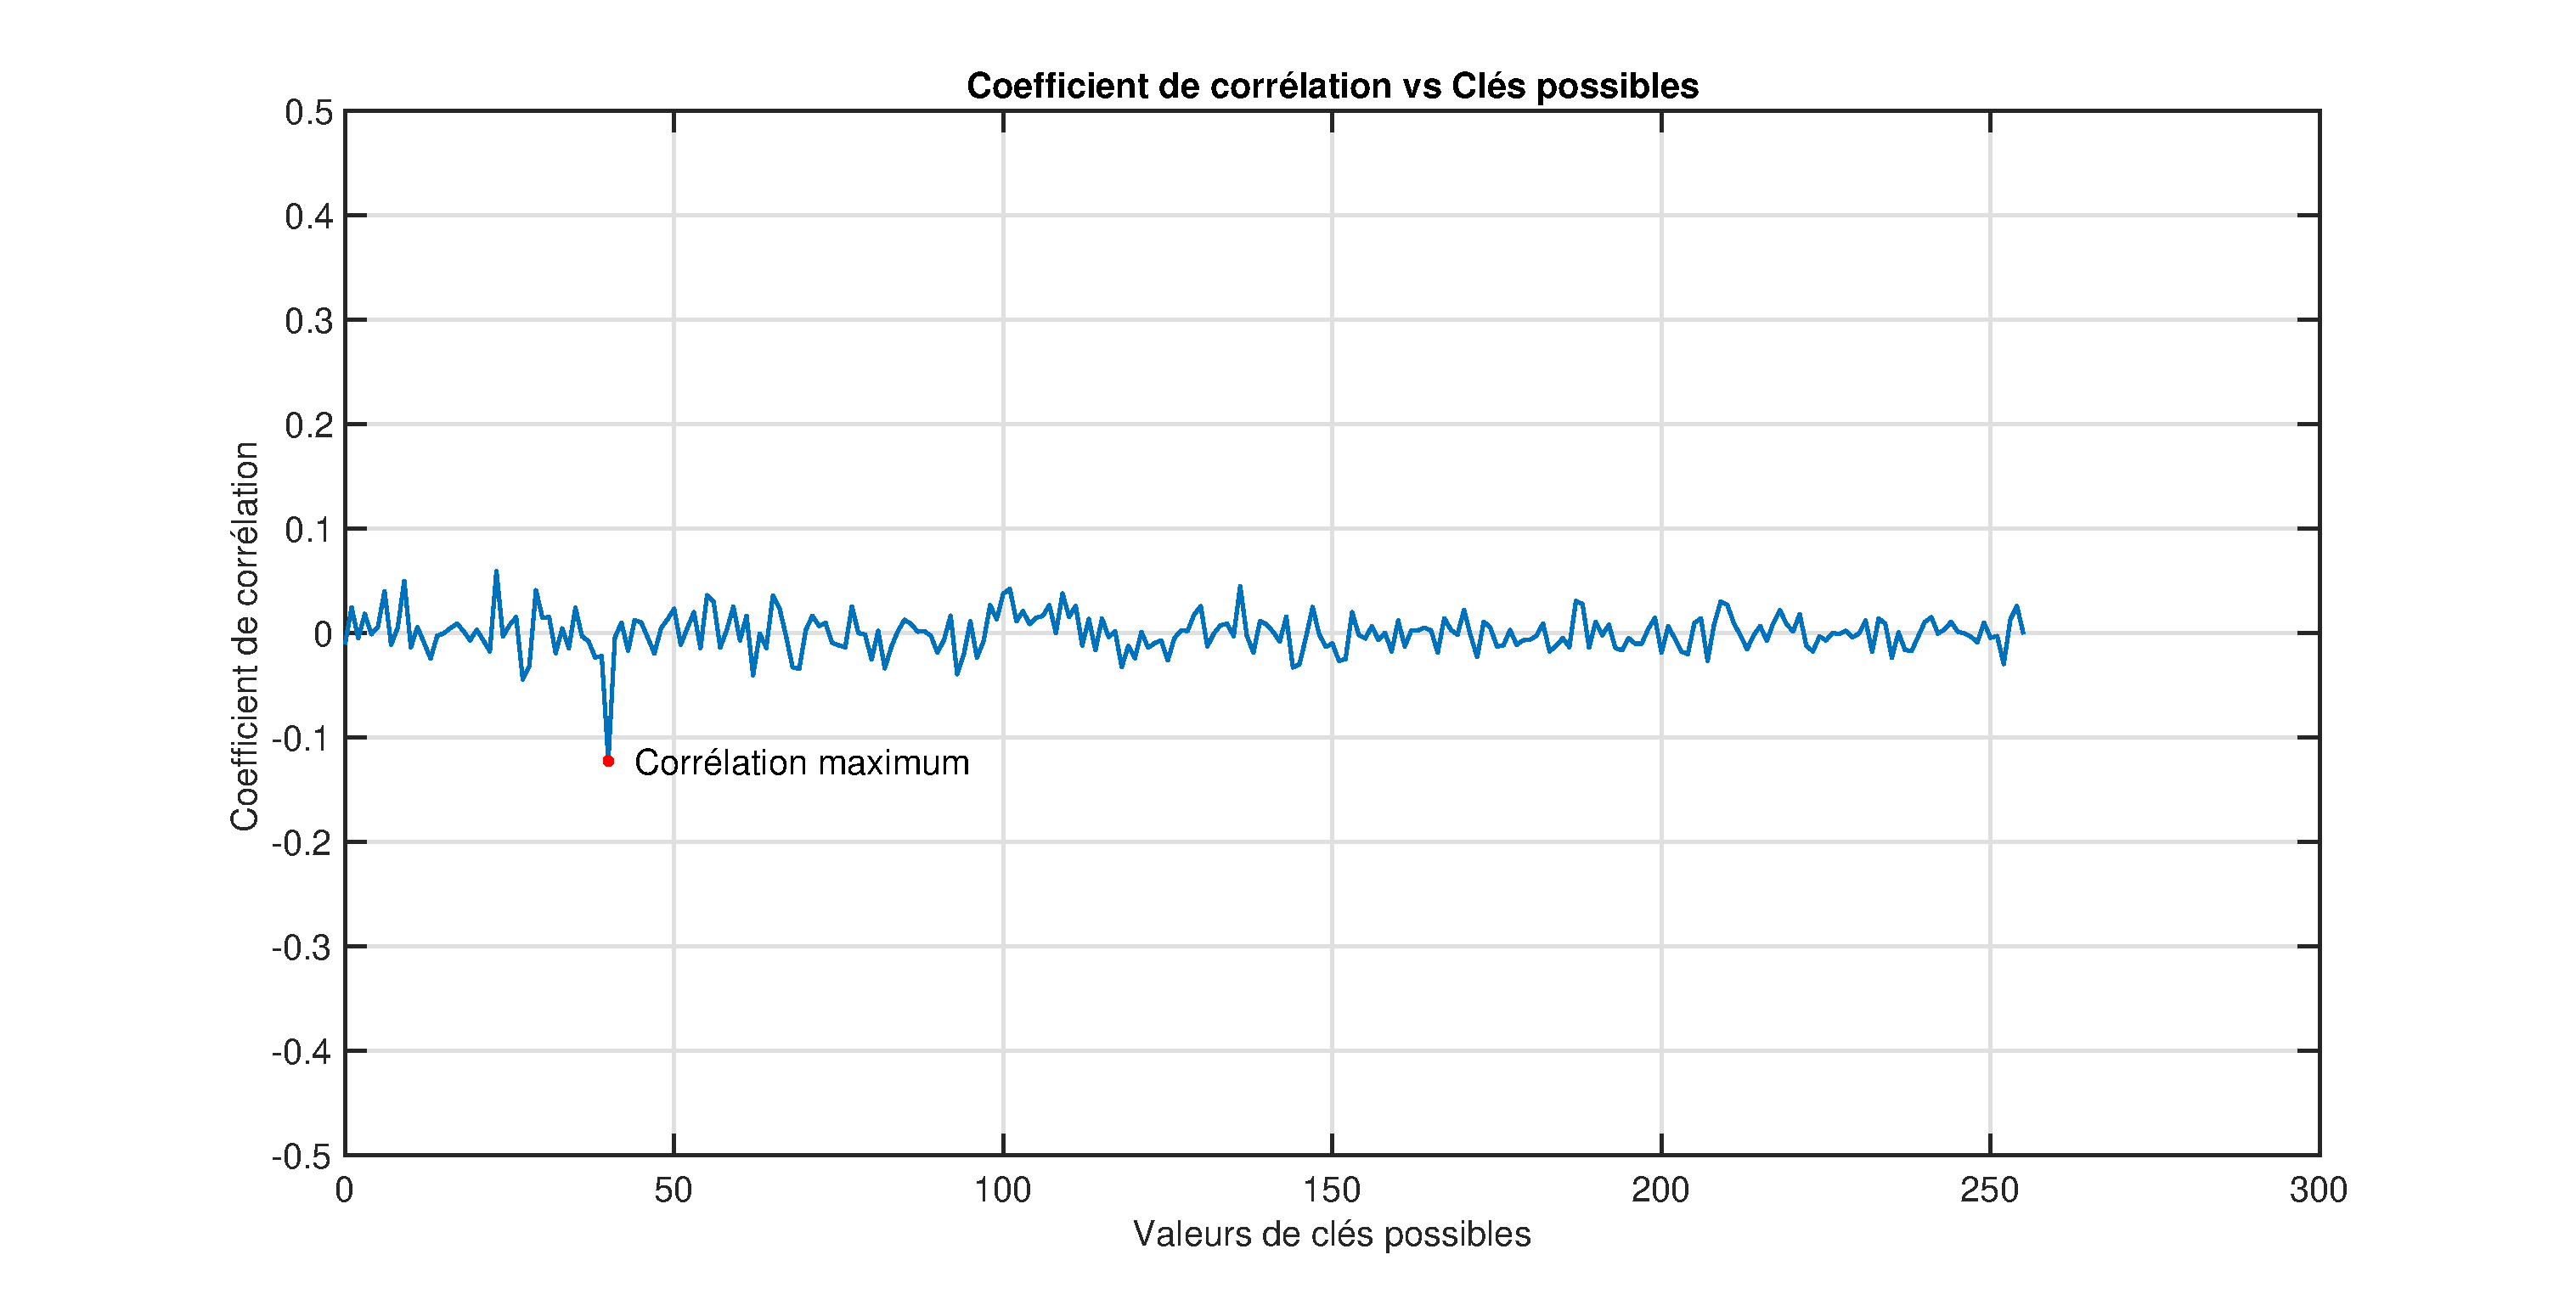
\includegraphics[scale=0.4]{image/TrueKey}
    \caption{Corrélation en fonction des 256 clés testées.}
    \label{fig:TrueKey}
\end{figure}




\newpage

%%%%%%%%%%%%% Chapitre 5 %%%%%%%%%%%%%

\chapter{Contre-mesures}
\label{chap:contremesure}

Ce cinquième et dernier chapitre de la partie \textit{théorie} introduit au lecteur les différents types de contre-mesures existantes permettant de neutraliser les attaques par analyse de la consommation de puissance. Tout d'abord, une introduction servant de préliminaires est présentée au lecteur. Ensuite, deux grands types de contre-mesures sont détaillés. Il s'agit des contre-mesures de type \textit{masking} et de type \textit{hiding}. Enfin, une contre-mesure particulière est définie. Il s'agit de la contre-mesure de type \textit{faking}, développée pour la réalisation de ce travail.

\section{Introduction}
\label{sec:intro_contremesure}

Dès que les attaques par analyse de la consommation de puissance ont été reconnues fonctionnelles, une série de contre-mesures fut développée afin d'empêcher la réussite de celles-ci. Les attaques CPA, au même titre que toute autre attaque utilisant l'analyse de la consommation de puissance (attaque SPA, attaque DPA, etc.), fonctionnent du fait que la consommation de puissance du device cryptographique dépend des valeurs intermédiaires exécutées par l'algorithme de chiffrement. Ainsi, l'objectif d'une contre-mesure est de casser cette relation qu'il existe entre la consommation de puissance et les données sensibles manipulées et entre la consommation de puissance et les opérations exécutées. On distingue deux grandes catégories de contre-mesures : 
\begin{enumerate}
\item \textbf{Les contre-mesures de type \textit{Hiding}} : Le principe des contre-mesures de type Hiding est de rendre la consommation de puissance du device cryptographique indépendante des opérations exécutées et des données manipulées. Pour ce faire, il existe deux approches différentes possibles. Ces deux approches sont détaillées à la section \ref{sec:hiding}.
\item \textbf{Les contre-mesures de type \textit{Masking}} : Le principe des contre-mesures de type Masking est de générer des valeurs intermédiaires aléatoires. Ainsi, on accepte que la consommation de puissance du device cryptographique dépende des données manipulées. Cependant, on modifie (on masque) volontairement ces valeurs intermédiaires afin de fausser les traces de puissance obtenues à l'oscilloscope. \\
\end{enumerate}

\hspace{-0.5cm}Il est donc important de bien comprendre que les contre-mesures développées pour les attaques par analyse de la consommation de puissance ont pour objectif général de modifier l'allure des traces de puissances afin de compliquer la tâche de l'attaquant. Il existe deux façons de modifier une trace de puissance : 
\begin{itemize}
\item En agissant sur \textbf{\textit{l'amplitude}} de la trace, on parlera \textbf{\textit{d'intensité du leakage.}}
\item En agissant sur \textbf{\textit{la position dans le temps}} de la trace, on parlera \textbf{\textit{d'instant du leakage.}} \\
\end{itemize}

\newpage

Les figures \ref{fig:trace_Amplitude} et \ref{fig:trace_Time} respectivement montrent comme modifier des traces de puissances en agissant d'une part sur l'amplitude (figure \ref{fig:trace_Amplitude}) et d'autre part sur la position dans le temps (\ref{fig:trace_Time}). Pour ces deux figures, nous affichons la consommation de puissance d'un FPGA en cours de chiffrement sur lequel est implémenté l'algorithme AES-256. Concernant la figure \ref{fig:trace_Amplitude}, le graphe de gauche affiche la consommation normale tandis que le graphe de droite affiche la consommation modifiée en amplitude. En effet, nous avons fait en sorte que la consommation de puissance soit plus uniforme en amplitude. Nous sommes passés d'une consommation qui variait entre [$\SI{-18.1}{\volt} ; \SI{9.7}{\volt} $] à une consommation qui varie entre [$\SI{-13.1}{\volt} ; \SI{4.9}{\volt} $]. Concernant la figure \ref{fig:trace_Time}, nous avons inversé l'ordre d'exécution des opérations. Dans cet exemple, nous avons imaginés deux opérations (ce n'est pas le cas en réalité), représentées par les cercles rouge et vert. Le graphe de gauche affiche la consommation normale tandis que le graphe de droite affiche la consommation \textit{retournée} dans le temps. En effet, certaines opérations sont parfois mélangées dans un algorithme cryptographique afin de nuire à l'attaque. Pour conclure, on se rend bien compte que la modification de ces traces de puissance, que ce soit en amplitude ou dans le temps, complexifie la tâche de l'attaquant étant donné qu'il ne possède plus les mêmes repères.
\begin{figure}[htbp]
    \centering
    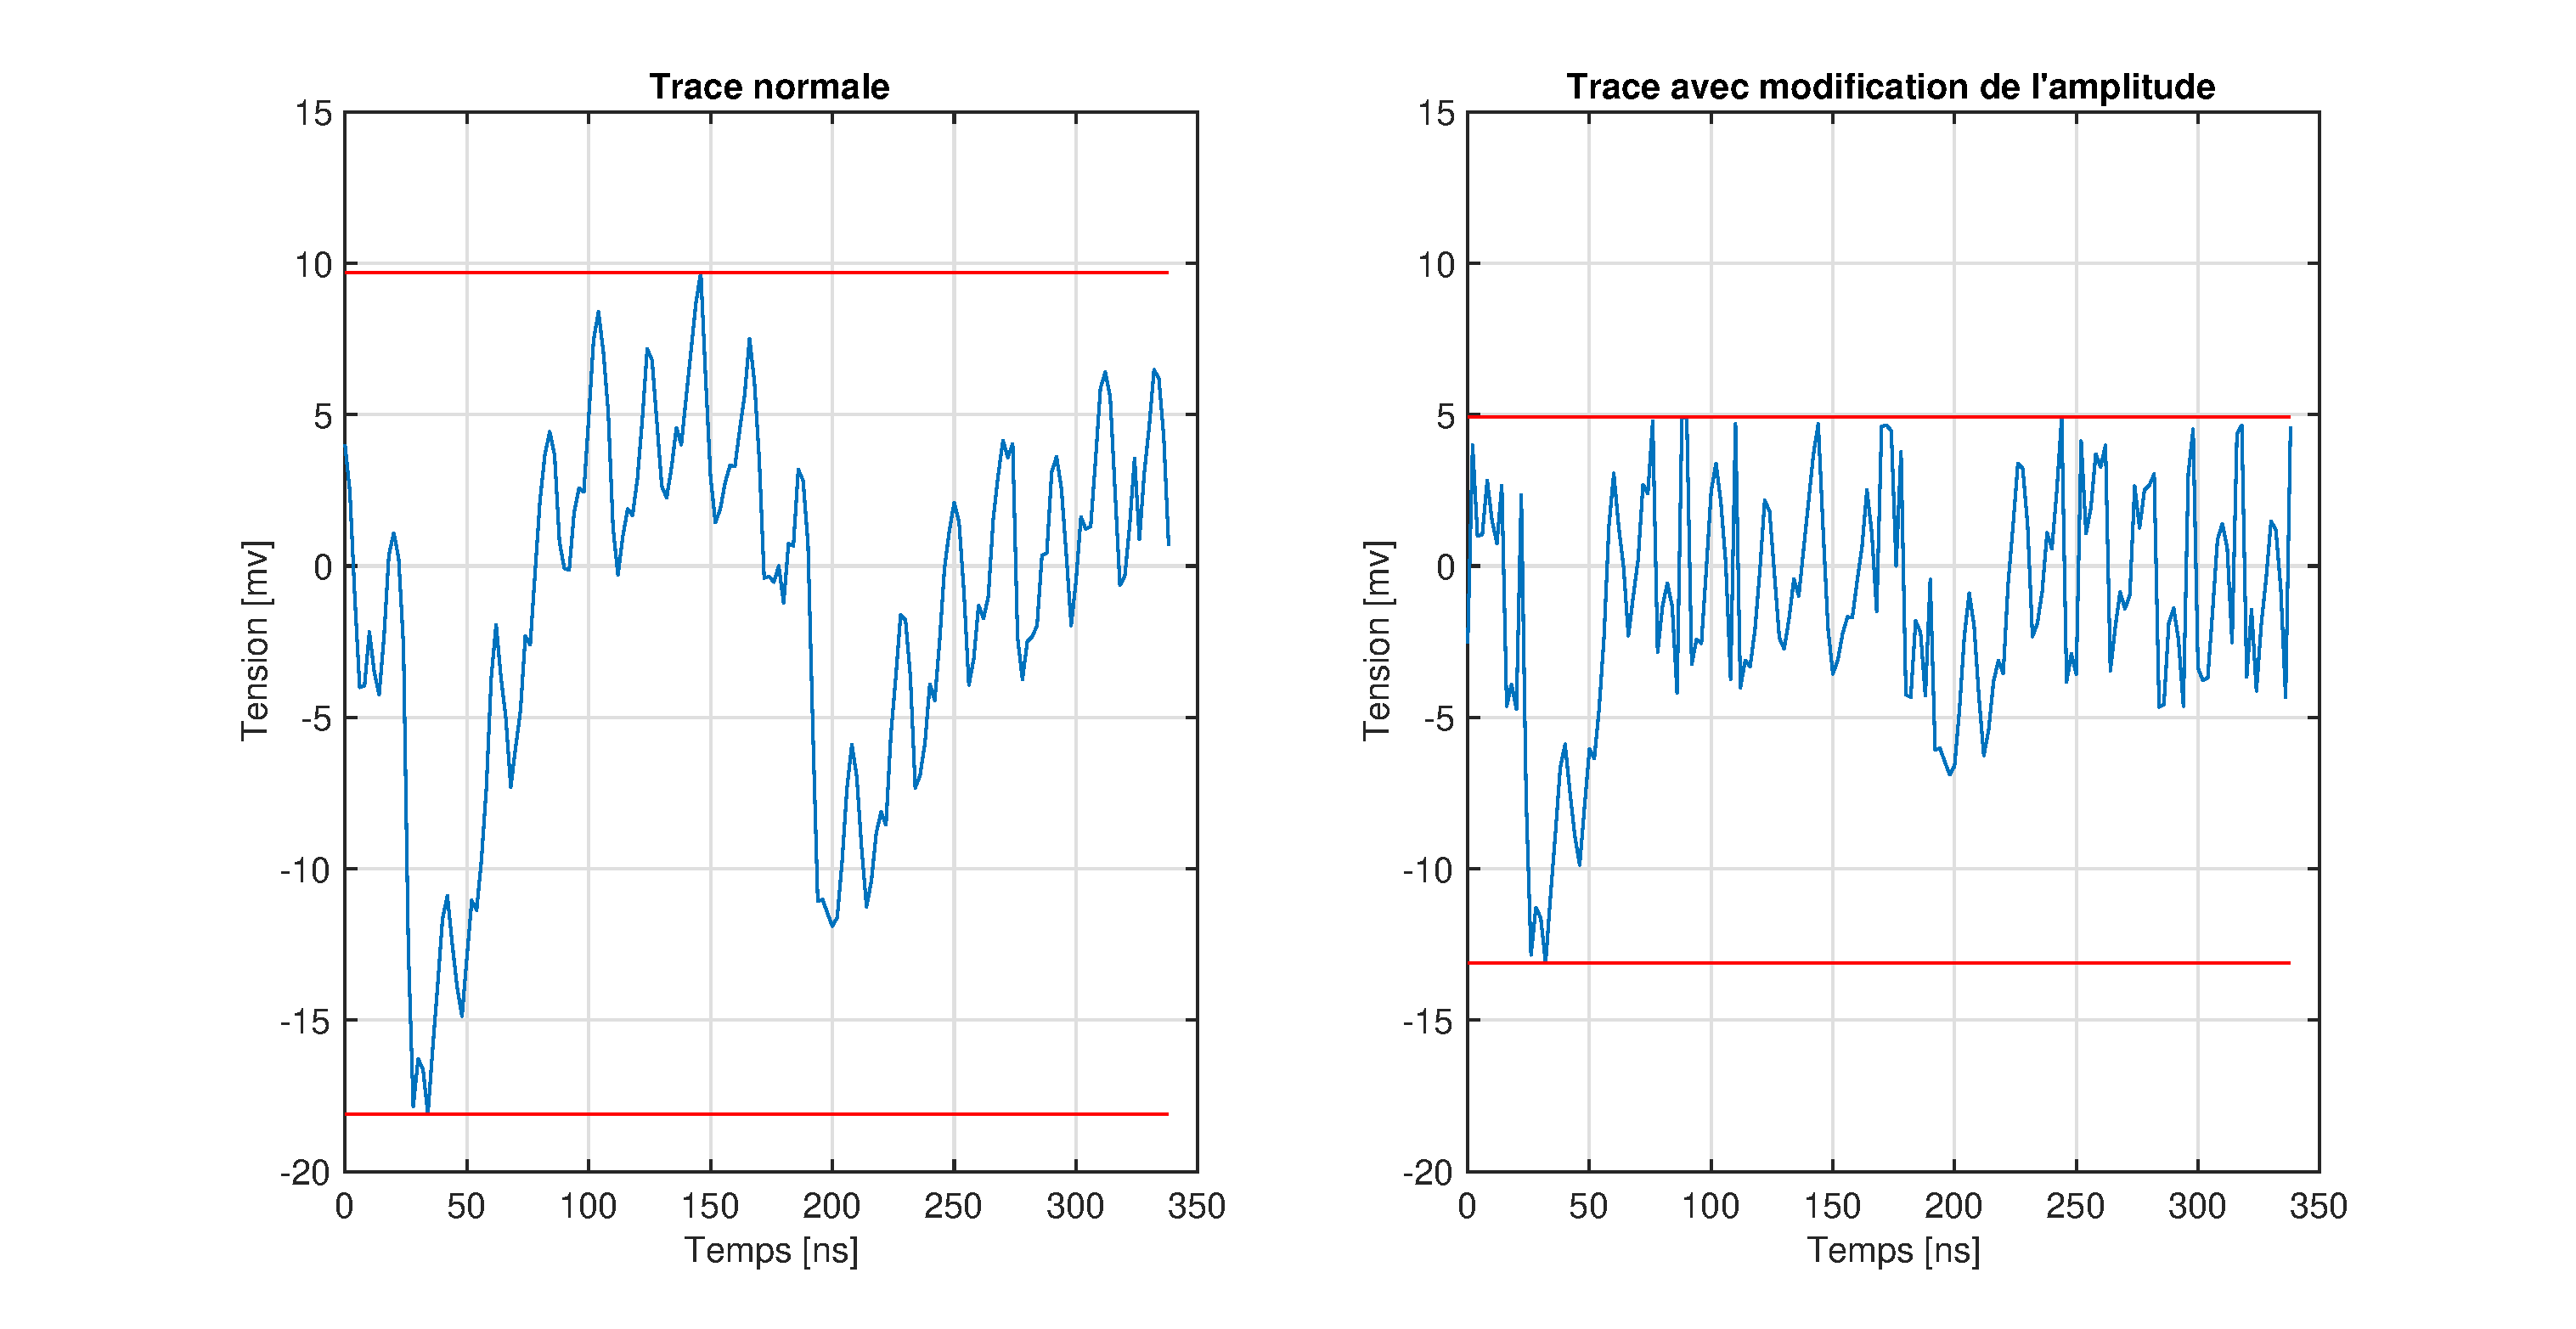
\includegraphics[scale=0.3]{image/trace_Amplitude}
    \caption{Modification de l'amplitude d'une trace de puissance.}
    \label{fig:trace_Amplitude}
\end{figure}

\begin{figure}[htbp]
    \centering
    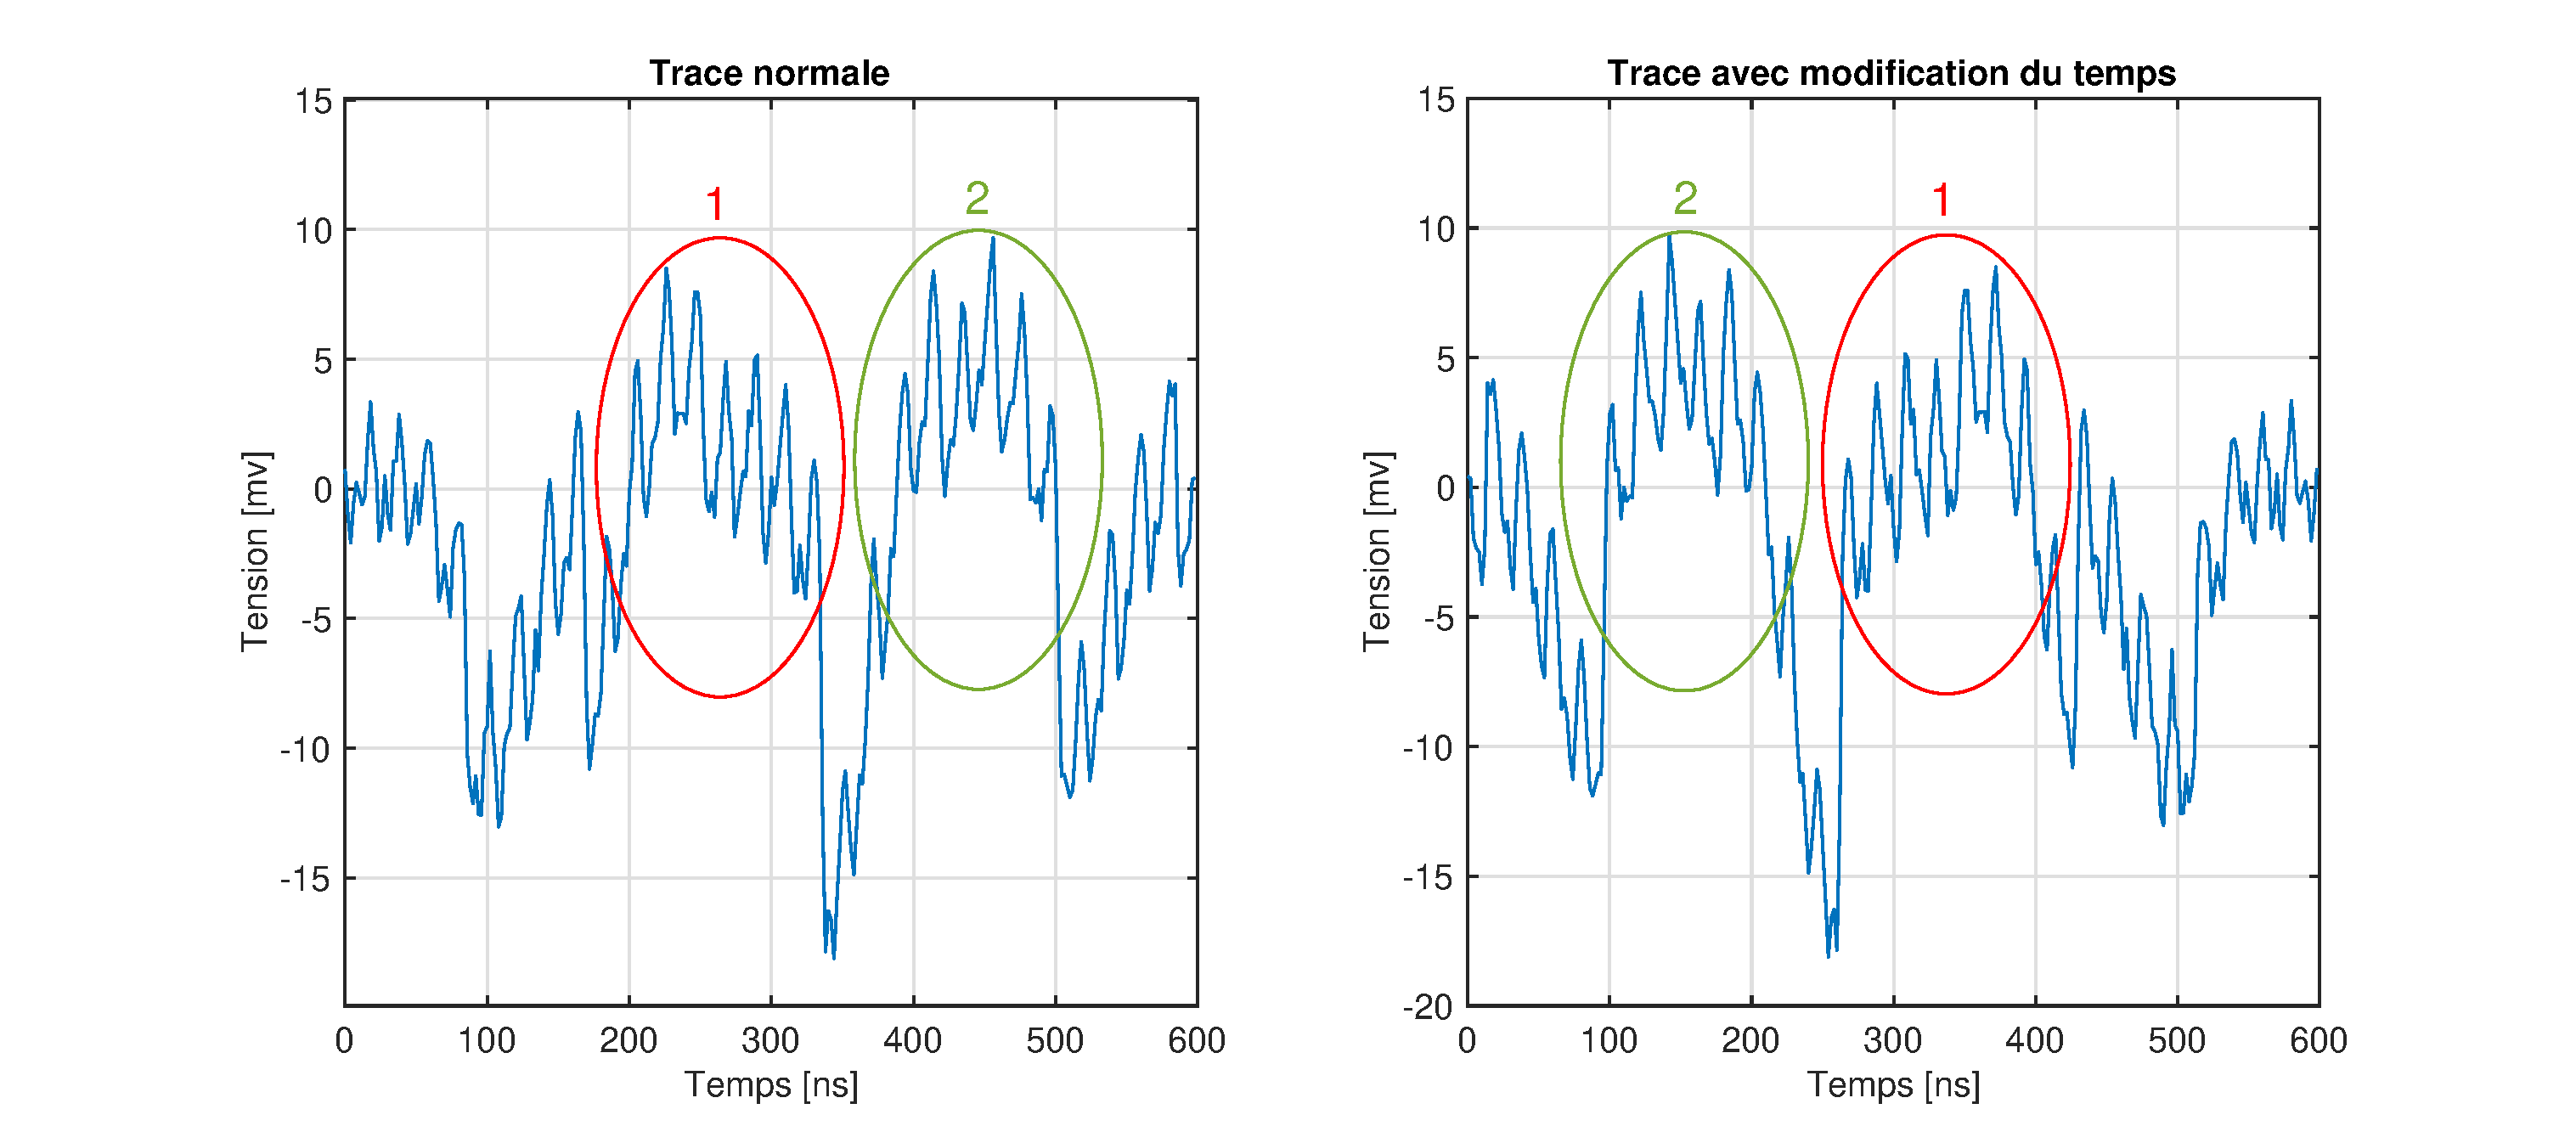
\includegraphics[scale=0.32]{image/trace_Time}
    \caption{Modification de la position dans le temps d'une trace de puissance.}
    \label{fig:trace_Time}
\end{figure}

\hspace{-0.5cm}Avant de détailler chacune des deux catégories de contre-mesures, rappelons la définition de rapport signal à bruit (SNR : \textit{Signal to Noise Ratio} en anglais). Sa définition est reprise ci-dessous. 

\theoremstyle{definition}
\begin{definition}{\textbf{Rapport Signal à Bruit (SNR) :}}
Le rapport signal à bruit ou SNR est un indicateur de performance. Son objectif est de mesurer la qualité de la transmission d'une information. Sa formulation mathématique est reprise à l'équation (\ref{eqn:SNR}). Elle peut également être exprimée en \textit{dB} (\ref{eqn:SNRdb}) : \\

\begin{gather}
	SNR = \frac{P_{signal}}{P_{noise}} \label{eqn:SNR}
\end{gather}
\begin{gather}
	SNR_{dB} = 10.log_{10}\frac{P_{signal}}{P_{noise}} \label{eqn:SNRdb}
\end{gather}

\hspace{-0.5 cm}Où :
\begin{itemize}
\item $SNR$ ($SNR_{dB}$) représente l'indicateur de performance de la transmission de l'information sans unité (en dB).
\item $P_{signal}$ représente la puissance du signal (en \textit{Watt}).
\item $P_{noise}$ représente la puissance du bruit (en \textit{Watt}). \\
\end{itemize}
\end{definition}

\vspace{-0.4 cm}\hspace{-0.5 cm}Ainsi, le calcul du SNR permet d'évaluer si le signal de transmission que l'on étudie est fortement bruité ou non. Selon l'équation (\ref{eqn:SNR}), cet indicateur SNR est d'autant plus élevé que la puissance du signal est élevée ou est d'autant plus élevé que la puissance du bruit est faible. Dans une transmission idéale, on désirera toujours un SNR très grand, signifiant que la trace obtenue représente majoritairement le signal et minoritairment le bruit (qui pour rappel est un élément parasite aléatoire).

\hspace{-0.5 cm}Pour une trace de puissance, si le SNR d'une opération est élevé, cela signifie que la puissance du signal est plus élevée que la puissance du bruit, c'est-à-dire qu'il est plus facile de détecter des fuites d'information. Idéalement, il faut donc que le SNR soit proche de 0. De cette façon, le bruit recouvre tellement le signal qu'il est impossible pour l'attaquant de détecter du \textit{leakage} (fuite d'information). En pratique, cela peut être réalisé en diminuant la variance du signal vers 0 ou en augmentant la variance du bruit vers l'infini.
\begin{itemize}
\item Pour réduire la variance du signal, la consommation de puissance a besoin d'être exactement égale pour toutes les opérations exécutées et données manipulées. En pratique, cela se traduira par de petites valeurs de variances pour le signal.
\item Pour augmenter la variance du bruit, l'amplitude du bruit a besoin d'être augmentée de façon significative laissant croire à l'attaquant l'existence de commutations sur les cellules du device. En pratique, cela se traduira par de grandes valeurs de variances pour le bruit.
\end{itemize}

\hspace{-0.5 cm}La figure \ref{fig:SNR_Fig} ci-dessous présente une fonction sinusoïdale sans bruit (gauche) et avec bruit (droite). 
\begin{figure}[htbp]
    \centering
    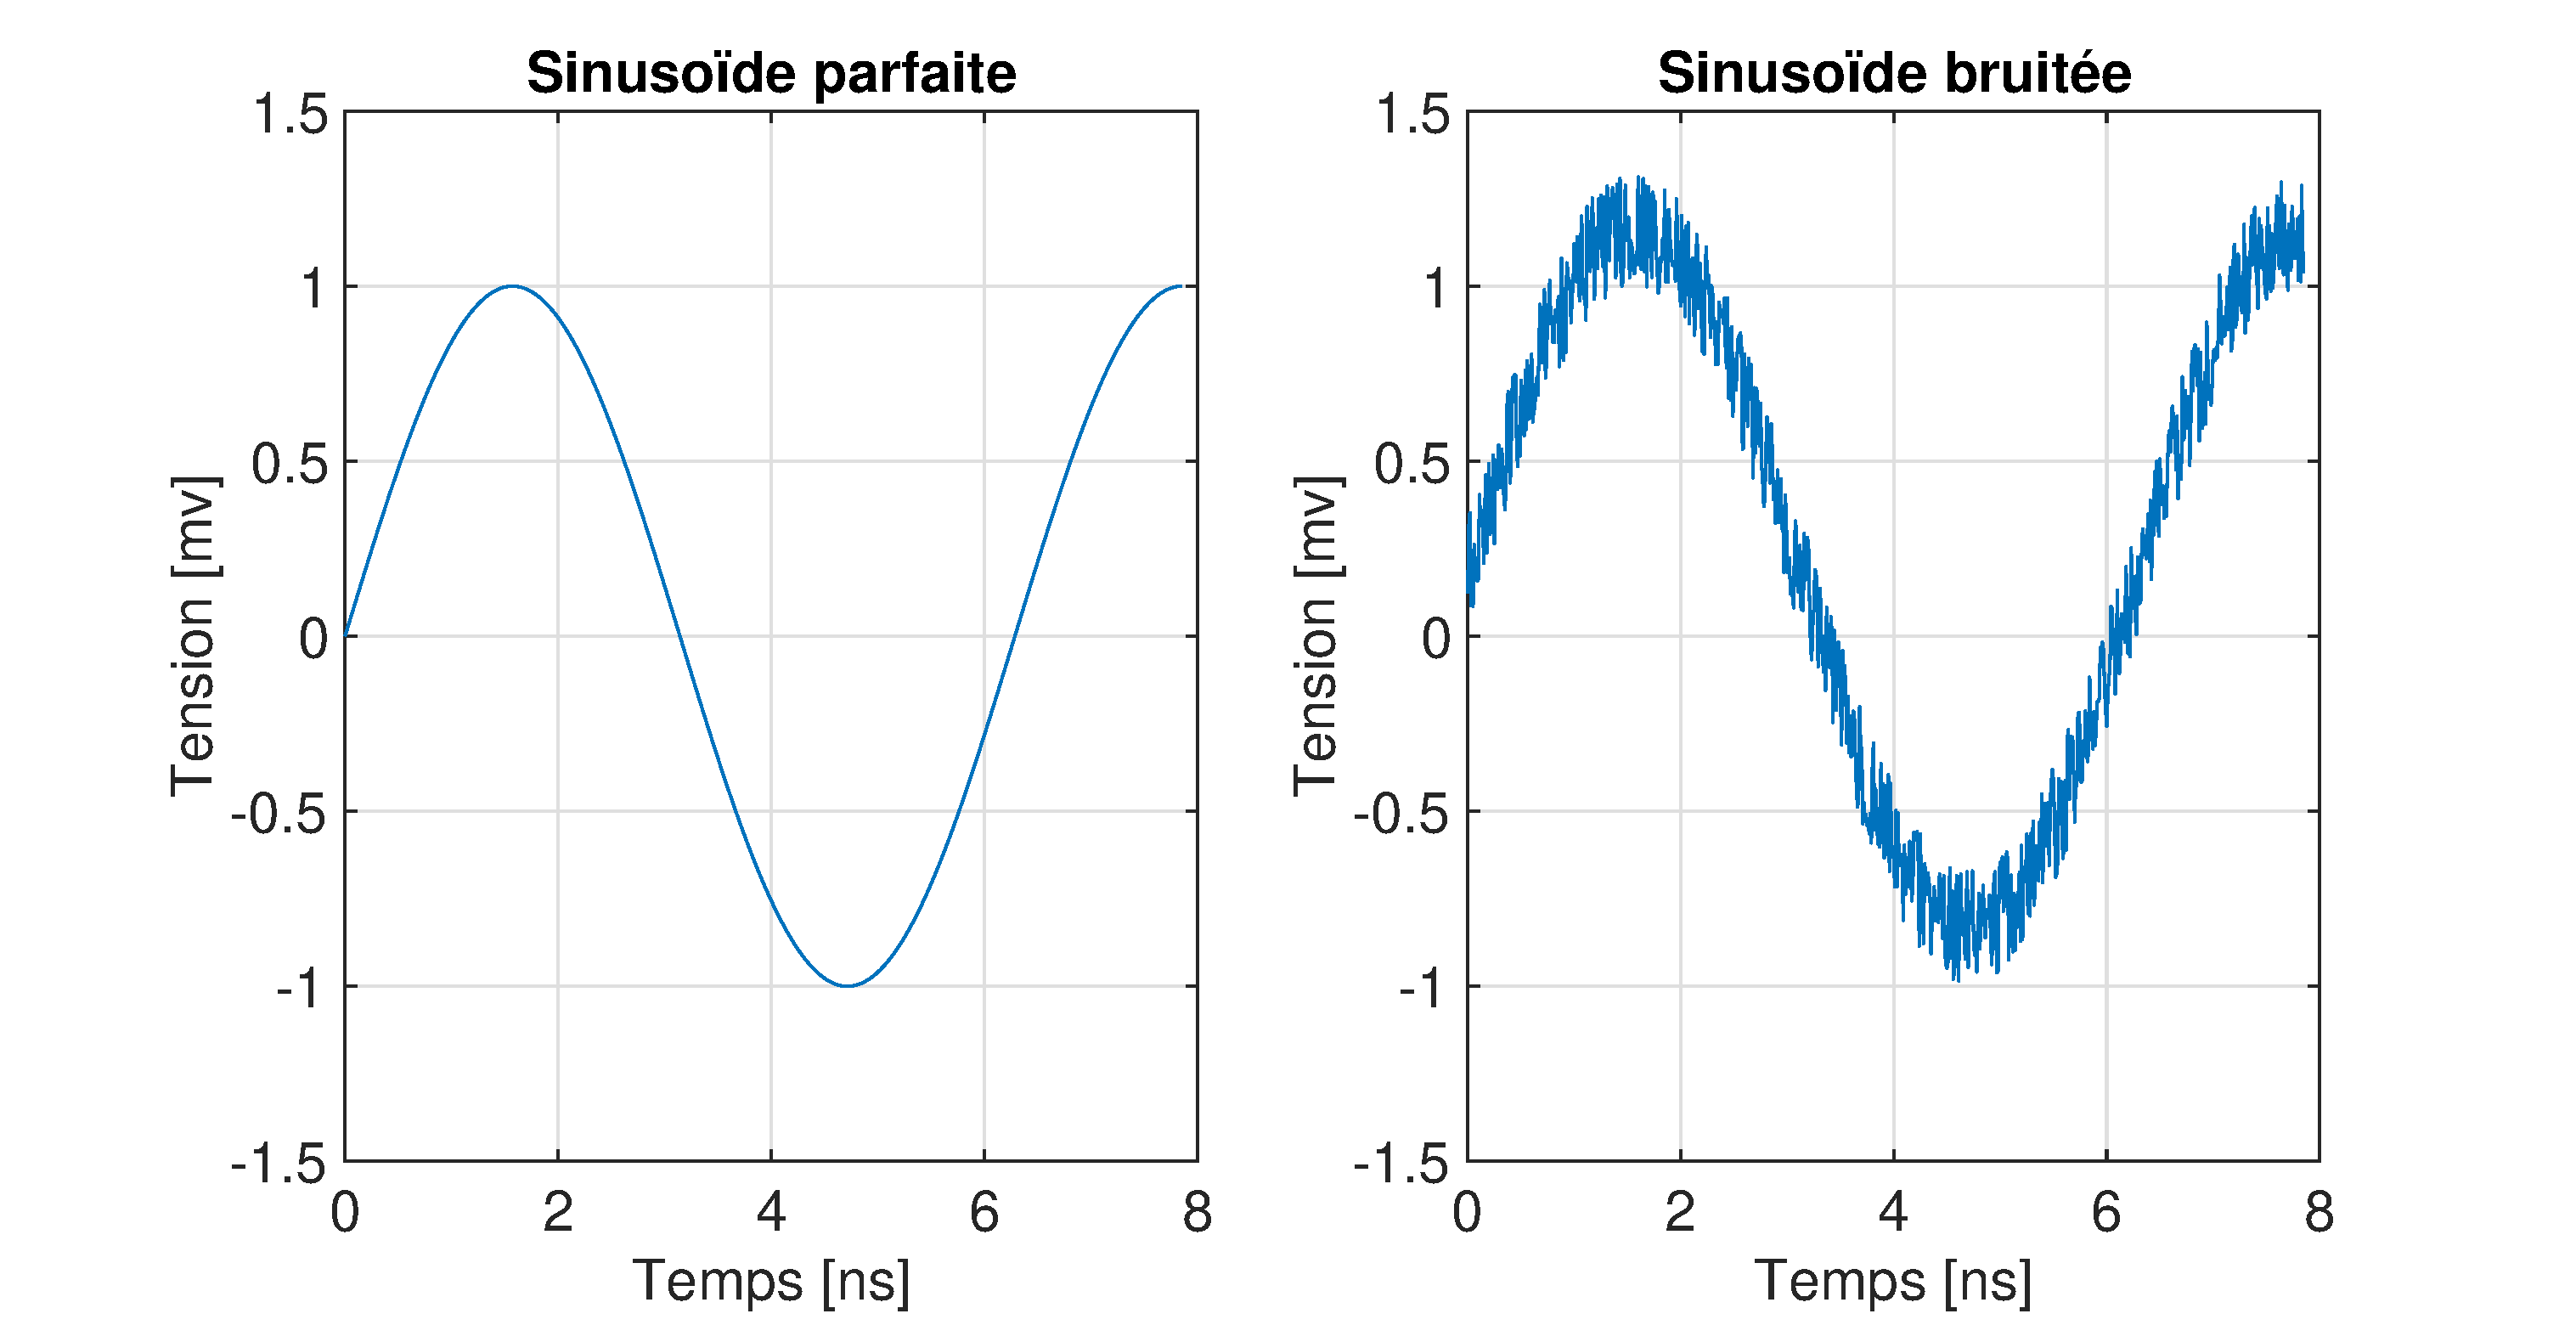
\includegraphics[scale=0.2]{image/SNR_Fig}
    \caption{Importance du bruit pour un signal de transmission.}
    \label{fig:SNR_Fig}
\end{figure}

\newpage

\section{Contre-mesures Hiding}
\label{sec:hiding}

\vspace{-0.1 cm}Comme précisé ci-avant, le principe des contre-mesures de type Hiding est de rendre la consommation de puissance du device cryptographique indépendante des opérations exécutées et des données manipulées. Pour ce faire, deux approches sont possibles :
\begin{enumerate}
\item Faire en sorte que la consommation de puissance du device cryptographique soit \textbf{\textit{aléatoire}}. Cela signifie qu'à chaque coup de clock, une certaine quantité aléatoire de puissance est consommée. Le but est donc de \textbf{modifier l'instant du leakage} ou bien de \textbf{modifier l'intensité du leakage} dans la trace de puissance.
\begin{itemize}
\item \textit{La modification de l'instant du leakage peut être réalisée par un désalignement des traces}. Cela va compliquer la tâche de l'attaquant. En effet, celui-ci doit, dans un premier temps, procéder à l'alignement de ses traces pour pouvoir les analyser correctement. Si celles-ci ne sont pas alignées, il ne pourra rien en tirer de concret. Ce désalignement des traces peut s’obtenir de différentes façons : utiliser des horloges de fréquences différentes, utiliser des interruptions aléatoires lors de l’exécution du programme, changer l’ordre des instructions, etc.
\item \textit{La modification de l'intensité du leakage peut être réalisée par une modification du rapport signal à bruit}. Nous avons vu que pour diminuer le SNR, il suffisait d'augmenter le bruit ou de diminuer le signal. Dans ce cas-ci, nous allons augmenter la variance du bruit. En effet, en ajoutant du bruit de façon indépendante à l'exécution de l'algorithme, on va diminuer le SNR, ce qui va avoir pour conséquence de diminuer le leakage d'une opération : L'attaquant aura dès lors plus de difficultés à retrouver la clé secrète. On peut, pour ce faire, utiliser un filtre afin de ne laisser passer que certaines composantes de puissance ou encore utiliser ce qu'on appelle des "\textit{noise engines}", systèmes fonctionnant en parallèle du device cryptographique et ayant pour but de générer du bruit.
\end{itemize}
\item Faire en sorte que la consommation de puissance du device cryptographique soit \textbf{\textit{identique}}. Cela signifie qu'à chaque coup de clock, une quantité égale de puissance est consommée pour toutes les opérations exécutées et pour toutes les données manipulées. Le but est donc de \textbf{modifier l'intensité du leakage}. Autrement dit, on souhaite uniformiser l'amplitude de la trace. 
\textit{Pour ce faire, on va à nouveau modifier le rapport signal à bruit}. L'idéal étant d'avoir un SNR proche de 0, si on n'augmente pas la variance du bruit, la deuxième approche consiste à diminuer la variance du signal. Pour ce faire, on va modifier de façon physique les cellules CMOS. En effet, le but est de faire en sorte que chaque cellule logique consomme la même consommation de puissance pour toute opération demandée. \\
\end{enumerate}

\hspace{-0.5cm}Le tableau \ref{tab:hiding} ci-dessous présente les paramètres influencés pour la réalisation d'une contre-mesure selon le type d'approche suivi (puissance équivalente ou aléatoire) tandis que l'annexe \ref{ann:resume_hiding} reprend un ensemble de contre-mesures de type hiding. Pour rappel, des exemples de modification de l'intensité du leakage et de l'instant du leakage pour une trace de puissance ont été donnés en introduction de ce chapitre (voir figures \ref{fig:trace_Amplitude} et \ref{fig:trace_Time}).

\begin{table}[htbp]
	\centering
	\begin{tabular}{|c|c|}
    		\hline
   		  \textit{Consommation de puissance \textbf{équivalente}} & \textit{Consommation de puissance \textbf{aléatoire}} \\ \hline 
   		  \textbf{Intensité} du leakage &  \textbf{Instant} du leakage \\ 
   		   &  \textbf{Intensité} du leakage \\ \hline
	\end{tabular}
    	\caption{Les contre-mesures de type hiding sont utilisées pour rendre aléatoire ou égale la consommation de puissance du device cryptographique..}
    	\label{tab:hiding} 
\end{table}

\hspace{-0.5 cm}Sur base de l'annexe \ref{ann:resume_hiding}, nous pouvons expliquer le principe de fonctionnement de certains exemples de contre-mesures :
\begin{itemize}
\item Concernant la manipulation d’horloge, nous pouvons :
\begin{itemize}
\item Ignorer certains coups de clock : ce qui aura pour effet de retarder l’exécution du prochain cycle, ce qui engendrera donc un désalignement des traces.
\item Changer aléatoirement la fréquence de clock : à l’aide d’un oscillateur et de nombres aléatoires, la fréquence d’horloge est changée à intervalles fréquents, provoquant des vitesses d’exécution différentes et par conséquent un désalignement des traces.
\end{itemize}
\item Concernant les interruptions : on va générer aléatoirement certaines interruptions lors de l'exécution de l'algorithme, ce qui va \textit{casser} (couper) les traces provoquant ainsi un désalignement.
\item Concernant la manipulation d'instructions : 
\begin{itemize}
\item Le mélange des instructions : on va mélanger l’ordre des opérations (seules les opérations qui peuvent être déplacées ou interverties). Ainsi, pour AES par exemple, il est possible de réaliser l’opération \textit{subBytes} sur les 16 bytes de la matrice, dans n’importe quel ordre, sans nuire au déroulement de l’algorithme.
\item Les instructions inutiles : en insérant des opérations inutiles, on va injecter des quantités d'informations inutiles dans chaque trace. Cela provoquera un désalignement des traces.
\item Le choix des instructions : toutes les instructions ne "fuitent" pas la même quantité d’information sur les opérandes. Il pourrait être bon de choisir les instructions qui révèlent le moins d’informations utiles à un attaquant ou de remplacer certaines instructions par d’autres instructions équivalentes pour que la fuite d’information ne soit pas toujours la même.
\end{itemize}
\item Concernant la diminution du SNR :
\begin{itemize}
\item On peut diminuer le SNR en augmentant la variance du bruit à l'aide de \textit{noise engines}. Il s'agit de composants hardware qui travaillent en parallèle à l’exécution cryptographique. Autrement dit, ces composants hardware vont générer du bruit, ce qui va avoir pour conséquence de diminuer le SNR. En effet, la consommation mesurée sera la somme de la consommation de l’exécution de l’algorithme cryptographique et des composants hardware.
\item On peut diminuer le SNR en diminuant la variance du signal. En pratique, il existe deux possibilités pour diminuer la variance du signal :
\begin{itemize}
\item Une première approche pourrait concerner la cellule logique CMOS en elle-même. On sait (section \ref{sec:puissance}) que la consommation de puissance totale d'un device cryptographique est la somme des puissances consommées par chaque cellule. Ainsi, si chaque cellule consomme une puissance constante, la puissance totale est constante. Il faut donc construire des cellules qui consomment des quantités de puissance constantes.
\item Une seconde approche plus complexe concerne le filtrage. Il s'agit de filtrer la puissance consommée par le device cryptographique. Le but est alors de supprimer, via ce filtre, toutes les composantes de la trace de puissance qui dépendent des données manipulées et des opérations exécutées. \\
\end{itemize}
\end{itemize}
\end{itemize}

En conclusion, le développement d'une contre-mesure de type hiding se concrétise soit en modifiant le \textit{design} du circuit électronique lors de sa conception (fabrication) soit en manipulant les coups de clocks et/ou les instructions devant être opérées par le circuit électronique. Par conséquent, ce type de contre-mesure prend du temps à être développé et est généralement assez compliqué à mettre en oeuvre.

\section{Contre-mesures Masking}
\label{sec:masking}

Le principe des contre-mesures de type masking est de générer des valeurs intermédiaires aléatoires. Autrement dit, lors de l'exécution d'un algorithme de chiffrement, différentes opérations sont exécutées conduisant à différentes valeurs intermédiaires calculées. Si aucune protection n'est mise en place, la consommation de puissance du device cryptographique dépendra des données intermédiaires qui sont manipulées par le device cryptographique (par l'algorithme précisément). L'attaquant peut alors potentiellement retrouver la clé secrète en enregistrant la consommation de puissance du device cryptographique et en réalisant une attaque de type CPA par exemple. Par contre, si chaque valeur intermédiaire est dissimulée sous une nouvelle valeur intermédiaire aléatoire dite \textbf{masquée}, alors l'attaquant pourra toujours analyser la consommation de puissance, les traces qu'il obtiendra fourniront des informations faussées (par le masque). En d'autres mots, ce type de contre-mesure accepte que la consommation de puissance du device cryptographique dépend des données manipulées et des opérations exécutées. Cependant, on va modifier les valeurs intermédiaires de façon aléatoire pour que les traces mesurées à l'oscilloscope n'aient plus de sens. Un avantage de cette approche est qu'elle peut être implémentée au niveau de l'algorithme, c'est-à-dire sans changer les caractéristiques de consommation de puissance du device cryptographique (ce qui est plus complexe) comme c'est le cas pour les contre-mesures de type \textit{Hiding}. La définition \ref{def:masque} ci-dessous permet de comprendre le principe de masquage. 

\theoremstyle{definition}
\begin{definition}{\textbf{Masque :}}
Une valeur intermédiaire masquée $v_m$ est une valeur intermédiaire $v$ cachée par une valeur aléatoire $m$. On obtient donc la relation suivante (\ref{eqn:masking}) : 
\begin{gather}
	v_m = v * m\label{eqn:masking}
\end{gather}
\end{definition}
\label{def:masque}

\hspace{-0.5cm}Ne connaissant pas la valeur aléatoire $m$, l'attaquant ne peut pas retrouver la valeur intermédiaire $v$. Ainsi, la consommation de puissance du device cryptographique dépend des valeurs intermédiaires masquées $v_m$ qui ne fournissent aucune information sur les valeurs intermédiaires $v$. Autrement dit, un masque cache les valeurs intermédiaires et il n'est donc plus possible de retrouver la clé de chiffrement. Bien évidemment, les masques ont besoin d'être supprimés à la fin des opérations algorithmiques afin d'obtenir \textit{in fine} le \textit{vrai} message chiffré. Autrement, le message chiffré obtenu serait également masqué et n'aurait donc aucun sens.

\hspace{-0.5cm}Le symbole $*$ dans (\ref{eqn:masking}) représente le type d'opérateur utilisé pour appliquer le masque sur les valeurs intermédiaires. Il peut s'agir d'une fonction booléenne ou d'une fonction arithmétique. Ainsi, on définit : 

\theoremstyle{definition}
\begin{definition}{\textbf{Masque booléen:}}
l'opération $*$ est remplacée par la fonction booléenne XOR (\oplus). Dans ce cas, le masque devient (\ref{eqn:maskingBool}):
\begin{gather}
	v_m = v \oplus m\label{eqn:maskingBool}
\end{gather}
\end{definition}
\theoremstyle{definition}
\begin{definition}{\textbf{Masque arithmétique:}}
l'opération $*$ est remplacée par une addition modulaire ($+$) ou par une multiplication modulaire (\times ). Dans ce cas, le masque devient (\ref{eqn:maskingArith1} ou \ref{eqn:maskingArith2}): 
\begin{gather}
	v_m = v + m \ (mod \ n)\label{eqn:maskingArith1}
\end{gather}
ou
\begin{gather}
	v_m = v \times m \ (mod \ n)\label{eqn:maskingArith2}
\end{gather}
où \textit{modulo n} est définit en fonction de l'algorithme de chiffrement.
\end{definition}

En conclusion, le développement d'une contre-mesure de type masking est plus facilement réalisable que le développement d'une contre-mesure de type hiding. En effet, ce type de contre-mesure consiste à s'intéresser à l'exécution des opérations d'un algorithme cryptographique (à ses valeurs intermédiaires) et d'ensuite modifier ces valeurs intermédiaires au travers de fonctions de masquage. Même si le principe semble facile en théorie, attention tout de même à la mise en application. En effet, certaines contre-mesures proposées sont considérablement compliquées à comprendre et à traduire en langage machine.

\section{Contre-mesures Faking}
\label{sec:faking}

Le choix de la contre-mesure à développer dans le cadre de mon travail ne m'ayant pas été imposé, après diverses recherches dans les livres de références et dans les articles sur \textit{Internet}, j'ai trouvé un nouveau principe de contre-mesure. Ce type de contre-mesure se dénomme \textbf{\textit{Faking}}. Cette contre-mesure s'appuie sur une partie du concept de contre-mesure par \textit{Masking} mais avec quelques subtilités. C'est donc ce type de contre-mesure que j'ai décidé de développer dans le cadre de mon travail. Les résultats seront présentés au chapitre \ref{chap:faking} (Partie 2).

\subsection{Définition}
\label{subsec:def}

\hspace{-0.5 cm}L'objectif de la contre-mesure est le suivant : Dès le départ, on va venir masquer la vraie valeur de clé ($Key_{Real}$) en opérant un XOR avec un masque ($Key_{Mask}$) produisant ainsi une fausse clé ($Key_{Fake}$). On a donc la relation (\ref{eqn:faking}) : 
\begin{gather}
	Key_{Fake} = Key_{Real} \oplus Key_{Mask}\label{eqn:faking}
\end{gather}
À partir de cette fausse clé, on va exécuter l'algorithme AES de façon ordinaire (tel que décrit à la section \ref{subsec:AES}): c'est-à-dire qu'on va tout d'abord appliquer l'opération \textit{KeySchedule} sur la fausse clé générant ainsi d'autres fausses clés et ensuite on va exécuter les quatre opérations élémentaires (\textit{AddRoundKey, SubBytes, ShiftRows, MixColumns}) afin de chiffrer les données. L'implémentation de cette contre-mesure est présentée à la figure \ref{fig:ConceptFaking}. On constate ainsi que c'est la fausse clé qui est utilisée pour chiffrer les données et non la vraie clé. De cette manière, en supposant que l'attaquant ne connaisse pas la valeur du masque ($Key_{Mask}$) appliqué sur la vraie clé, si ce dernier décide d'opérer une attaque de type CPA (ou autre) sur le device, il sera capable de retrouver une valeur de clé. Cependant, il s'agira de la fausse clé générée dès le départ. Par conséquent, l'attaquant sera incapable de déchiffrer les données étant donné qu'il possède une fausse clé. \\

\begin{figure}[htbp]
    \hspace{-1.4cm}
    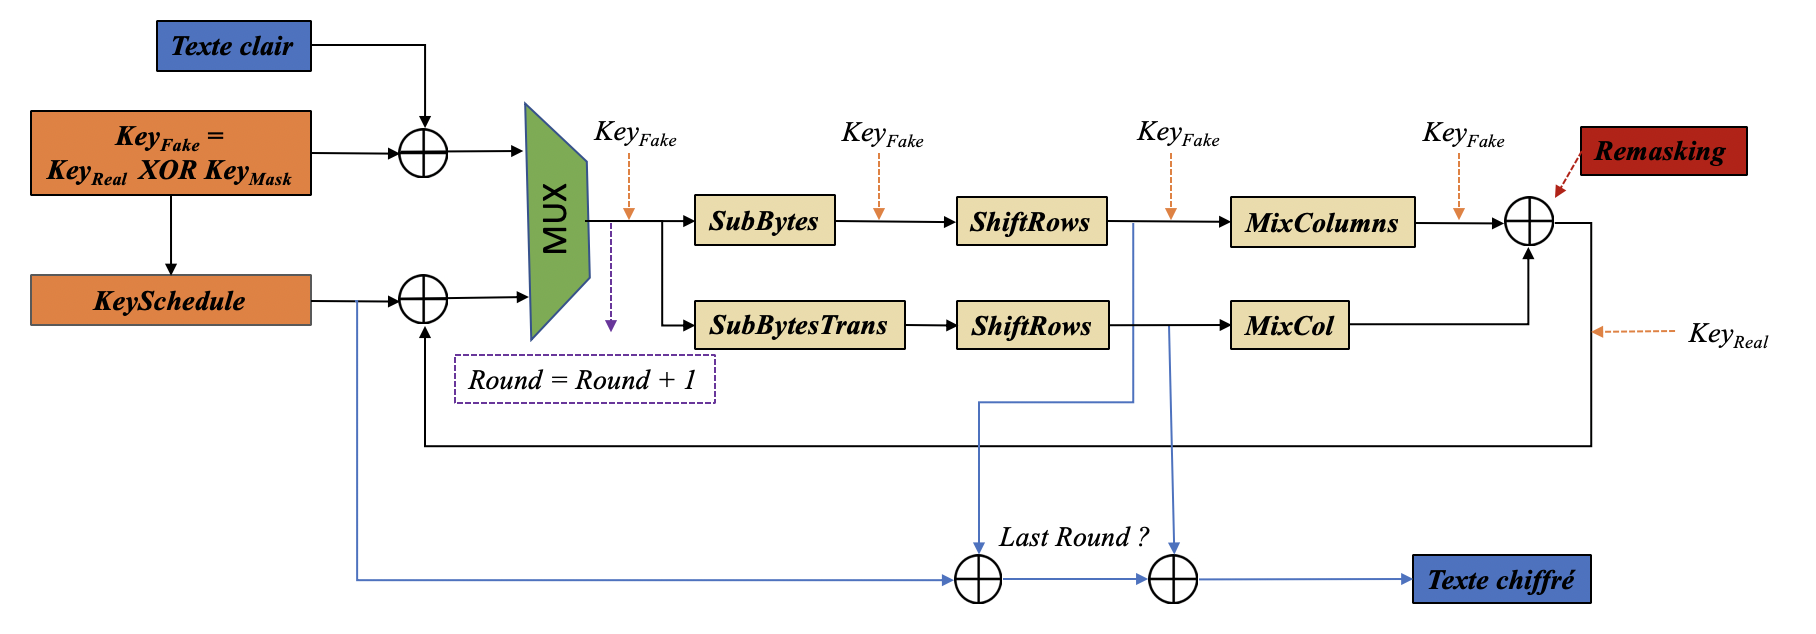
\includegraphics[scale=0.52]{image/ConceptFaking}
    \caption{Implémentation de la contre-mesure \textit{faking} pour l'algorithme de chiffrement AES.}
    \label{fig:ConceptFaking} 
\end{figure}

Dans les contre-mesures de type \textit{Masking}, lorsqu'on applique un masque sur les données intermédiaires, il faut ensuite le retirer de façon à obtenir \textit{in fine} le \textit{vrai} texte chiffré. Pour le cas des contre-mesures de type \textit{Faking}, le principe est identique. En effet, si aucune action supplémentaire n'est entreprise, le texte chiffré serait crypté avec la fausse clé plutôt qu'avec la vraie clé. Pour ce faire, on va ajouter deux nouvelles opérations dont le rôle est d'annuler l'emploi du masque sur la clé. Ces deux opérations sont \textit{SubBytesTrans} et \textit{MixCol}. Enfin, afin de définitivement couper tout lien des résultats intermédiaires avec la fausse clé, un XOR (opération \textit{remasking}) est opéré entre les résultats intermédiaires obtenus après \textit{MixColumns} et ceux obtenus après \textit{MixCol}. Le résultat de ce XOR permet de retirer l'emploi du masque, on retrouve alors le résultat que l'on aurait obtenu en sortie de l'opération \textit{MixColumns} si on avait utilisé la vraie clé initialement (voir équation \ref{eqn:faking_7}). Ceci est visible sur la figure \ref{fig:ConceptFaking}. Ensuite, l'opération \textit{AddRoundKey} emploie à nouveau une fausse clé, dérivant de l'opération \textit{KeySchedule}.

Définissons la nouvelle opération \textit{SubBytesTrans}. Pour ce faire, notons $Key_{Fake}(i,j)$ (avec $i \ \epsilon \ [0:3]$ et $j \ \epsilon \ [0:3]$) la fausse clé utilisée, $Key_{Real}(i,j)$ la vraie clé utilisée et $P(i,j)$ l'ensemble de textes clairs (\textit{plaintext} en anglais) envoyés au device crytpographique. Notons également $a_{F}(i,j)$ un byte particulier à la sortie de l'opération \textit{ShiftRows} chiffré avec la fausse clé $Key_{Fake}$ (voir figure \ref{fig:ConceptFaking}) et notons $a_{R}(i,j)$ un byte particulier à la sortie de l'opération \textit{ShiftRows} mais cette fois-ci chiffré avec la vraie clé $Key_{Real}$. Ces deux notations sont reprises à l'équation \ref{eqn:faking_2}.

\begin{gather}
	\left\{\begin{matrix}
	a_{F}(i,j) = ShiftRows(Key_{Fake}(i,j) \oplus P(i,j)) \\ 
	a_{R}(i,j) = ShiftRows(Key_{Real}(i,j) \oplus P(i,j))
	\end{matrix}\right.\label{eqn:faking_2}
\end{gather}

\hspace{-0.5cm}Étant donné que c'est la fausse clé qui est utilisée pour l'implémentation de la contre-mesure, si nous souhaitons obtenir le résultat intermédiaire à la sortie de l'opération \textit{SubBytes}, nous avons la relation \ref{eqn:faking_3} :
\begin{gather}
	Sbox(a_{F}(i,j)) = Sbox(ShiftRows(Key_{Fake}(i,j) \oplus P(i,j)))\label{eqn:faking_3}
\end{gather}

\hspace{-0.5cm}Connaissant la relation \ref{eqn:faking}, nous pouvons ré-écrire l'équation \ref{eqn:faking_3} sous la forme suivante : 
\begin{gather}
	Sbox(a_{F}(i,j)) = Sbox(ShiftRows(Key_{Real}(i,j) \oplus Key_{Mask}(i,j) \oplus P(i,j)))\label{eqn:faking_4}
\end{gather}

\hspace{-0.5cm}Ainsi, une façon simple de retrouver le byte original $a_{R}(i,j)$ utilisé avec la clé réelle à la sortie de l'opération \textit{SubBytes} est de définir une nouvelle fonction, appelée \textit{SubBytesTrans}. Cette fonction est donc définie sur base de l'équation \ref{eqn:faking_4} de la manière suivante : 
\begin{gather}
	Sbox(a_{F}(i,j)) = Sbox(ShiftRows(Key_{Real}(i,j) \oplus P(i,j))) \oplus SubBytesTrans(i,j)\label{eqn:faking_5}
\end{gather}

\hspace{-0.5cm}En effet, selon l'équation \ref{eqn:faking_2}, on peut simplifier l'équation précédente \ref{eqn:faking_5} par l'équation suivante \ref{eqn:faking_6} où l'on retrouve bien le byte original $a_{R}(i,j)$.
\begin{gather}
	Sbox(a_{F}(i,j)) = Sbox(a_{R}(i,j)) \oplus SubBytesTrans(a_{F}(i,j))\label{eqn:faking_6}
\end{gather}

\hspace{-0.5cm}Autrement dit, la fonction \textit{SubBytesTrans} se traduit par :
\begin{gather}
	SubBytesTrans(a_{F}(i,j)) = Sbox(a_{R}(i,j))  \oplus Sbox(a_{F}(i,j)) \label{eqn:faking_7}
\end{gather}

\hspace{-0.5cm}Concernant la nouvelle opération \textit{MixCol}, il ne s'agit en réalité pas d'une nouvelle opération étant donné que cette opérations réalise la même fonction que l'opération \textit{MixColumns} (tel que décrit à la section \ref{subsec:AES}). Cependant, nous précisons à la section suivante (\ref{subsec:points}) que \textit{MixCol} permet d'éviter une faille dans la contre-mesure. C'est donc la raison pour laquelle, le \textit{remarsking} (opération XOR) ne se fait pas avant cette opération.

\subsection{Points faibles et améliorations}
\label{subsec:points}

Deux points faibles de l'implémentation de la contre-mesure faking proposés à la figure \ref{fig:ConceptFaking} sont repris ci-dessous et améliorés afin de diminuer grandement les chances de réussite de l'attaquant.
\begin{enumerate}
\item Le but de la contre-mesure faking est d'autoriser l'attaquant à trouver une fausse valeur de clé. Cependant, connaissant la valeur de cette faussé clé, si l'attaquant trouve la valeur du masque, il peut retrouver la valeur de la vraie clé selon l'équation \ref{eqn:faking}. Ainsi, pour améliorer ce problème, il faut que chaque byte du masque utilisé ($Key_{mask}$) soit différent. Ceci complique la tâche de l'attaquant.
\item Il existe une attaque utilisant les résultats intermédiaires à la sortie des opérations \textit{SubBytes} et \textit{SubBytesTrans} et qui permet de retrouver la clé réelle. En effet, si l'attaquant récupère ces deux valeurs intermédiaires et qu'il réalise un XOR entre eux, il obtient la simplification suivante : 
\begin{gather}
\begin{align*}
        Sbox(a_{F}(i,j)) \oplus SubBytesTrans(a_{F}(i,j)) &= Sbox(a_{R}(i,j))  \\
            &=Sbox(ShiftRows(Key_{Real}(i,j) \oplus State(i,j)))  
\end{align*}
\label{eqn:faille1}
\end{gather}

En considérant le premier round de l'AES-256, l'élément $State(i,j)$ représente un texte clair ($P(i,j)$). Dans ce cas, connaissant le fonctionnement des opérations \textit{ShiftRows} et \textit{SubBytes}, l'attaquant peut retrouver la valeur de la vraie clé $Key_{Real}$. Pour se prémunir de ce problème, une amélioration de la contre-mesure faking consiste à masquer les valeurs en sortie de l'opération \textit{SubBytesTrans}. En effet, à chaque round, un masque aléatoire $M_{h}(i,j)$ est appliqué sur les résultats intermédiaires en sortie de l'opération \textit{SubBytesTrans} de sorte à obtenir l'équation suivante \ref{eqn:faille1_solution} : 
\begin{gather}
	SubBytesTrans(a_{F}(i,j)) = Sbox(a_{R}(i,j))  \oplus Sbox(a_{F}(i,j)) \oplus M_{h}(i,j) \label{eqn:faille1_solution}
\end{gather}
Notons que le masque $M_{h}(i,j)$ est renouvelé de façon aléatoire à chaque round pour complexifier le chiffrement. Ce masque $M_{h}(i,j)$ devient le masque $M_{k}(i,j)$ après l'exécution de l'opération \textit{MixColumns}. 
\end{enumerate}

\newpage

\hspace{-0.5cm}La figure \ref{fig:ConceptFakingWithMasking} présente le principe de fonctionnement de la contre-mesure faking avec les améliorations apportées.
\begin{figure}[htbp]
    \hspace{-1.2cm}
    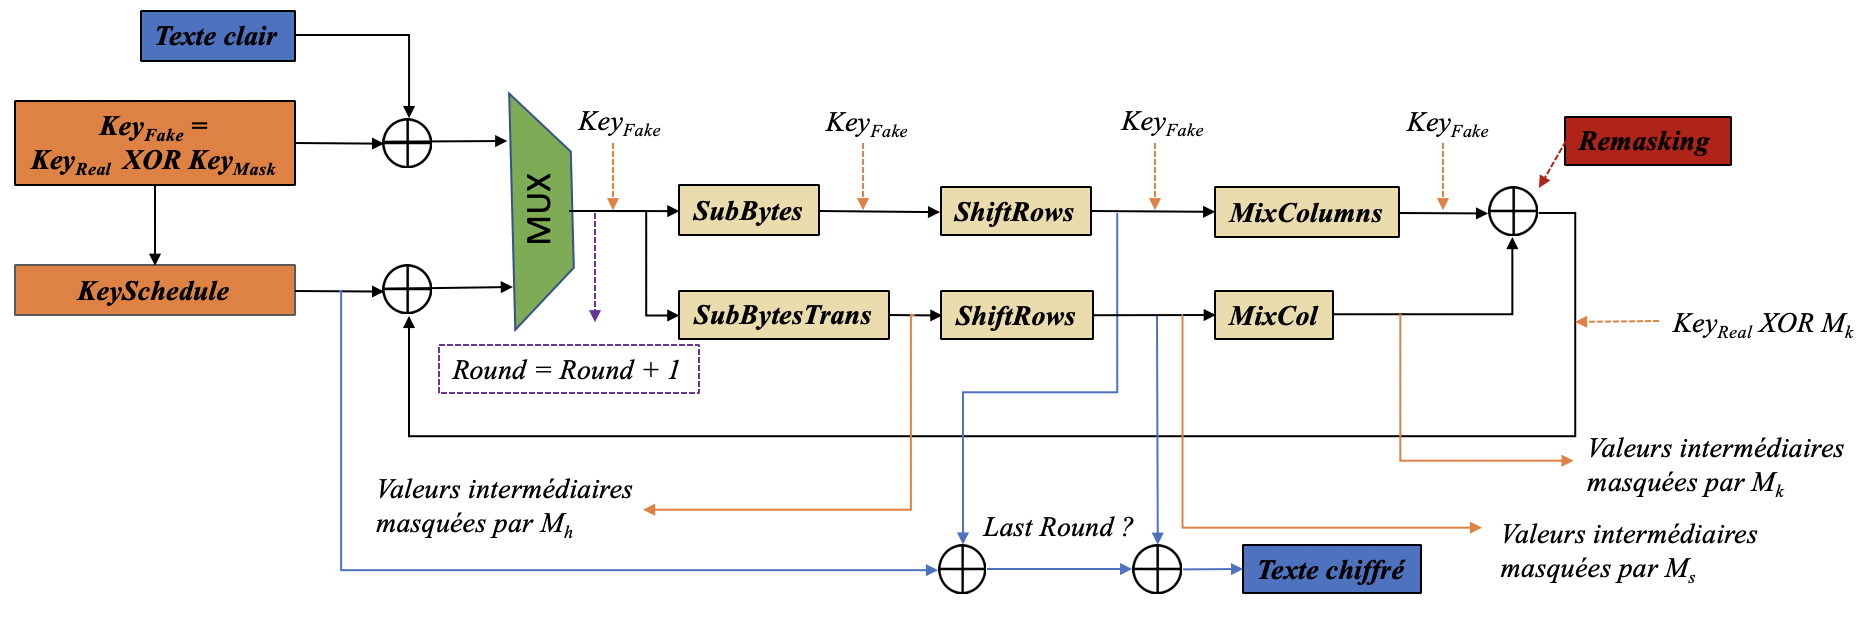
\includegraphics[scale=0.58]{image/ConceptFakingWithMasking}
    \caption{Implémentation de la contre-mesure \textit{faking} pour l'algorithme de chiffrement AES avec prise en compte des améliorations.}
    \label{fig:ConceptFakingWithMasking} 
\end{figure}


Reprenons l'exemple du chapitre précédent (chapitre \ref{chap:attaques}) où l'on présentait les résultats (voir figures \ref{fig:4KeysEx} et \ref{fig:TrueKey}) d'une attaque CPA sur un FPGA implémentant l'algorithme AES-256. Pour rappel, l'attaque est réalisée sur le huitième byte de la clé dont la valeur attendue est 40. Considérons maintenant avoir implémenté une contre-mesure de type faking sur le device cryptographique (il s'agit d'une simulation réalisée sur MATLAB). Dans ce cas, si l'attaquant réalise une nouvelle attaque CPA sur le device, la clé qu'il obtient doit être différente de la vraie clé utilisée. Ceci se vérifie sur la figure \ref{fig:fakingExemple}. La vraie clé utilisée pour le chiffrement des données (40) ne laisse fuiter aucune information. Par contre, la clé laissant fuiter le plus d'information est bien la fausse clé (185). En effet, la valeur du masque étant 145, selon l'équation \ref{eqn:faking}, nous trouvons :
\begin{gather}
\hspace{-5cm}\begin{align*}
        Key_{Fake} &= Key_{Real} \oplus Key_{Mask}  \\
            &= 40 \oplus 145 \\
            &= 185  
\end{align*}
\end{gather}

\begin{figure}[htbp]
    \vspace{-0.6cm}
    \centering
    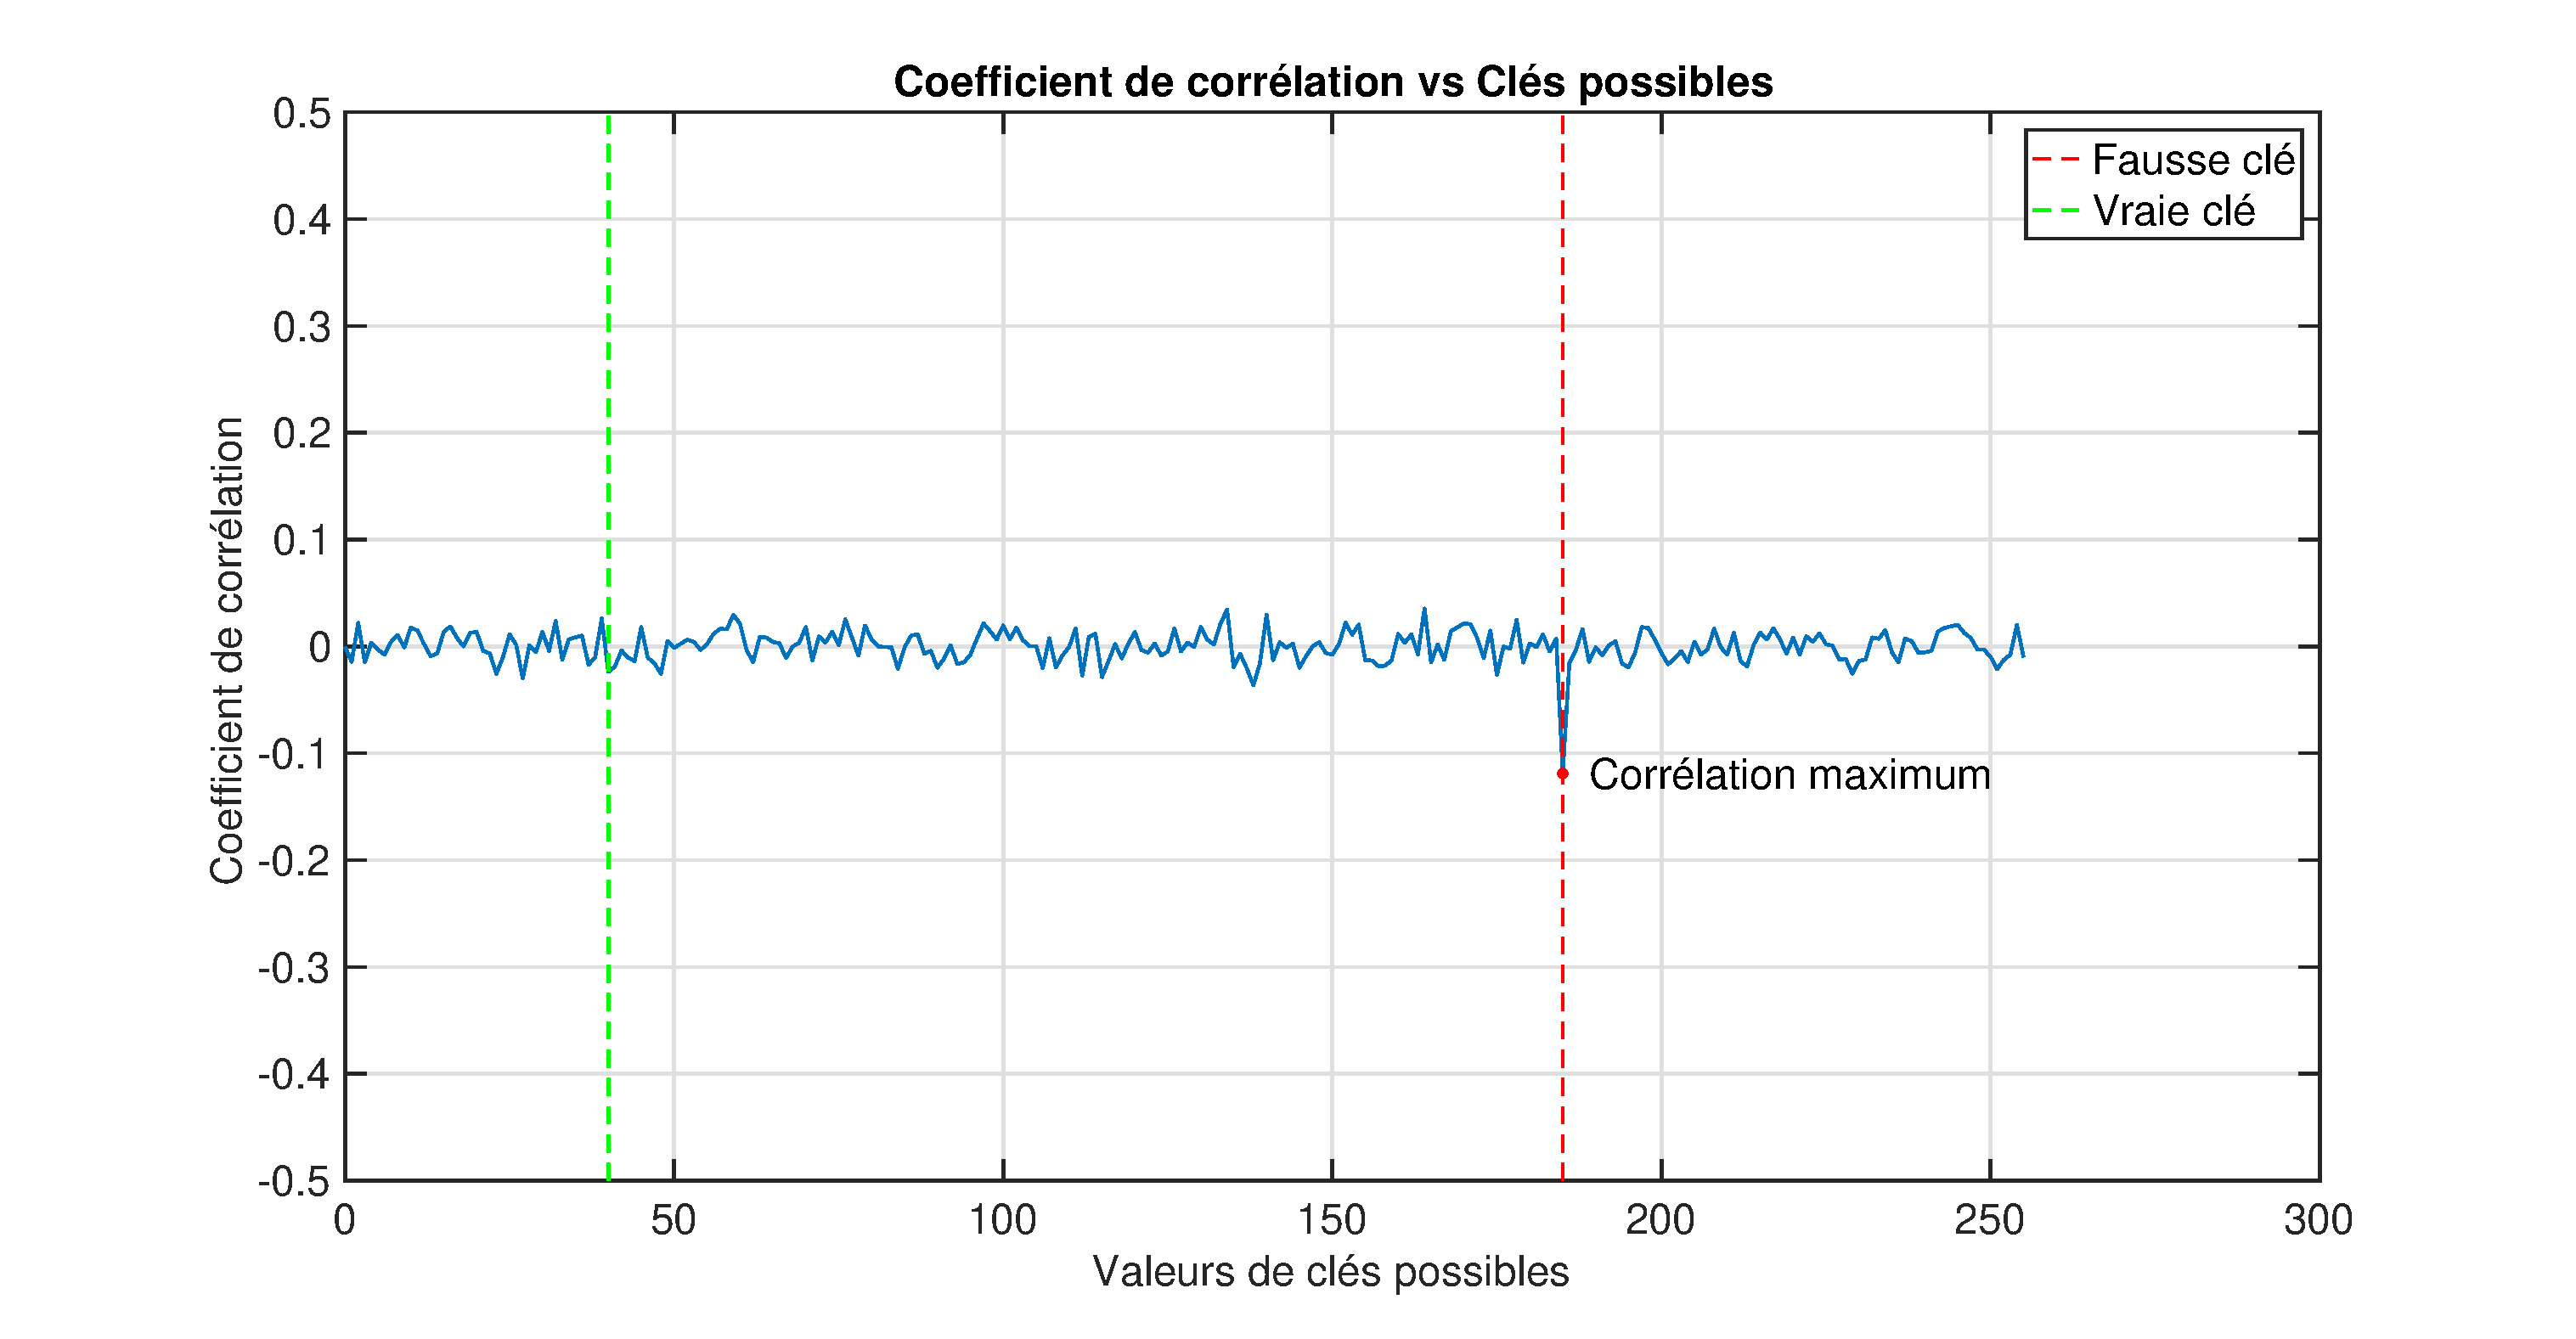
\includegraphics[scale=0.30]{image/fakingExemple}
    \caption{Valeur de la clé obtenue avec implémentation d'une contre-mesure faking.}
    \label{fig:fakingExemple} 
\end{figure}


\newpage


%%%%%%%%%%%%%%%%%%%%%%%%%%%%%%%%%%%%%%%%%%%%%%%%%%%%%%%%%%%%%%
%                                                                            Partie 2 - Pratique                     								 %
%%%%%%%%%%%%%%%%%%%%%%%%%%%%%%%%%%%%%%%%%%%%%%%%%%%%%%%%%%%%%%

\part{Mise en application}

%%%%%%%%%%%%% Chapitre 6 %%%%%%%%%%%%%

\chapter{Mise en oeuvre de l'attaque}
\label{chap:config}

Ce chapitre décrit la mise en oeuvre de l'attaque CPA. Une introduction sur les différents langages utilisées est tout apportée. Ensuite, trois sections sont respectivement réservées à la description de la configuration du FPGA, à la description de la configuration de l'oscilloscope et enfin à la description de la configuration de l'attaque.

\section{Langages de programmation}
\label{sec:langages}

\hspace{-0.5cm}Trois langages de programmation ont été utiles à la réalisation de ce travail : 
\begin{itemize}
\item \textbf{\textit{PYTHON}} pour la configuration de la communication entre l'ordinateur et le FPGA et entre l'ordinateur et l'oscilloscope ;
\item \textbf{\textit{VHDL}} (\textit{VHSIC Hardware Description Language}) pour l'implémentation de l'algorithme AES-256 et de la contre-mesure \textit{Faking} sur le FPGA ;
\item \textbf{\textit{MATLAB}} (\textit{MATrix LABoratory}) pour d'une part la mise en application de l'attaque CPA et d'autre part les simulations et réalisations de graphes utiles à la compréhension des notions théoriques. \\
\end{itemize}


\section{Procédure de chiffrement et configuration de l'oscilloscope}
\label{sec:config_chiff}

\hspace{-0.5cm}La liste du matériel nécessaire pour le chiffrement de messages clairs est présentée ci-dessous : 

\hspace{-0.5cm}\textbf{Un device cryptographique} : le device cryptographique employé pour implémenter l'algorithme AES-256 est un FPGA. Plus précisément, il s'agit d'une carte de test spécialement conçue pour de la recherche et développement dans le domaine de la sécurité matérielle. Cette carte, visible sur la figure \ref{fig:sakura} et portant le nom \textit{SAKURA-G}, est en effet utilisée pour réaliser des attaques par canaux cachés mais également d'autres types d'attaques physiques comme les attaques par injections de fautes, etc. Cette carte intègre deux FPGAs de la famille \textit{Spartan-6} : l'un est utilisé comme contrôleur (\textit{Controller FPGA}) et l'autre comme circuit principal de sécurité (\textit{Main FPGA}). Pour la réalisation de ce travail, le FPGA principal est configuré pour chiffrer des données (il implémente l'algorithme AES-256) tandis que le contrôleur est utilisé pour gérer la communication entre le FPGA principal et l'ordinateur. La fréquence d'horloge pour ces deux FPGA est de 48 MHz. Il est à noter qu'il existe trois points de mesures sur la carte SAKURA-G pour analyser la consommation de puissance du FPGA principal. Ces trois connecteurs SMA (\textit{SubMiniature version A}) sont visibles sur la figure \ref{fig:sakura} et plus précisément sur la figure \ref{fig:mesurePoints}. À l'inverse des connecteurs $J_1$ et $J_2$, le connecteur $J_3$ amplifie la consommation de puissance du FPGA principal (section \ref{sec:CPA}). Enfin, cette carte peut être alimentée de deux façons différentes : soit par le port USB soit par une alimentation externe.

\newpage

\begin{figure}[htbp]
    \centering
    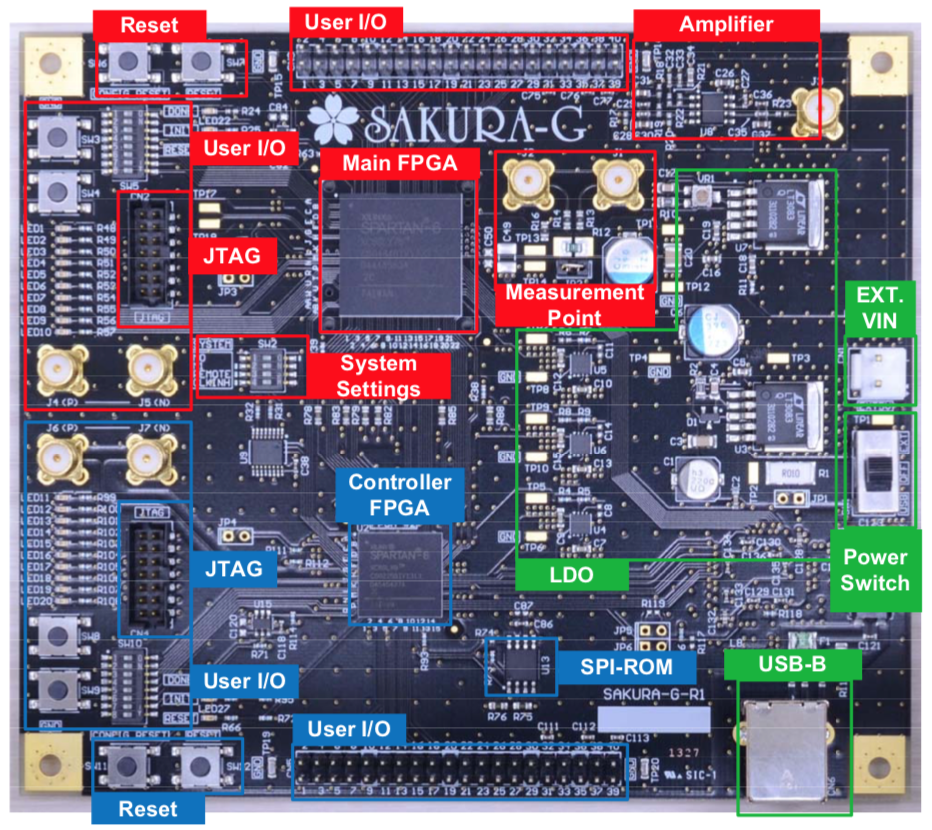
\includegraphics[scale=0.69]{image/Sakura}
    \caption{Carte SAKURA-G.}
    \label{fig:sakura} 
\end{figure}

\begin{figure}[htbp]
    \centering
    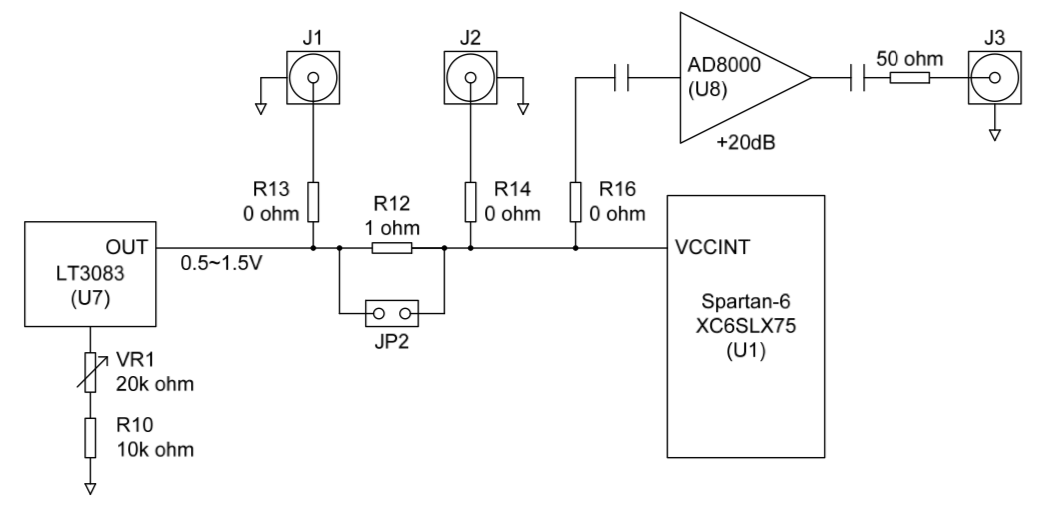
\includegraphics[scale=0.62]{image/points_mesures}
    \caption{Les trois points de mesures utilisés pour déterminer la consommation de puissance (la tension pour être exact) du FPGA principal.}
    \label{fig:mesurePoints} 
\end{figure}

\hspace{-0.5cm}\textbf{Alimentation de laboratoire} : Comme précisé ci-avant, il existe deux moyen d'alimenter la carte SAKURA-G : soit par l'interface du port USB, soit par une alimentation externe. Par expérience d'un ancien étudiant, il s'avère que l'alimentation via le port USB est instable, ce qui rend l'analyse de la consommation de puissance plus compliquée. Pour cette raison, une alimentation de laboratoire est utilisée et alimente la carte en $5V\pm 5\%$ (avec courant limité à 3A).  

\hspace{-0.5cm}\textbf{Oscilloscope} : L'oscilloscope est l'instrument de mesure utilisé pour capturer la consommation de puissance du device cryptographique (FPGA) lorsque celui-ci est en cours de chiffrement. L'oscilloscope utilisé est un Picoscope de la série 5000D possédant deux canaux de mesures (A et B) (voir figure \ref{fig:picoscope}). Ce Picoscope possède une bande passante de 200 MHz et un échantillonnage pouvant aller jusqu'à 1 Gé/s. Sa résolution peut être configurée sur 8, 12, 14, 15 ou 16 bits. La particularité de cet oscilloscope est que l'affichage, les commandes et l'alimentation (USB) s'effectuent exclusivement à partir de l'ordinateur auquel il est branché. Il existe une interface logicielle (voir figure \ref{fig:picoscope_interface}) permettant de le configurer. Cependant pour la réalisation de ce travail, l'oscilloscope sera configuré et utilisé via un script python (utilisant une librairie en référence à ce Picoscope). Le tableau \ref{tab:picoscope} présente les paramètres de configuration du Picoscope utilisés dans ce travail pour la prise des mesures sur le FPGA.

\begin{figure}[htbp]
    \centering
    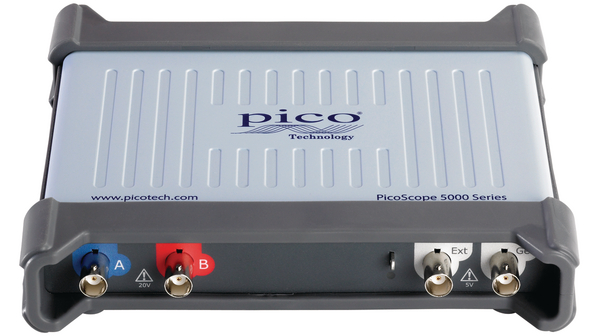
\includegraphics[scale=0.38]{image/picoscope}
    \caption{Le Picoscope est l'instrument de mesure utilisé pour analyser la consommation de puissance (tension) du FPGA.}
    \label{fig:picoscope} 
\end{figure}

\begin{figure}[htbp]
    \centering
    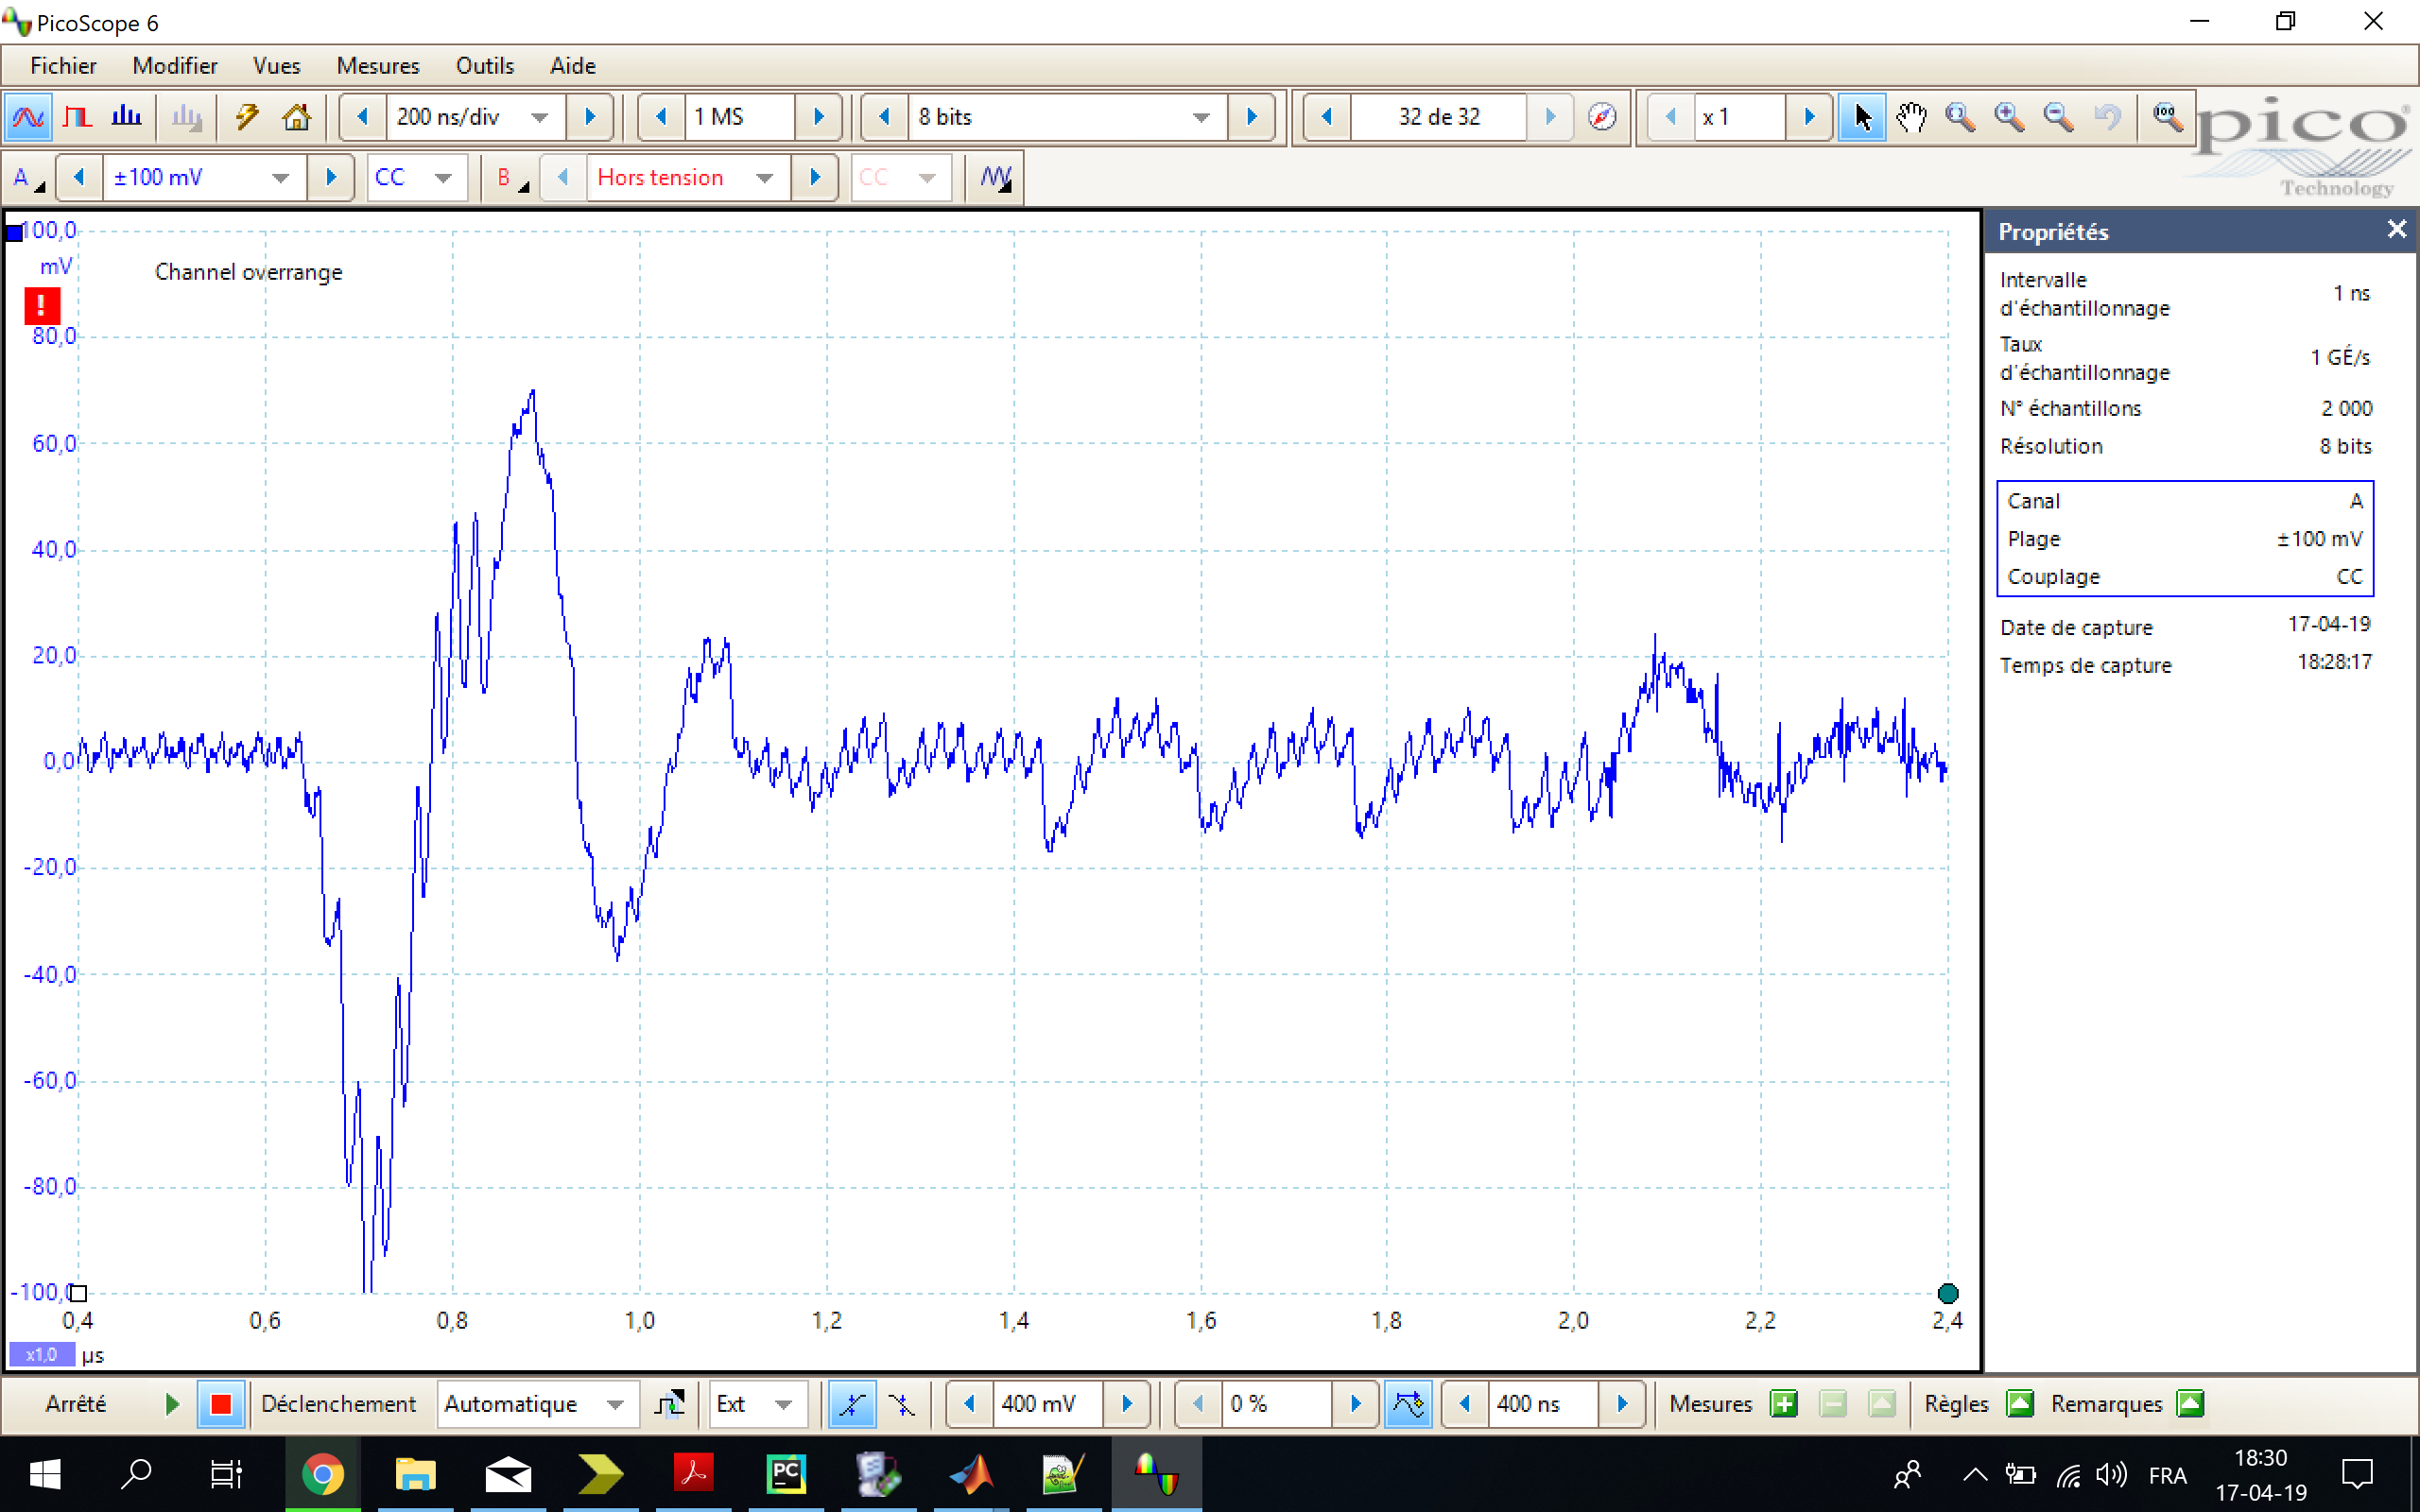
\includegraphics[scale=0.45]{image/picoscope_interface}
    \caption{Interface logicielle du Picoscope présentant une trace de puissance du FPGA en cours de chiffrement.}
    \label{fig:picoscope_interface} 
\end{figure}

\begin{table}[htbp]
	\hspace{-1.2cm}
	\begin{tabular}{|c||c|c|c|c|}
    		\hline
  		  \textbf{Canal} &\textbf{ Couplage} & \textbf{Plage de tension ($mv$)} & \textbf{Résolution} & \textbf{Nombre d'échantillons} \\ \hline 
		  Canal A & AC & \pm200 & 12 bits & 755\\ \hline 
  		  Canal B &  / & / & / & / \\ \hline \hline 
 		  \textbf{Canal} &  \textbf{Seuil de déclenchement ($mv$)} & \textbf{Sur flanc} & \textbf{délai ($ms$)} & \textbf{Post trigger ($ns$)} \\ \hline
 		  Canal Ext &  40 & montant & 3000 & 1510 \\ \hline
	\end{tabular}
    	\caption{Paramètres des canaux A, B et Ext du Picoscope.}
    	\label{tab:picoscope} 
\end{table}


\newpage

\hspace{-0.5cm}\textbf{Ordinateur} : 


\newpage

\hspace{-0.5cm}La figure \ref{fig:procedure_1} décrit la procédure générale utilisée pour configurer les différents systèmes informatiques employés (FPGA, oscilloscope, ordinateur) ainsi que pour chiffrer différents messages clairs. Cette procédure se compose de six étapes décrites ci-après. Pour cette procédure, on considère que le code VHDL de l'algorithme AES-256 est déjà implémenté sur le FPGA. 
\begin{enumerate}
\item Configuration du protocole de communication entre l'oscilloscope et l'ordinateur (Python)  ;
\item Configuration du protocole de communication entre le FPGA et l'ordinateur (Python) ;
\item Envoi de la clé de chiffrement ($K$) et d'un texte clair ($P$) au FPGA depuis l'ordinateur (Python)  ;
\item Chiffrement du message clair sur le FPGA et génération d'un trigger par la FPGA pour aligner les traces sur l'oscilloscope (VHDL) ;
\item Une fois le chiffrement du message clair terminé :
\begin{enumerate}
\item Sauvegarde sur ordinateur de la trace de puissances capturée à l'oscilloscope (Python) ;
\item Sauvegarde sur ordinateur du message chiffré par le FPGA (Python) ;
\end{enumerate}
\item Étant donné qu'il faut envoyer un grand nombre (N) de messages clairs au FPGA pour que l'attaque CPA fonctionne (voir section \ref{sec:CPA}) : répétition des étapes 3 à 5 jusqu'à ce le nombre de messages clairs à envoyés soit atteint.
\end{enumerate}

\begin{figure}[htbp]
    \centering
    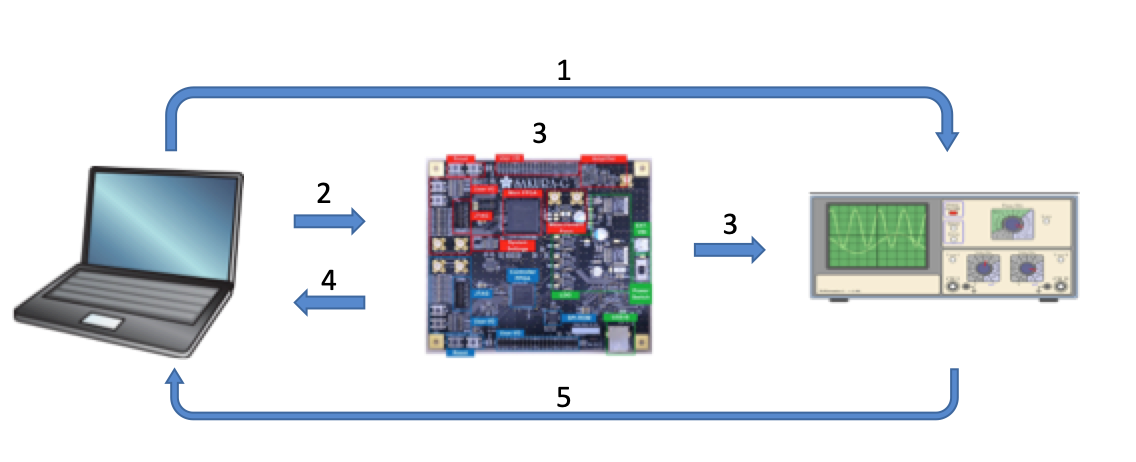
\includegraphics[scale=0.6]{image/procedure_1}
    \caption{Procédure mise en place pour le chiffrement de textes clairs et l'enregistrement des traces de puissance capturées à l'oscilloscope.}
    \label{fig:procedure_1} 
\end{figure}


\newpage

\section{Configuration de l'attaque CPA}
\label{sec:CPA_App}

\hspace{-0.5cm}La figure \ref{} ci-dessous décrit la procédure générale utilisée pour appliquer une attaque CPA sur l'implémentation de l'algorithme AES-256 sur un FPGA. Cette procédure se compose de six étapes décrites ci-après. Pour cette procédure, on considère que l'enregistrement des traces (procédure précédente) a déjà été réalisé. De plus, cette procédure est entièrement réalisée avec le logiciel MATLAB.
\begin{enumerate}
\item Récupération et chargement des traces de puissance capturées à l'oscilloscope ;
\item Récupération et chargement des $N$ messages clairs envoyés au FPGA pour être chiffrés ;
\item Simulation des opérations \textit{AddRoundKey} et \textit{SubBytes} permettant de tester toutes les valeurs de clés possibles ;
\item Prédiction de la puissance consommée par utilisation d'un modèle de puissance (Poids de Hamming) ;
\item Calcul de la corrélation entre les traces de puissance et les prédictions de consommation ;
\item Détermination de la clé secrète sur base de la corrélation maximum ;
\end{enumerate}

\newpage

%%%%%%%%%%%%% Chapitre 7 %%%%%%%%%%%%%

\chapter{Mise en application d'une attaque CPA (\textit{Correlation Power Analysis})}

\section{Résultats de simulations}
\label{sec:Introduction}

\section{Résultats expérimentaux}
\label{sec:Introduction}

\section{Conclusion}
\label{sec:Introduction}

\newpage

%%%%%%%%%%%%% Chapitre 8 %%%%%%%%%%%%%

\chapter{Implémentation de la contre-mesure de type \textit{faking}}
\label{chap:faking}

\section{Développement de la contre-mesure}
\label{sec:Introduction}

\subsection{Résultats expérimentaux}
\label{sec:Introduction}

\section{Conclusion}
\label{sec:Introduction}

\newpage

%%%%%%%%%%%%% Chapitre 9 %%%%%%%%%%%%%

\chapter{Évaluation des performances de la contre-mesure}

\section{Évaluation par métriques}
\label{sec:EvalMetrics}

\section{Évaluation par critères de performances}
\label{sec:EvalPerf}

\newpage

%%%%%%%%%%%%% Chapitre 10 %%%%%%%%%%%%%

\chapter{Conclusion}

Ancienne conclusion ... (stage)

Nous vivons dans une société de consommation où les technologies évoluent sans cesse. Il y a 40 ans, la gestion des signaux relevait de la science-fiction. Il y a 25 ans, les GSM constituaient une innovation majeure. Aujourd’hui, tout le monde se demande comment il était possible de vivre à cette époque sans toutes ces nouvelles technologies ! Le sujet qu'il m'a été proposé d'étudier durant ces 6 semaines de stage en immersion fut, à première vue, aussi complexe qu'inconnu. En effet, ce sujet, les attaques par canaux cachés, est encore assez méconnu à ce jour dans le domaine de l'ingénierie. Tenter d'expliquer à quiconque qu'il est possible de subtiliser des données sensibles précautionneusement chiffrées par divers algorithmes, à partir de moyens simples (oscilloscope, ordinateurs, ...) et de calculs élémentaires, semble au premier abord, difficilement concevable. 

Depuis ces découvertes à la fin des années 90, la sécurité matérielle a pris une tournure particulière pour les grandes industries telles que Thales. C'est désormais sur un nouvel axe de recherche, s'écartant des sentiers traditionnels, que se porte la problématique de protection de données sensibles. Imaginez qu'un algorithme utilisé pour chiffrer des données bancaires puisse être cassé par simple application d'une attaque par canaux cachés ? Il n'est donc pas anormal de voir certaines industries développer leurs propres contre-mesures pour s'affranchir contre ce type d'attaque. Certes, avant de développer des contre-mesures, il est nécessaire, dans un premier temps, de bien comprendre les fondements des attaques par canaux cachés. Certes, la compréhension des notions théoriques et leurs mises en pratique est une tâche ardue qui nécessite la compréhension et l'intégration de concepts très spécifiques. Néanmoins, je suis convaincu que ce type d'attaque va, au fils des années, devenir une piste d'enseignement sérieuse et nécessaire aux futurs ingénieurs en électronique.

À titre personnel, je tire un bilan très positif de ce stage d'immersion. Il fut très enrichissant. Ces 6 semaines de stage sont passées à la vitesse de l'éclair : plongeant à certains moments dans les articles scientifiques et livres de références rédigés sur le sujet ; à d'autres dans les simulations MATLAB afin de mieux assimiler les concepts ; ou encore à discuter avec les étudiants stagiaires afin de partager notre expérience de stage. 6 semaines, c'est assez court mais déjà suffisant pour une première introduction sur les attaques par canaux cachés et les contre-mesures qu'il est possible d'implémenter. L'ensemble des objectifs fixés avant le début de stage (énoncés à la section \ref{sec:objectifs}) a pu être traité et atteint. Étant désormais convaincu de la puissance de ce type d'attaque, développer des contre-mesures me paraît constituer un challenge intéressant et très utile dans le cadre de la protection des données sensibles. Je vais donc désormais pouvoir m'attaquer à la phase suivante, consécutive à ce stage, mon Travail de Fin d'Étude. Ce TFE consistera à développer une contre-mesure contre les attaques par canaux cachés.




\newpage
%%%%%%%%%%%%%%%%%%%%%%%% CREDITS %%%%%%%%%%%%%%%%%%%%
\phantomsection
\section*{Crédits}
\addcontentsline{toc}{section}{Crédits}

\begin{itemize}

\item Figure~\ref{fig:thales} provenant du site internet :
\url{http://monipag.com/victoria-petitier/wp-content/uploads/sites/1363/Thales-Group-1.png}

\item Figure~\ref{fig:CMOS} provenant du site internet :
\url{https://hal.archives-ouvertes.fr/hal-00753215/document}

\item Annexe~\ref{ann:Sbox} provenant du site internet de J.M. Dutertre \textit{"Synthèse AES 128"} :
\url{https://www.emse.fr/~dutertre/documents/synth_AES128.pdf}

\item Annexe~\ref{ann:ConceptFaking} provenant du site internet UPCommons \textit{"Faking Countermeasure Against Side-Channel Attacks"} :
\url{https://upcommons.upc.edu/bitstream/handle/2117/112973/Advances_in_Microelectronics_V_1_chapter19.pdf?sequence=1}

\end{itemize}

%%%%%%%%%%%%%%%%%%%%%%%% REFERENCES %%%%%%%%%%%%%%%%%%%%

\phantomsection
\addcontentsline{toc}{section}{Références}

\nocite{*}
\bibliography{Stage}
\bibliographystyle{unsrt}


%%%%%%%%%%%%%%%%%%%%%%%% ANNEXES %%%%%%%%%%%%%%%%%%%%
\newpage
\lhead{}
\addcontentsline{toc}{chapter}{Annexes}
\DeactivateToc

\begin{appendices}
%%%%% Annexe chapitre 2
\phantomsection
\chapter{Liste des annexes du chapitre \ref{chap:crypto}}

\begin{itemize}
\item Annexe \ref{ann:CESAR} : Chiffre de César.
\item Annexe \ref{ann:AES128} : Code algorithme AES-128 - Ordre d'exécution des opérations.
\item Annexe \ref{ann:AES256} : Code algorithme AES-256 - Ordre d'exécution des opérations.
\item Annexe \ref{ann:Sbox} : Sbox - Table de substitution.
\item Annexe \ref{ann:KeySchedule} : Opération \textit{KeySchedule}.
\end{itemize}

\newpage

\rhead{ANNEXE \ref{ann:CESAR}}
\section{Chiffre de César}
\label{ann:CESAR}
\vspace{2cm}

\begin{table}[htbp]
	\centering
	\begin{tabular}{|c|c|}
    		\hline
   		  \textbf{Texte clair} & \textbf{Texte chiffré}  \\ \hline 
		  A & D \\ \hline
		  B & E \\ \hline	
		  C & F \\ \hline
		  D & G \\ \hline	
		  E & H \\ \hline
		  F & I \\ \hline	
		  G & J \\ \hline
		  H & K \\ \hline	
		  I & L \\ \hline
		  J & M \\ \hline	
		  K & N \\ \hline
		  L & O \\ \hline	
		  M & P \\ \hline
		  N & Q \\ \hline	
		  O & R \\ \hline
		  P & S \\ \hline	
		  Q & T \\ \hline
		  R & U \\ \hline	
		  S & V \\ \hline
		  T & W \\ \hline	
		  U & X \\ \hline
		  V & Y \\ \hline	
		  W & Z \\ \hline
		  X & A \\ \hline	
		  Y & B \\ \hline
		  Z & C \\ \hline	
	\end{tabular}
 	\caption{Chiffre de César.}
 	\label{tab:CESAR}
\end{table}

\hspace{-0.5cm}Exemple : le message clair \textit{"chiffrement"} devient le message chiffré \textit{"fkliiuhphqw"}. En effet, le détail du procédé de chiffrement est donné à la table \ref{tab:CesarEx}.

\begin{table}[htbp]
	\centering
	\begin{tabular}{|c|c|c|c|c|c|c|c|c|c|c|c|}
    		\hline
   		  Message clair & C & H & I & F & F & R & E & M & E & N & T \\ \hline 
   		  Message chiffré & F & K & L & I & I & U & H & P & H & Q & W  \\ \hline 
	\end{tabular}
 	\caption{Exemple de chiffre de César.}
 	\label{tab:CesarEx}
\end{table}

\newpage


\rhead{ANNEXE \ref{ann:AES128}}
\phantomsection
\section{Code algorithme AES-128 - Ordre d'exécution des opérations.}
\label{ann:AES128}
\lstset{language=Pascal}          % Set your language (you can change the language for each code-block optionally)
\begin{lstlisting}[frame=single]  % Start your code-block

Require : STATE, Key
Ensure : STATE

KeySchedule(Key)
AddRoundKey(STATE, ExpandedKey[0])
for i=1 < 10 do
	SubBytes(STATE)
	ShiftRows(STATE)
	MixColumns(STATE)
	AddRoundKey(STATE, ExpandedKey[i])
	i = i + 1
end for
SubBytes(STATE)
ShiftRows(STATE)
AddRoundKey(STATE, ExpandedKey[10])
\end{lstlisting}

\newpage

\rhead{ANNEXE \ref{ann:AES256}}
\phantomsection
\section{Code algorithme AES-256 - Ordre d'exécution des opérations.}
\label{ann:AES256}
\lstset{language=Pascal}          % Set your language (you can change the language for each code-block optionally)
\begin{lstlisting}[frame=single]  % Start your code-block

Require : STATE, Key
Ensure : STATE

KeySchedule(Key)
AddRoundKey(STATE, ExpandedKey[0])
for i=1 < 14 do
	SubBytes(STATE)
	ShiftRows(STATE)
	MixColumns(STATE)
	AddRoundKey(STATE, ExpandedKey[i])
	i = i + 1
end for
SubBytes(STATE)
ShiftRows(STATE)
AddRoundKey(STATE, ExpandedKey[10])
\end{lstlisting}

\newpage

\rhead{ANNEXE \ref{ann:Sbox}}

\section{Sbox - Table de substitution}
\label{ann:Sbox}
\begin{table}[htbp]
	\centering
	\begin{tabular}{|c||c|c|c|c|c|c|c|c|c|c|c|c|c|c|c|c|}
		  \hline
		  & 0 & 1 & 2 & 3 & 4 & 5 & 6 & 7 & 8 & 9 & a & b & c & d & e & f \\ \hline \hline
		  0 & 63 & 7c & 77 & 7b & f2 & 6b & 6f & c5 & 30 & 01 & 67 & 2b & fe & d7 & ab & 76   \\ \hline	
		  1 & ca & 82 & c9 & 7d & fa & 59 & 47 & f0 & ad & d4 & a2 & af & 9c & a4 & 72 & c0   \\ \hline	
		  2 & b7 & fd & 93 & 26 & 36 & 3f & f7 & cc & 34 & a5 & e5 & f1 & 71 & d8 & 31 & 15   \\ \hline	
		  3 & 04 & c7 & 23 & c3 & 18 & 96 & 05 & 9a & 07 & 12 & 80 & e2 & eb & 27 & b2 & 75   \\ \hline	
		  4 & 09 & 83 & 2c & 1a & 1b & 6e & 5a & a0 & 52 & 3b & d6 & b3 & 29 & e3 & 2f & 84   \\ \hline	
		  5 & 53 & dl & 00 & ed & 20 & fc & b1 & 5b & 6a & cb & be & 39 & 4a & 4c & 58 & cf   \\ \hline	
		  6 & d0 & ef & aa & fb & 43 & 4d & 33 & 85 & 45 & f9 & 02 & 7f & 50 & 3c & 9f & a8   \\ \hline	
		  7 & 51 & a3 & 40 & 8f & 92 & 9d & 38 & f5 & bc & b6 & da & 21 & 10 & ff & f3 & d2   \\ \hline	
		  8 & cd & 0c & 13 & ec & 5f & 97 & 44 & 17 & c4 & a7 & 7e & 3d & 64 & 5d & 19 & 73   \\ \hline	
		  9 & 60 & 81 & 4f & dc & 22 & 2a & 90 & 88 & 46 & ee & b8 & 14 & de & 5e & 0b & db   \\ \hline	
		  a & e0 & 32 & 3a & 0a & 49 & 06 & 24 & 5c & c2 & d3 & ac & 62 & 91 & 95 & e4 & 79   \\ \hline	
		  b & e7 & c8 & 37 & 6d & 8d & d5 & 4e & a9 & 6c & 56 & f4 & ea & 65 & 7a & ae & 08   \\ \hline	
		  c & ba & 78 & 25 & 2e & 1c & a6 & b4 & c6 & e8 & dd & 74 & 1f & 4b & bd & 8b & 8a   \\ \hline	
		  d & 70 & 3e & b5 & 66 & 48 & 03 & f6 & 0e & 61 & 35 & 57 & b9 & 86 & c1 & 1d & 9e   \\ \hline	
		  e & e1 & f8 & 98 & 11 & 69 & d9 & 8e & 94 & 9b & 1e & 87 & e9 & ce & 55 & 28 & df   \\ \hline	
		  f & 8c & a1 & 89 & 0d & bf & e6 & 42 & 68 & 41 & 99 & 2d & 0f & b0 & 54 & bb & 16   \\ \hline	
	\end{tabular}
 	\caption{La Sbox représente une table de substitution utilisée pour l'opération non-linéaire SubBytes de l'algorithme AES. À chaque donnée hexadécimale d'entrée correspond une donnée hexadécimale de sortie.}
 	\label{fig:Sbox}
\end{table}

\newpage

\rhead{ANNEXE \ref{ann:KeySchedule}}
\section{Opération \textit{KeySchedule}}
\label{ann:KeySchedule}
\begin{figure}[htbp]
    \centering
    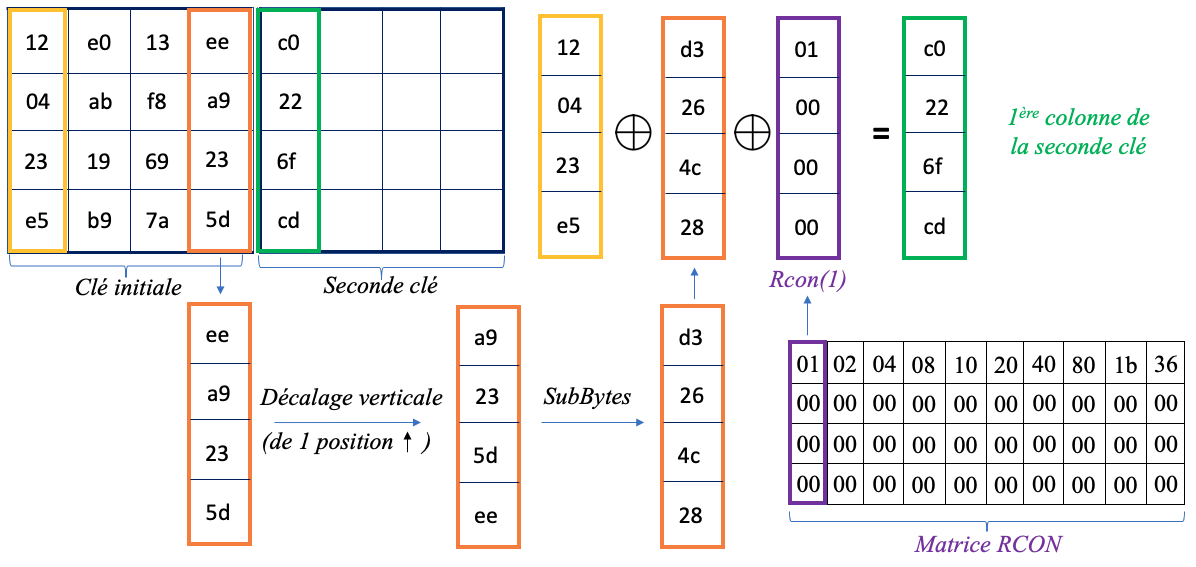
\includegraphics[scale=0.35]{image/KeySchedule1}
    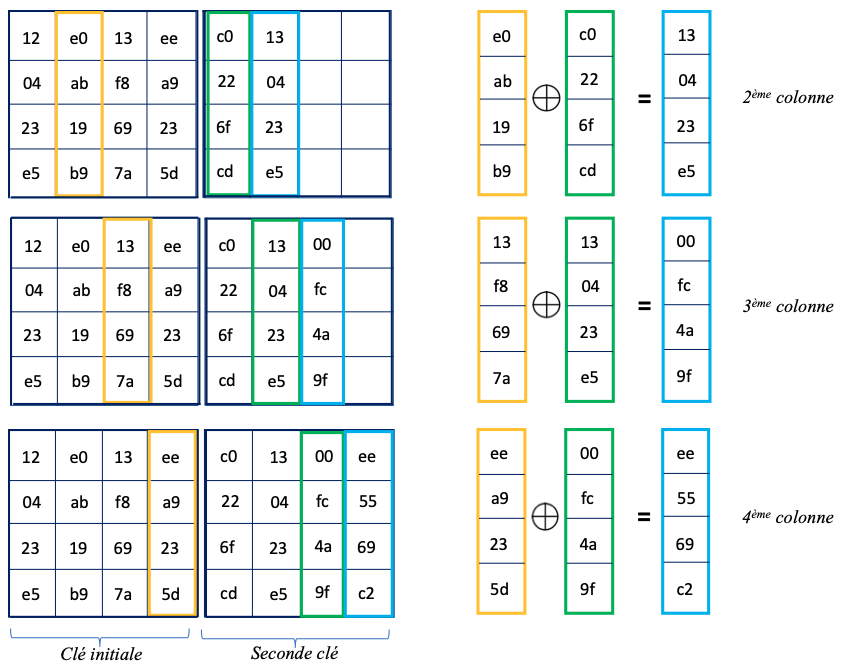
\includegraphics[scale=0.45]{image/KeySchedule2}
    \caption{Principe de fonctionnement de l'opération \textit{KeySchedule}.}
    \label{fig:KeySchedule1}
\end{figure}

\newpage

%%%%% Annexe chapitre 3

%%%%% Annexe chapitre 4
\chapter{Liste des annexes du chapitre \ref{chap:attaques}}
\begin{itemize}
\item Annexe \ref{ann:traceExplain} : Représentation des traces de puissance prises à l'oscilloscope.
\end{itemize}

\newpage

\rhead{ANNEXE \ref{ann:traceExplain}}
\section{Représentation des traces de puissance prises à l'oscilloscope.}
\label{ann:traceExplain}
\begin{figure}[htbp]
    \centering
    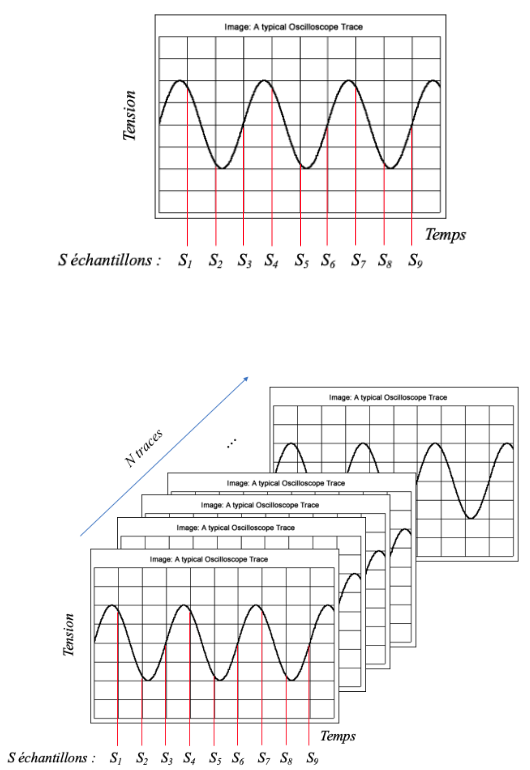
\includegraphics[scale=0.65]{image/Sampling}
    \caption{La figure du haut représente une trace de puissance (i.e 1 plaintext utilisé) dans laquelle on retrouve 9 échantillons. La figure du bas représente N traces de puissance dans lesquelles on retrouve également 9 échantillons. En pratique, le nombre d'échantillons dans une trace de puissance est beaucoup plus élevé (de l'ordre de 10000) et sera noté par la lettre S (pour \textit{Sampling}).}
    \label{fig:traceExplain}
\end{figure}

\newpage

%%%%% Annexe chapitre 5
\chapter{Liste des annexes du chapitre \ref{chap:contremesure}}
\begin{itemize}
\item Annexe \ref{ann:resume_hiding} : Contre-mesures \textit{Hiding}.
\end{itemize}

\newpage

\rhead{ANNEXE \ref{ann:resume_hiding}}
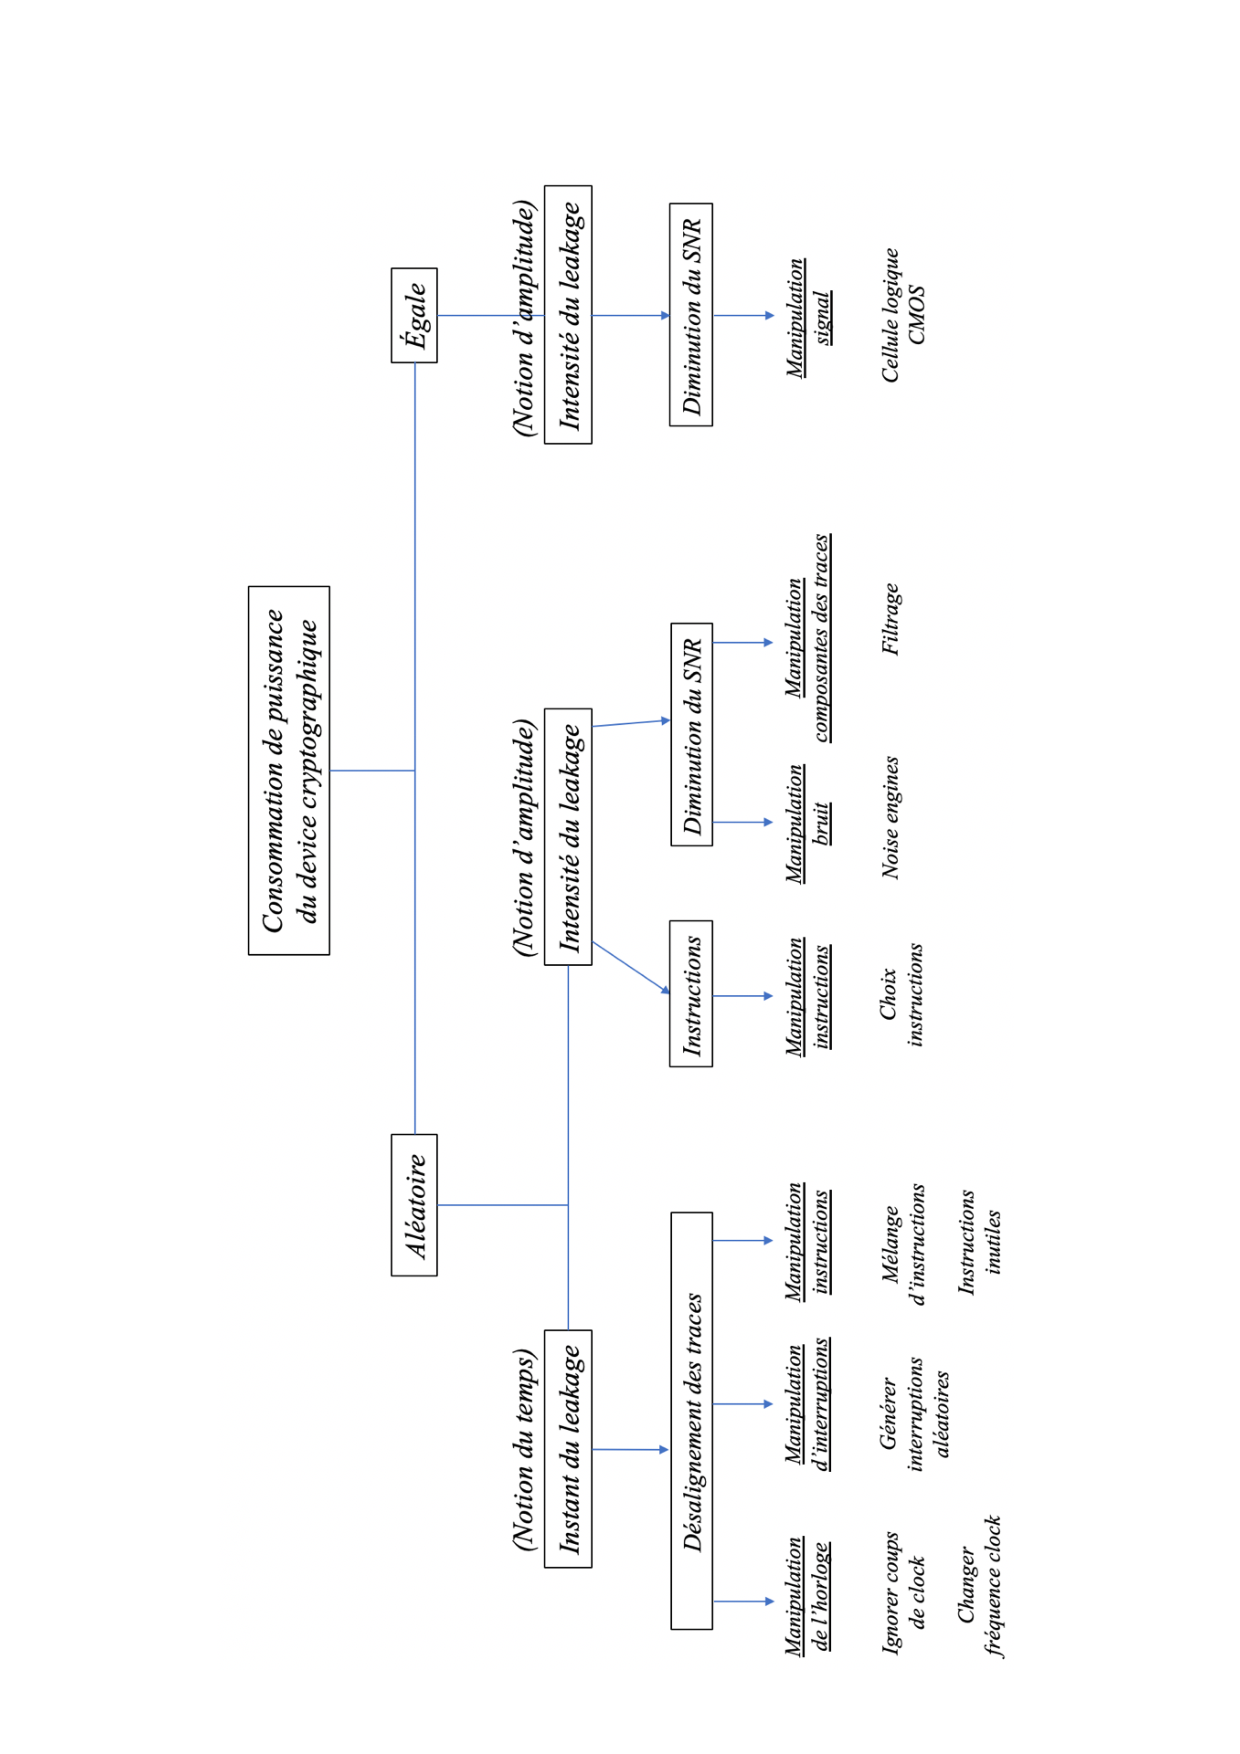
\includepdf[pagecommand=\section{Contre-mesures \textit{Hiding}}\label{ann:resume_hiding}]{image/resume_hiding.pdf}

%\rhead{ANNEXE \ref{ann:resume_hiding}}
%\section{Contre-mesures \textit{Hiding}}
%\label{ann:resume_hiding}
%\begin{figure}[htb]
%    \centering
%    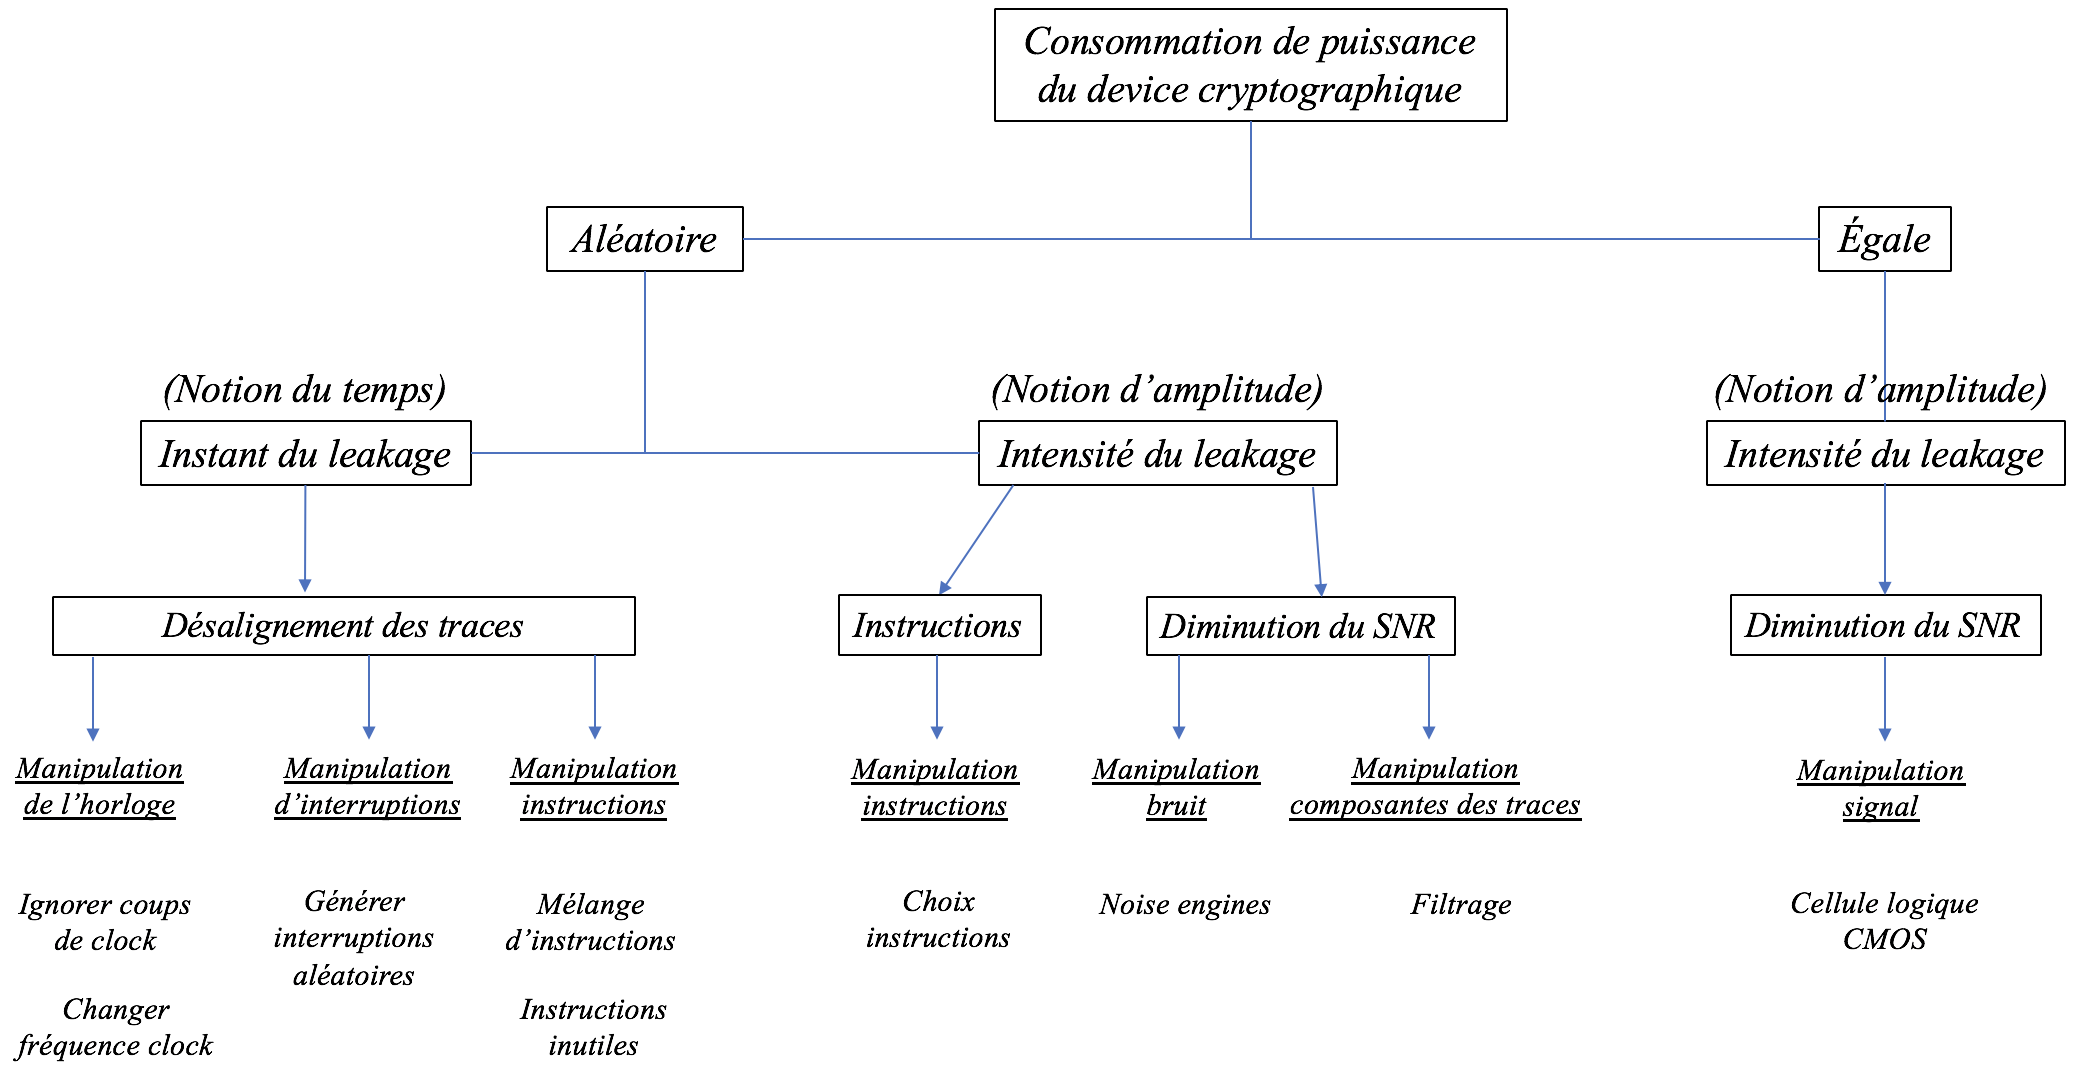
\includegraphics[width=1\linewidth, angle=90]{image/resume_hiding}
%    \caption{Ce schéma présente les différentes sortes de contre-mesures de type hiding.}
%    \label{fig:resume_hiding} 
%\end{figure}

\newpage

%%%%% Annexe autres
\chapter{Autres annexes}
\begin{itemize}
\item Annexe \ref{ann:lettre} : Lettre de motivation.
\item Annexe \ref{ann:certificat} : Certificat de stage.
\end{itemize}

\rhead{ANNEXE \ref{ann:lettre}}
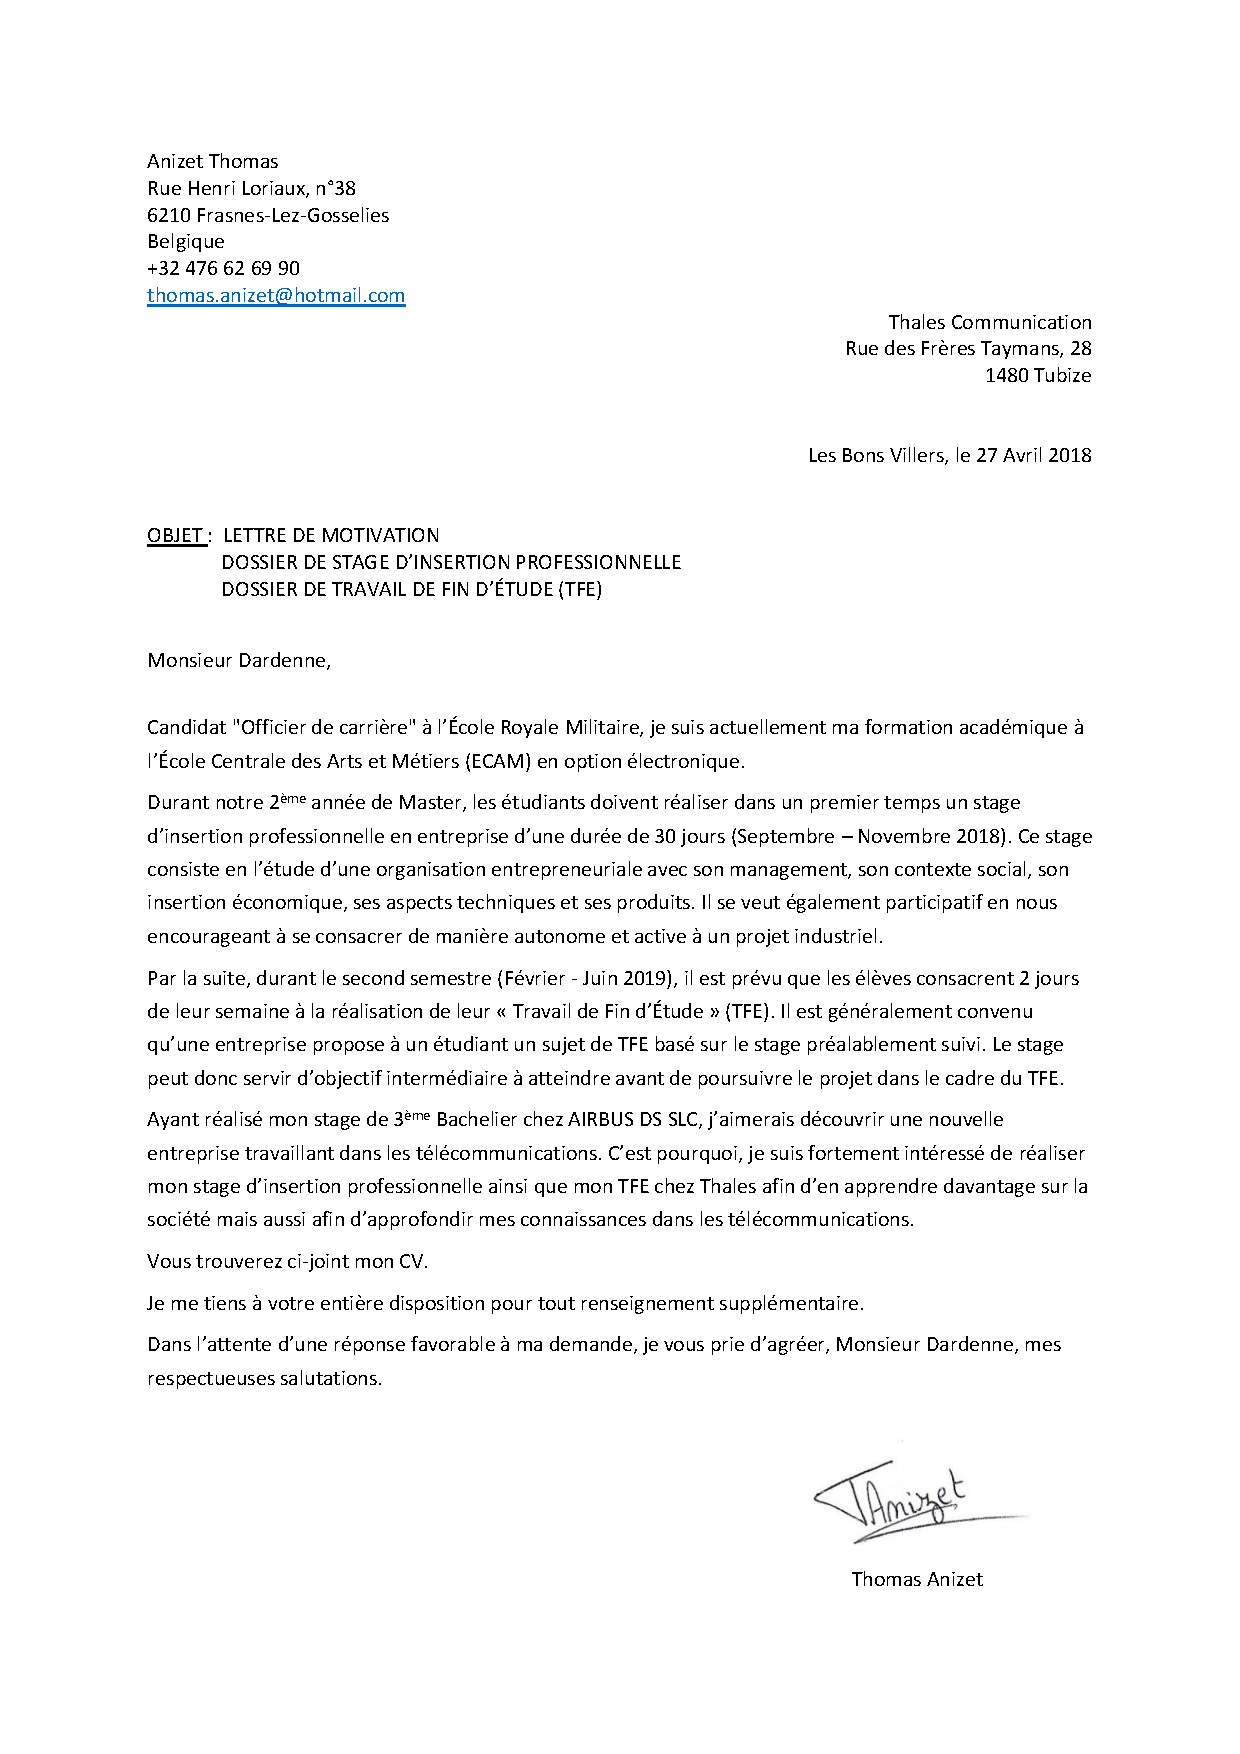
\includepdf[pagecommand=\section{Lettre de motivation}\label{ann:lettre}]{image/lettre.pdf}

\newpage

\rhead{ANNEXE \ref{ann:certificat}}
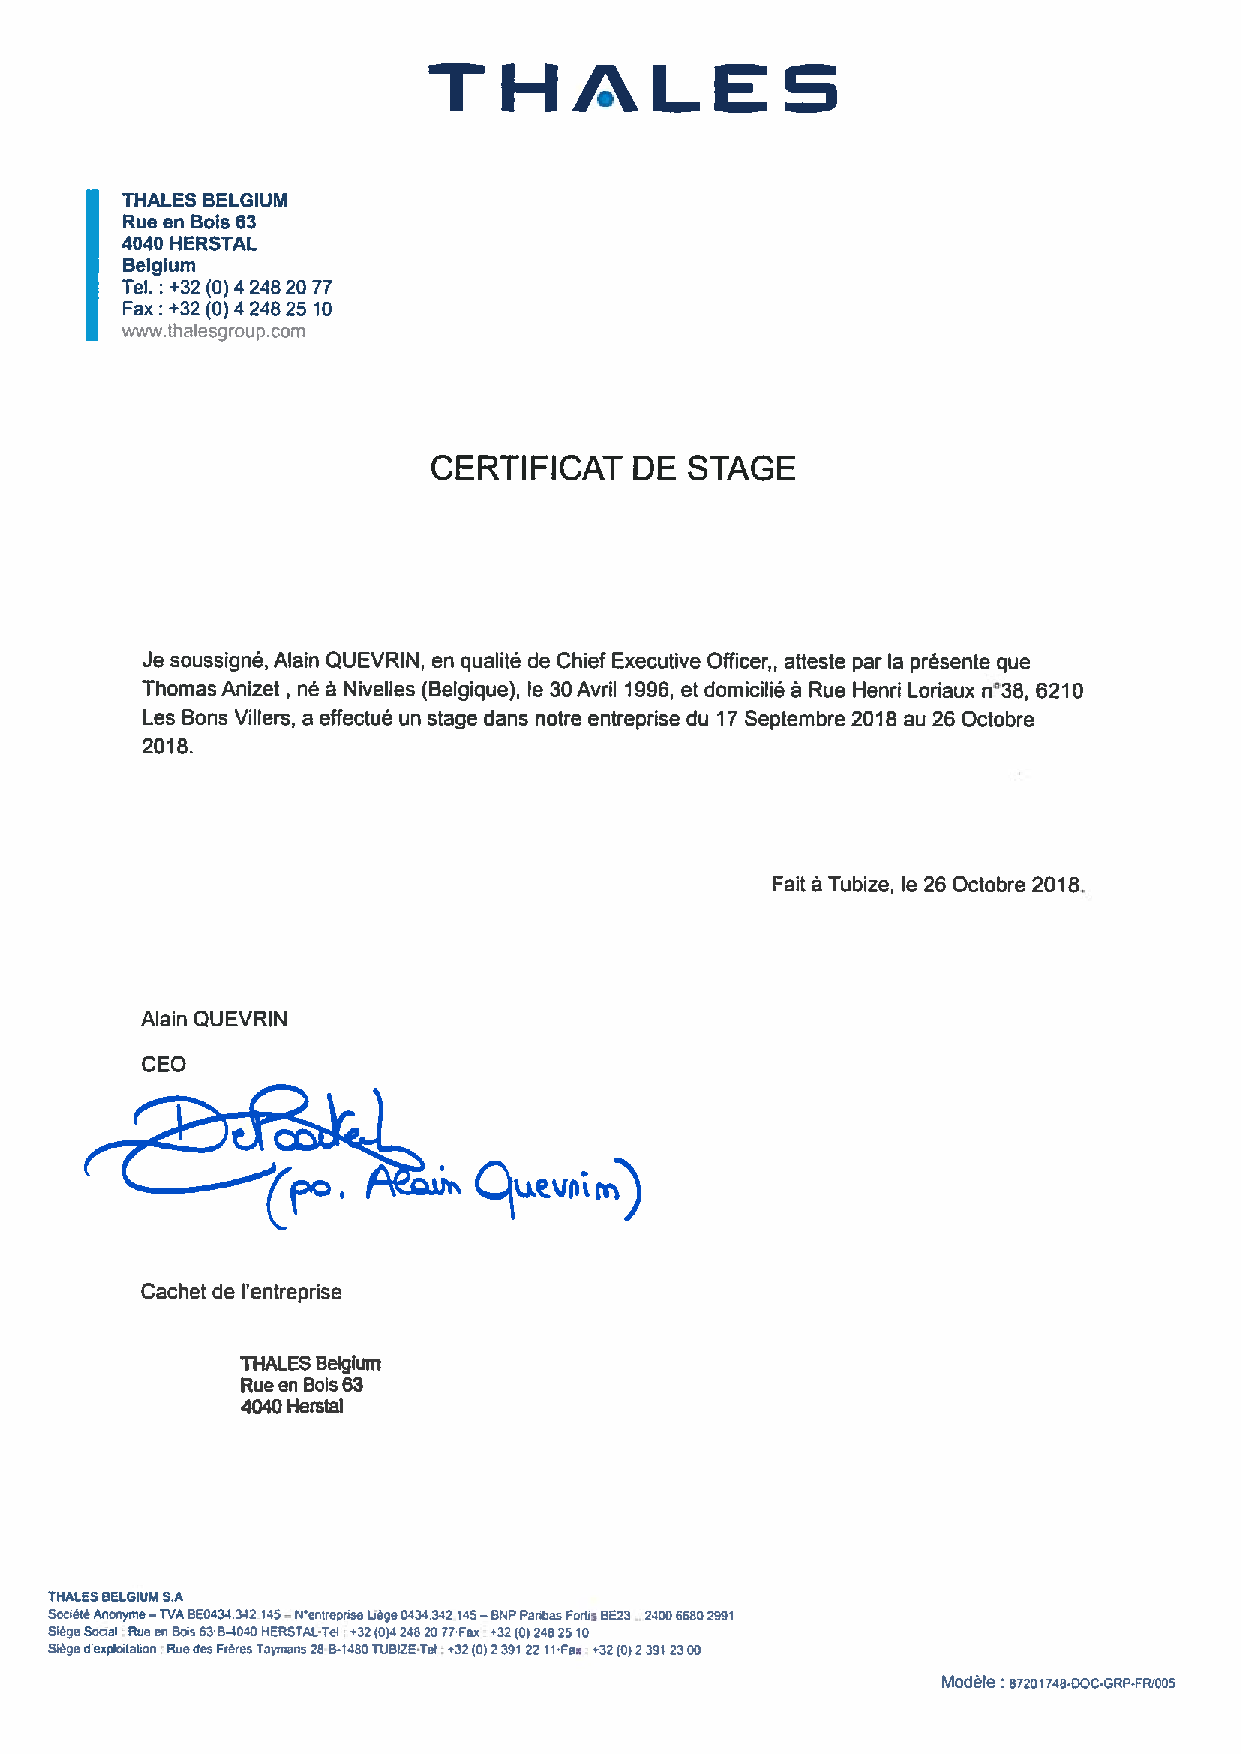
\includepdf[pagecommand=\section{Certificat de stage}\label{ann:certificat}]{image/certificat.pdf}


\end{appendices}

\end{document}
